%
% Copyright (c) 2006 XenSource, Inc.
%
% Permission is granted to copy, distribute and/or modify this document under
% the terms of the GNU Free Documentation License, Version 1.2 or any later
% version published by the Free Software Foundation; with no Invariant
% Sections, no Front-Cover Texts and no Back-Cover Texts.  A copy of the
% license is included in the section entitled
% "GNU Free Documentation License" or the file fdl.tex.
%
% Authors: Ewan Mellor, Richard Sharp, Dave Scott, Jon Harrop.
%

\chapter{API Reference}
\label{api-reference}


\section{Classes}
The following classes are defined:

\begin{center}\begin{tabular}{|lp{10cm}|}
\hline
Name & Description \\
\hline
{\tt session} & A session \\
{\tt task} & A long-running asynchronous task \\
{\tt VM} & A virtual machine (or 'guest') \\
{\tt host} & A physical host \\
{\tt host\_cpu} & A physical CPU \\
{\tt network} & A virtual network \\
{\tt VIF} & A virtual network interface \\
{\tt PIF} & A physical network interface (note separate VLANs are represented as several PIFs) \\
{\tt SR} & A storage repository \\
{\tt VDI} & A virtual disk image \\
{\tt VBD} & A virtual block device \\
{\tt VTPM} & A virtual TPM device \\
{\tt console} & A console \\
{\tt user} & A user of the system \\
{\tt debug} & A basic class for testing \\
\hline
\end{tabular}\end{center}
\section{Relationships Between Classes}
Fields that are bound together are shown in the following table: 
\begin{center}\begin{tabular}{|ll|l|}
\hline
{\em object.field} & {\em object.field} & {\em relationship} \\

\hline
VDI.VBDs & VBD.VDI & many-to-one\\
VDI.parent & VDI.children & one-to-many\\
VBD.VM & VM.VBDs & one-to-many\\
VIF.VM & VM.VIFs & one-to-many\\
VIF.network & network.VIFs & one-to-many\\
PIF.host & host.PIFs & one-to-many\\
PIF.network & network.PIFs & one-to-many\\
SR.VDIs & VDI.SR & many-to-one\\
VTPM.VM & VM.VTPMs & one-to-many\\
console.VM & VM.consoles & one-to-many\\
host.resident\_VMs & VM.resident\_on & many-to-one\\
host.host\_CPUs & host\_cpu.host & many-to-one\\
\hline
\end{tabular}\end{center}

The following represents bound fields (as specified above) diagramatically, using crows-foot notation to specify one-to-one, one-to-many or many-to-many
                   relationships:

\begin{center}\resizebox{0.8\textwidth}{!}{
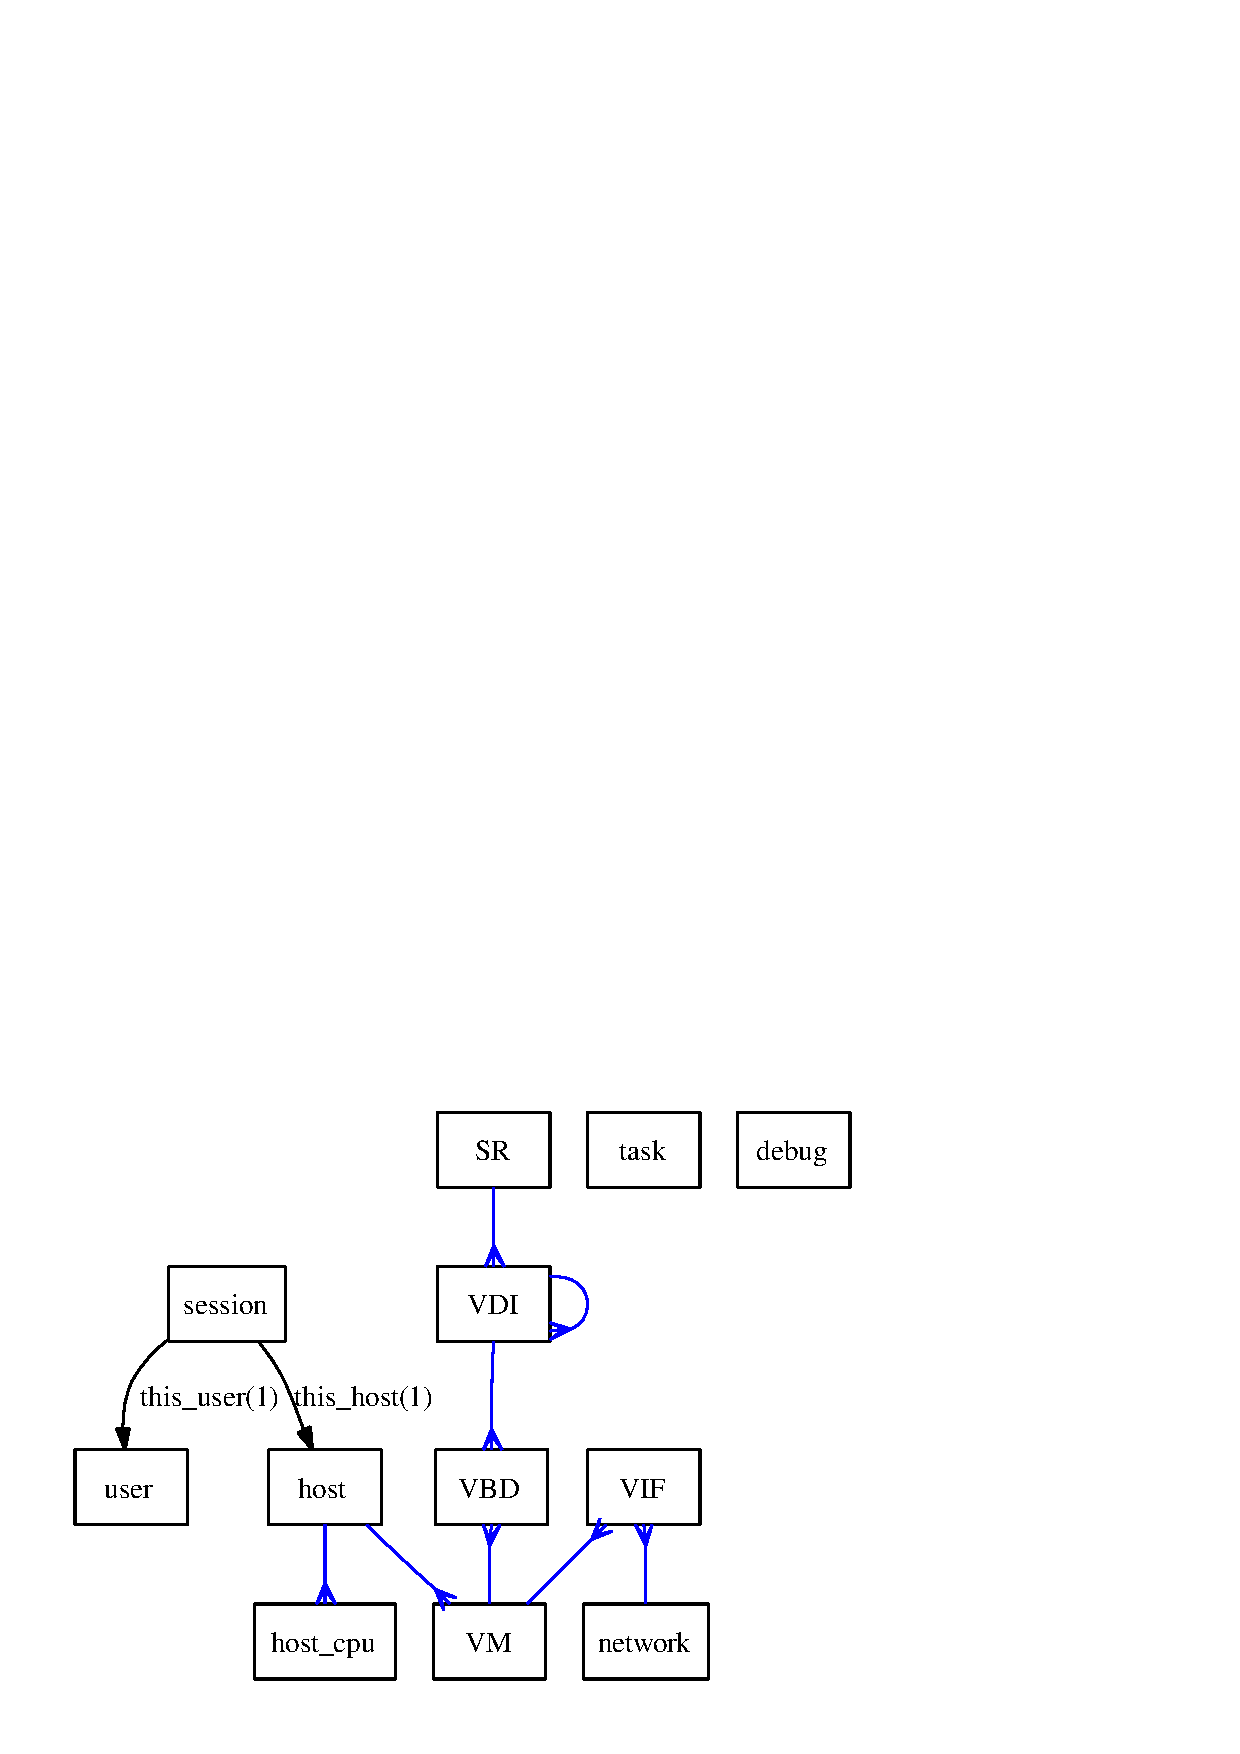
\includegraphics{xenapi-datamodel-graph}
}\end{center}
\
\subsection{List of bound fields}
\section{Types}
\subsection{Primitives}
The following primitive types are used to specify methods and fields in the API Reference:

\begin{center}\begin{tabular}{|ll|}
\hline
Type & Description \\
\hline
String & text strings \\
Int    & 64-bit integers \\
Float & IEEE double-precision floating-point numbers \\
Bool   & boolean \\
DateTime & date and timestamp \\
Ref (object name) & reference to an object of class name \\
\hline
\end{tabular}\end{center}
\subsection{Higher order types}
The following type constructors are used:

\begin{center}\begin{tabular}{|ll|}
\hline
Type & Description \\
\hline
List (t) & an arbitrary-length list of elements of type t \\
Map (a $\rightarrow$ b) & a table mapping values of type a to values of type b \\
\hline
\end{tabular}\end{center}
\subsection{Enumeration types}
The following enumeration types are used:

\begin{longtable}{|ll|}
\hline
{\tt enum console\_protocol} & \\
\hline
\hspace{0.5cm}{\tt vt100} & VT100 terminal \\
\hspace{0.5cm}{\tt rfb} & Remote FrameBuffer protocol (as used in VNC) \\
\hspace{0.5cm}{\tt rdp} & Remote Desktop Protocol \\
\hline
\end{longtable}

\vspace{1cm}
\begin{longtable}{|ll|}
\hline
{\tt enum vdi\_type} & \\
\hline
\hspace{0.5cm}{\tt system} & a disk that may be replaced on upgrade \\
\hspace{0.5cm}{\tt user} & a disk that is always preserved on upgrade \\
\hspace{0.5cm}{\tt ephemeral} & a disk that may be reformatted on upgrade \\
\hline
\end{longtable}

\vspace{1cm}
\begin{longtable}{|ll|}
\hline
{\tt enum vm\_power\_state} & \\
\hline
\hspace{0.5cm}{\tt Halted} & Halted \\
\hspace{0.5cm}{\tt Paused} & Paused \\
\hspace{0.5cm}{\tt Running} & Running \\
\hspace{0.5cm}{\tt Suspended} & Suspended \\
\hspace{0.5cm}{\tt ShuttingDown} & Shutting Down \\
\hspace{0.5cm}{\tt Unknown} & Some other unknown state \\
\hline
\end{longtable}

\vspace{1cm}
\begin{longtable}{|ll|}
\hline
{\tt enum task\_status\_type} & \\
\hline
\hspace{0.5cm}{\tt pending} & task is in progress \\
\hspace{0.5cm}{\tt success} & task was completed successfully \\
\hspace{0.5cm}{\tt failure} & task has failed \\
\hline
\end{longtable}

\vspace{1cm}
\begin{longtable}{|ll|}
\hline
{\tt enum cpu\_feature} & \\
\hline
\hspace{0.5cm}{\tt FPU} &  Onboard FPU  \\
\hspace{0.5cm}{\tt VME} &  Virtual Mode Extensions  \\
\hspace{0.5cm}{\tt DE} &  Debugging Extensions  \\
\hspace{0.5cm}{\tt PSE} &  Page Size Extensions  \\
\hspace{0.5cm}{\tt TSC} &  Time Stamp Counter  \\
\hspace{0.5cm}{\tt MSR} &  Model-Specific Registers, RDMSR, WRMSR  \\
\hspace{0.5cm}{\tt PAE} &  Physical Address Extensions  \\
\hspace{0.5cm}{\tt MCE} &  Machine Check Architecture  \\
\hspace{0.5cm}{\tt CX8} &  CMPXCHG8 instruction  \\
\hspace{0.5cm}{\tt APIC} &  Onboard APIC  \\
\hspace{0.5cm}{\tt SEP} &  SYSENTER/SYSEXIT  \\
\hspace{0.5cm}{\tt MTRR} &  Memory Type Range Registers  \\
\hspace{0.5cm}{\tt PGE} &  Page Global Enable  \\
\hspace{0.5cm}{\tt MCA} &  Machine Check Architecture  \\
\hspace{0.5cm}{\tt CMOV} &  CMOV instruction (FCMOVCC and FCOMI too if FPU present)  \\
\hspace{0.5cm}{\tt PAT} &  Page Attribute Table  \\
\hspace{0.5cm}{\tt PSE36} &  36-bit PSEs  \\
\hspace{0.5cm}{\tt PN} &  Processor serial number  \\
\hspace{0.5cm}{\tt CLFLSH} &  Supports the CLFLUSH instruction  \\
\hspace{0.5cm}{\tt DTES} &  Debug Trace Store  \\
\hspace{0.5cm}{\tt ACPI} &  ACPI via MSR  \\
\hspace{0.5cm}{\tt MMX} &  Multimedia Extensions  \\
\hspace{0.5cm}{\tt FXSR} &  FXSAVE and FXRSTOR instructions (fast save and restore  \\
\hspace{0.5cm}{\tt XMM} &  Streaming SIMD Extensions  \\
\hspace{0.5cm}{\tt XMM2} &  Streaming SIMD Extensions-2  \\
\hspace{0.5cm}{\tt SELFSNOOP} &  CPU self snoop  \\
\hspace{0.5cm}{\tt HT} &  Hyper-Threading  \\
\hspace{0.5cm}{\tt ACC} &  Automatic clock control  \\
\hspace{0.5cm}{\tt IA64} &  IA-64 processor  \\
\hspace{0.5cm}{\tt SYSCALL} &  SYSCALL/SYSRET  \\
\hspace{0.5cm}{\tt MP} &  MP Capable.  \\
\hspace{0.5cm}{\tt NX} &  Execute Disable  \\
\hspace{0.5cm}{\tt MMXEXT} &  AMD MMX extensions  \\
\hspace{0.5cm}{\tt LM} &  Long Mode (x86-64)  \\
\hspace{0.5cm}{\tt THREEDNOWEXT} &  AMD 3DNow! extensions  \\
\hspace{0.5cm}{\tt THREEDNOW} &  3DNow!  \\
\hspace{0.5cm}{\tt RECOVERY} &  CPU in recovery mode  \\
\hspace{0.5cm}{\tt LONGRUN} &  Longrun power control  \\
\hspace{0.5cm}{\tt LRTI} &  LongRun table interface  \\
\hspace{0.5cm}{\tt CXMMX} &  Cyrix MMX extensions  \\
\hspace{0.5cm}{\tt K6\_MTRR} &  AMD K6 nonstandard MTRRs  \\
\hspace{0.5cm}{\tt CYRIX\_ARR} &  Cyrix ARRs (= MTRRs)  \\
\hspace{0.5cm}{\tt CENTAUR\_MCR} &  Centaur MCRs (= MTRRs)  \\
\hspace{0.5cm}{\tt K8} &  Opteron, Athlon64  \\
\hspace{0.5cm}{\tt K7} &  Athlon  \\
\hspace{0.5cm}{\tt P3} &  P3  \\
\hspace{0.5cm}{\tt P4} &  P4  \\
\hspace{0.5cm}{\tt CONSTANT\_TSC} &  TSC ticks at a constant rate  \\
\hspace{0.5cm}{\tt FXSAVE\_LEAK} &  FXSAVE leaks FOP/FIP/FOP  \\
\hspace{0.5cm}{\tt XMM3} &  Streaming SIMD Extensions-3  \\
\hspace{0.5cm}{\tt MWAIT} &  Monitor/Mwait support  \\
\hspace{0.5cm}{\tt DSCPL} &  CPL Qualified Debug Store  \\
\hspace{0.5cm}{\tt EST} &  Enhanced SpeedStep  \\
\hspace{0.5cm}{\tt TM2} &  Thermal Monitor 2  \\
\hspace{0.5cm}{\tt CID} &  Context ID  \\
\hspace{0.5cm}{\tt CX16} &  CMPXCHG16B  \\
\hspace{0.5cm}{\tt XTPR} &  Send Task Priority Messages  \\
\hspace{0.5cm}{\tt XSTORE} &  on-CPU RNG present (xstore insn)  \\
\hspace{0.5cm}{\tt XSTORE\_EN} &  on-CPU RNG enabled  \\
\hspace{0.5cm}{\tt XCRYPT} &  on-CPU crypto (xcrypt insn)  \\
\hspace{0.5cm}{\tt XCRYPT\_EN} &  on-CPU crypto enabled  \\
\hspace{0.5cm}{\tt LAHF\_LM} &  LAHF/SAHF in long mode  \\
\hspace{0.5cm}{\tt CMP\_LEGACY} &  If yes HyperThreading not valid  \\
\hspace{0.5cm}{\tt VMX} &  VMX instruction set  \\
\hline
\end{longtable}

\vspace{1cm}
\begin{longtable}{|ll|}
\hline
{\tt enum on\_normal\_exit} & \\
\hline
\hspace{0.5cm}{\tt destroy} & destroy the VM state \\
\hspace{0.5cm}{\tt restart} & restart the VM \\
\hline
\end{longtable}

\vspace{1cm}
\begin{longtable}{|ll|}
\hline
{\tt enum on\_crash\_behaviour} & \\
\hline
\hspace{0.5cm}{\tt destroy} & destroy the VM state \\
\hspace{0.5cm}{\tt coredump\_and\_destroy} & record a coredump and then destroy the VM state \\
\hspace{0.5cm}{\tt restart} & restart the VM \\
\hspace{0.5cm}{\tt coredump\_and\_restart} & record a coredump and then restart the VM \\
\hspace{0.5cm}{\tt preserve} & leave the crashed VM as-is \\
\hspace{0.5cm}{\tt rename\_restart} & rename the crashed VM and start a new copy \\
\hline
\end{longtable}

\vspace{1cm}
\begin{longtable}{|ll|}
\hline
{\tt enum vbd\_mode} & \\
\hline
\hspace{0.5cm}{\tt RO} & disk is mounted read-only \\
\hspace{0.5cm}{\tt RW} & disk is mounted read-write \\
\hline
\end{longtable}

\vspace{1cm}
\begin{longtable}{|ll|}
\hline
{\tt enum vbd\_type} & \\
\hline
\hspace{0.5cm}{\tt CD} & VBD will appear to guest as CD \\
\hspace{0.5cm}{\tt Disk} & VBD will appear to guest as disk \\
\hline
\end{longtable}

\vspace{1cm}
\begin{longtable}{|ll|}
\hline
{\tt enum driver\_type} & \\
\hline
\hspace{0.5cm}{\tt ioemu} & use hardware emulation \\
\hspace{0.5cm}{\tt paravirtualised} & use paravirtualised driver \\
\hline
\end{longtable}

\vspace{1cm}

\newpage
\section{Class: session}
\subsection{Fields for class: session}
\begin{longtable}{|lllp{0.38\textwidth}|}
\hline
\multicolumn{1}{|l}{Name} & \multicolumn{3}{l|}{\bf session} \\
\multicolumn{1}{|l}{Description} & \multicolumn{3}{l|}{\parbox{11cm}{\em A session}} \\
\hline
Quals & Field & Type & Description \\
\hline
$\mathit{RO}_\mathit{run}$ &  {\tt uuid} & string & unique identifier/object reference \\
$\mathit{RO}_\mathit{ins}$ &  {\tt this\_host} & host ref & Currently connected host \\
$\mathit{RO}_\mathit{ins}$ &  {\tt this\_user} & user ref & Currently connected user \\
$\mathit{RO}_\mathit{run}$ &  {\tt last\_active} & int & Timestamp for last time session was active \\
\hline
\end{longtable}
\subsection{Additional RPCs associated with class: session}
\subsubsection{RPC name:~login\_with\_password}

{\bf Overview:} 
Attempt to authenticate the user, returning a session\_id if successful

 \noindent {\bf Signature:} 
\begin{verbatim} (session ref) login_with_password (string uname, string pwd)\end{verbatim}


\noindent{\bf Arguments:}

 
\vspace{0.3cm}
\begin{tabular}{|c|c|p{7cm}|}
 \hline
{\bf type} & {\bf name} & {\bf description} \\ \hline
{\tt string } & uname & Username for login. \\ \hline 

{\tt string } & pwd & Password for login. \\ \hline 

\end{tabular}

\vspace{0.3cm}

 \noindent {\bf Return Type:} 
{\tt 
session ref
}


ID of newly created session
\vspace{0.3cm}
\vspace{0.3cm}
\vspace{0.3cm}
\subsubsection{RPC name:~logout}

{\bf Overview:} 
Log out of a session

 \noindent {\bf Signature:} 
\begin{verbatim} void logout (session_id s)\end{verbatim}


\vspace{0.3cm}

 \noindent {\bf Return Type:} 
{\tt 
void
}



\vspace{0.3cm}
\vspace{0.3cm}
\vspace{0.3cm}
\subsubsection{RPC name:~get\_uuid}

{\bf Overview:} 
Get the uuid field of the given session.

 \noindent {\bf Signature:} 
\begin{verbatim} string get_uuid (session_id s, session ref self)\end{verbatim}


\noindent{\bf Arguments:}

 
\vspace{0.3cm}
\begin{tabular}{|c|c|p{7cm}|}
 \hline
{\bf type} & {\bf name} & {\bf description} \\ \hline
{\tt session ref } & self & reference to the object \\ \hline 

\end{tabular}

\vspace{0.3cm}

 \noindent {\bf Return Type:} 
{\tt 
string
}


value of the field
\vspace{0.3cm}
\vspace{0.3cm}
\vspace{0.3cm}
\subsubsection{RPC name:~get\_this\_host}

{\bf Overview:} 
Get the this\_host field of the given session.

 \noindent {\bf Signature:} 
\begin{verbatim} (host ref) get_this_host (session_id s, session ref self)\end{verbatim}


\noindent{\bf Arguments:}

 
\vspace{0.3cm}
\begin{tabular}{|c|c|p{7cm}|}
 \hline
{\bf type} & {\bf name} & {\bf description} \\ \hline
{\tt session ref } & self & reference to the object \\ \hline 

\end{tabular}

\vspace{0.3cm}

 \noindent {\bf Return Type:} 
{\tt 
host ref
}


value of the field
\vspace{0.3cm}
\vspace{0.3cm}
\vspace{0.3cm}
\subsubsection{RPC name:~get\_this\_user}

{\bf Overview:} 
Get the this\_user field of the given session.

 \noindent {\bf Signature:} 
\begin{verbatim} (user ref) get_this_user (session_id s, session ref self)\end{verbatim}


\noindent{\bf Arguments:}

 
\vspace{0.3cm}
\begin{tabular}{|c|c|p{7cm}|}
 \hline
{\bf type} & {\bf name} & {\bf description} \\ \hline
{\tt session ref } & self & reference to the object \\ \hline 

\end{tabular}

\vspace{0.3cm}

 \noindent {\bf Return Type:} 
{\tt 
user ref
}


value of the field
\vspace{0.3cm}
\vspace{0.3cm}
\vspace{0.3cm}
\subsubsection{RPC name:~get\_last\_active}

{\bf Overview:} 
Get the last\_active field of the given session.

 \noindent {\bf Signature:} 
\begin{verbatim} int get_last_active (session_id s, session ref self)\end{verbatim}


\noindent{\bf Arguments:}

 
\vspace{0.3cm}
\begin{tabular}{|c|c|p{7cm}|}
 \hline
{\bf type} & {\bf name} & {\bf description} \\ \hline
{\tt session ref } & self & reference to the object \\ \hline 

\end{tabular}

\vspace{0.3cm}

 \noindent {\bf Return Type:} 
{\tt 
int
}


value of the field
\vspace{0.3cm}
\vspace{0.3cm}
\vspace{0.3cm}
\subsubsection{RPC name:~get\_by\_uuid}

{\bf Overview:} 
Get a reference to the session instance with the specified UUID.

 \noindent {\bf Signature:} 
\begin{verbatim} (session ref) get_by_uuid (session_id s, string uuid)\end{verbatim}


\noindent{\bf Arguments:}

 
\vspace{0.3cm}
\begin{tabular}{|c|c|p{7cm}|}
 \hline
{\bf type} & {\bf name} & {\bf description} \\ \hline
{\tt string } & uuid & UUID of object to return \\ \hline 

\end{tabular}

\vspace{0.3cm}

 \noindent {\bf Return Type:} 
{\tt 
session ref
}


reference to the object
\vspace{0.3cm}
\vspace{0.3cm}
\vspace{0.3cm}
\subsubsection{RPC name:~get\_record}

{\bf Overview:} 
Get a record containing the current state of the given session.

 \noindent {\bf Signature:} 
\begin{verbatim} (session record) get_record (session_id s, session ref self)\end{verbatim}


\noindent{\bf Arguments:}

 
\vspace{0.3cm}
\begin{tabular}{|c|c|p{7cm}|}
 \hline
{\bf type} & {\bf name} & {\bf description} \\ \hline
{\tt session ref } & self & reference to the object \\ \hline 

\end{tabular}

\vspace{0.3cm}

 \noindent {\bf Return Type:} 
{\tt 
session record
}


all fields from the object
\vspace{0.3cm}
\vspace{0.3cm}
\vspace{0.3cm}

\vspace{1cm}
\newpage
\section{Class: task}
\subsection{Fields for class: task}
\begin{longtable}{|lllp{0.38\textwidth}|}
\hline
\multicolumn{1}{|l}{Name} & \multicolumn{3}{l|}{\bf task} \\
\multicolumn{1}{|l}{Description} & \multicolumn{3}{l|}{\parbox{11cm}{\em A long-running asynchronous task}} \\
\hline
Quals & Field & Type & Description \\
\hline
$\mathit{RO}_\mathit{run}$ &  {\tt uuid} & string & unique identifier/object reference \\
$\mathit{RW}$ &  {\tt name/label} & string & a human-readable name \\
$\mathit{RW}$ &  {\tt name/description} & string & a notes field containg human-readable description \\
$\mathit{RO}_\mathit{run}$ &  {\tt status} & task\_status\_type & current status of the task \\
$\mathit{RO}_\mathit{run}$ &  {\tt progress} & int & if the task is still pending, this field contains the estimated percentage complete (0-100). If task has completed (successfully or unsuccessfully) this should be 100. \\
$\mathit{RO}_\mathit{run}$ &  {\tt eta} & datetime & if the task is still pending, this field contains the estimated completion time. If the task has finished (successfully or not) it contains the time the task finished. \\
$\mathit{RO}_\mathit{run}$ &  {\tt type} & string & if the task has completed successfully, this field contains the type of the encoded result (i.e. name of the class whose reference is in the result field). Undefined otherwise. \\
$\mathit{RO}_\mathit{run}$ &  {\tt result} & string & if the task has completed successfully, this field contains the result value (either Void or an object reference). Undefined otherwise. \\
$\mathit{RO}_\mathit{run}$ &  {\tt error\_code} & int & if the task has failed, this field contains the error code. Undefined otherwise. \\
$\mathit{RO}_\mathit{run}$ &  {\tt error\_info} & string Set & if the task has failed, this field contains the set of associated error strings. Undefined otherwise. \\
\hline
\end{longtable}
\subsection{Additional RPCs associated with class: task}
\subsubsection{RPC name:~get\_all}

{\bf Overview:} 
Return a list of all the tasks known to the system.

 \noindent {\bf Signature:} 
\begin{verbatim} ((task ref) Set) get_all (session_id s)\end{verbatim}


\vspace{0.3cm}

 \noindent {\bf Return Type:} 
{\tt 
(task ref) Set
}


references to all objects
\vspace{0.3cm}
\vspace{0.3cm}
\vspace{0.3cm}
\subsubsection{RPC name:~get\_uuid}

{\bf Overview:} 
Get the uuid field of the given task.

 \noindent {\bf Signature:} 
\begin{verbatim} string get_uuid (session_id s, task ref self)\end{verbatim}


\noindent{\bf Arguments:}

 
\vspace{0.3cm}
\begin{tabular}{|c|c|p{7cm}|}
 \hline
{\bf type} & {\bf name} & {\bf description} \\ \hline
{\tt task ref } & self & reference to the object \\ \hline 

\end{tabular}

\vspace{0.3cm}

 \noindent {\bf Return Type:} 
{\tt 
string
}


value of the field
\vspace{0.3cm}
\vspace{0.3cm}
\vspace{0.3cm}
\subsubsection{RPC name:~get\_name\_label}

{\bf Overview:} 
Get the name/label field of the given task.

 \noindent {\bf Signature:} 
\begin{verbatim} string get_name_label (session_id s, task ref self)\end{verbatim}


\noindent{\bf Arguments:}

 
\vspace{0.3cm}
\begin{tabular}{|c|c|p{7cm}|}
 \hline
{\bf type} & {\bf name} & {\bf description} \\ \hline
{\tt task ref } & self & reference to the object \\ \hline 

\end{tabular}

\vspace{0.3cm}

 \noindent {\bf Return Type:} 
{\tt 
string
}


value of the field
\vspace{0.3cm}
\vspace{0.3cm}
\vspace{0.3cm}
\subsubsection{RPC name:~set\_name\_label}

{\bf Overview:} 
Set the name/label field of the given task.

 \noindent {\bf Signature:} 
\begin{verbatim} void set_name_label (session_id s, task ref self, string value)\end{verbatim}


\noindent{\bf Arguments:}

 
\vspace{0.3cm}
\begin{tabular}{|c|c|p{7cm}|}
 \hline
{\bf type} & {\bf name} & {\bf description} \\ \hline
{\tt task ref } & self & reference to the object \\ \hline 

{\tt string } & value & New value to set \\ \hline 

\end{tabular}

\vspace{0.3cm}

 \noindent {\bf Return Type:} 
{\tt 
void
}



\vspace{0.3cm}
\vspace{0.3cm}
\vspace{0.3cm}
\subsubsection{RPC name:~get\_name\_description}

{\bf Overview:} 
Get the name/description field of the given task.

 \noindent {\bf Signature:} 
\begin{verbatim} string get_name_description (session_id s, task ref self)\end{verbatim}


\noindent{\bf Arguments:}

 
\vspace{0.3cm}
\begin{tabular}{|c|c|p{7cm}|}
 \hline
{\bf type} & {\bf name} & {\bf description} \\ \hline
{\tt task ref } & self & reference to the object \\ \hline 

\end{tabular}

\vspace{0.3cm}

 \noindent {\bf Return Type:} 
{\tt 
string
}


value of the field
\vspace{0.3cm}
\vspace{0.3cm}
\vspace{0.3cm}
\subsubsection{RPC name:~set\_name\_description}

{\bf Overview:} 
Set the name/description field of the given task.

 \noindent {\bf Signature:} 
\begin{verbatim} void set_name_description (session_id s, task ref self, string value)\end{verbatim}


\noindent{\bf Arguments:}

 
\vspace{0.3cm}
\begin{tabular}{|c|c|p{7cm}|}
 \hline
{\bf type} & {\bf name} & {\bf description} \\ \hline
{\tt task ref } & self & reference to the object \\ \hline 

{\tt string } & value & New value to set \\ \hline 

\end{tabular}

\vspace{0.3cm}

 \noindent {\bf Return Type:} 
{\tt 
void
}



\vspace{0.3cm}
\vspace{0.3cm}
\vspace{0.3cm}
\subsubsection{RPC name:~get\_status}

{\bf Overview:} 
Get the status field of the given task.

 \noindent {\bf Signature:} 
\begin{verbatim} (task_status_type) get_status (session_id s, task ref self)\end{verbatim}


\noindent{\bf Arguments:}

 
\vspace{0.3cm}
\begin{tabular}{|c|c|p{7cm}|}
 \hline
{\bf type} & {\bf name} & {\bf description} \\ \hline
{\tt task ref } & self & reference to the object \\ \hline 

\end{tabular}

\vspace{0.3cm}

 \noindent {\bf Return Type:} 
{\tt 
task\_status\_type
}


value of the field
\vspace{0.3cm}
\vspace{0.3cm}
\vspace{0.3cm}
\subsubsection{RPC name:~get\_progress}

{\bf Overview:} 
Get the progress field of the given task.

 \noindent {\bf Signature:} 
\begin{verbatim} int get_progress (session_id s, task ref self)\end{verbatim}


\noindent{\bf Arguments:}

 
\vspace{0.3cm}
\begin{tabular}{|c|c|p{7cm}|}
 \hline
{\bf type} & {\bf name} & {\bf description} \\ \hline
{\tt task ref } & self & reference to the object \\ \hline 

\end{tabular}

\vspace{0.3cm}

 \noindent {\bf Return Type:} 
{\tt 
int
}


value of the field
\vspace{0.3cm}
\vspace{0.3cm}
\vspace{0.3cm}
\subsubsection{RPC name:~get\_eta}

{\bf Overview:} 
Get the eta field of the given task.

 \noindent {\bf Signature:} 
\begin{verbatim} datetime get_eta (session_id s, task ref self)\end{verbatim}


\noindent{\bf Arguments:}

 
\vspace{0.3cm}
\begin{tabular}{|c|c|p{7cm}|}
 \hline
{\bf type} & {\bf name} & {\bf description} \\ \hline
{\tt task ref } & self & reference to the object \\ \hline 

\end{tabular}

\vspace{0.3cm}

 \noindent {\bf Return Type:} 
{\tt 
datetime
}


value of the field
\vspace{0.3cm}
\vspace{0.3cm}
\vspace{0.3cm}
\subsubsection{RPC name:~get\_type}

{\bf Overview:} 
Get the type field of the given task.

 \noindent {\bf Signature:} 
\begin{verbatim} string get_type (session_id s, task ref self)\end{verbatim}


\noindent{\bf Arguments:}

 
\vspace{0.3cm}
\begin{tabular}{|c|c|p{7cm}|}
 \hline
{\bf type} & {\bf name} & {\bf description} \\ \hline
{\tt task ref } & self & reference to the object \\ \hline 

\end{tabular}

\vspace{0.3cm}

 \noindent {\bf Return Type:} 
{\tt 
string
}


value of the field
\vspace{0.3cm}
\vspace{0.3cm}
\vspace{0.3cm}
\subsubsection{RPC name:~get\_result}

{\bf Overview:} 
Get the result field of the given task.

 \noindent {\bf Signature:} 
\begin{verbatim} string get_result (session_id s, task ref self)\end{verbatim}


\noindent{\bf Arguments:}

 
\vspace{0.3cm}
\begin{tabular}{|c|c|p{7cm}|}
 \hline
{\bf type} & {\bf name} & {\bf description} \\ \hline
{\tt task ref } & self & reference to the object \\ \hline 

\end{tabular}

\vspace{0.3cm}

 \noindent {\bf Return Type:} 
{\tt 
string
}


value of the field
\vspace{0.3cm}
\vspace{0.3cm}
\vspace{0.3cm}
\subsubsection{RPC name:~get\_error\_code}

{\bf Overview:} 
Get the error\_code field of the given task.

 \noindent {\bf Signature:} 
\begin{verbatim} int get_error_code (session_id s, task ref self)\end{verbatim}


\noindent{\bf Arguments:}

 
\vspace{0.3cm}
\begin{tabular}{|c|c|p{7cm}|}
 \hline
{\bf type} & {\bf name} & {\bf description} \\ \hline
{\tt task ref } & self & reference to the object \\ \hline 

\end{tabular}

\vspace{0.3cm}

 \noindent {\bf Return Type:} 
{\tt 
int
}


value of the field
\vspace{0.3cm}
\vspace{0.3cm}
\vspace{0.3cm}
\subsubsection{RPC name:~get\_error\_info}

{\bf Overview:} 
Get the error\_info field of the given task.

 \noindent {\bf Signature:} 
\begin{verbatim} (string Set) get_error_info (session_id s, task ref self)\end{verbatim}


\noindent{\bf Arguments:}

 
\vspace{0.3cm}
\begin{tabular}{|c|c|p{7cm}|}
 \hline
{\bf type} & {\bf name} & {\bf description} \\ \hline
{\tt task ref } & self & reference to the object \\ \hline 

\end{tabular}

\vspace{0.3cm}

 \noindent {\bf Return Type:} 
{\tt 
string Set
}


value of the field
\vspace{0.3cm}
\vspace{0.3cm}
\vspace{0.3cm}
\subsubsection{RPC name:~get\_by\_uuid}

{\bf Overview:} 
Get a reference to the task instance with the specified UUID.

 \noindent {\bf Signature:} 
\begin{verbatim} (task ref) get_by_uuid (session_id s, string uuid)\end{verbatim}


\noindent{\bf Arguments:}

 
\vspace{0.3cm}
\begin{tabular}{|c|c|p{7cm}|}
 \hline
{\bf type} & {\bf name} & {\bf description} \\ \hline
{\tt string } & uuid & UUID of object to return \\ \hline 

\end{tabular}

\vspace{0.3cm}

 \noindent {\bf Return Type:} 
{\tt 
task ref
}


reference to the object
\vspace{0.3cm}
\vspace{0.3cm}
\vspace{0.3cm}
\subsubsection{RPC name:~get\_record}

{\bf Overview:} 
Get a record containing the current state of the given task.

 \noindent {\bf Signature:} 
\begin{verbatim} (task record) get_record (session_id s, task ref self)\end{verbatim}


\noindent{\bf Arguments:}

 
\vspace{0.3cm}
\begin{tabular}{|c|c|p{7cm}|}
 \hline
{\bf type} & {\bf name} & {\bf description} \\ \hline
{\tt task ref } & self & reference to the object \\ \hline 

\end{tabular}

\vspace{0.3cm}

 \noindent {\bf Return Type:} 
{\tt 
task record
}


all fields from the object
\vspace{0.3cm}
\vspace{0.3cm}
\vspace{0.3cm}
\subsubsection{RPC name:~get\_by\_name\_label}

{\bf Overview:} 
Get all the task instances with the given label.

 \noindent {\bf Signature:} 
\begin{verbatim} ((task ref) Set) get_by_name_label (session_id s, string label)\end{verbatim}


\noindent{\bf Arguments:}

 
\vspace{0.3cm}
\begin{tabular}{|c|c|p{7cm}|}
 \hline
{\bf type} & {\bf name} & {\bf description} \\ \hline
{\tt string } & label & label of object to return \\ \hline 

\end{tabular}

\vspace{0.3cm}

 \noindent {\bf Return Type:} 
{\tt 
(task ref) Set
}


references to objects with match names
\vspace{0.3cm}
\vspace{0.3cm}
\vspace{0.3cm}

\vspace{1cm}
\newpage
\section{Class: VM}
\subsection{Fields for class: VM}
\begin{longtable}{|lllp{0.38\textwidth}|}
\hline
\multicolumn{1}{|l}{Name} & \multicolumn{3}{l|}{\bf VM} \\
\multicolumn{1}{|l}{Description} & \multicolumn{3}{l|}{\parbox{11cm}{\em A virtual machine (or 'guest').

VM booting is controlled by setting one of the two mutually exclusive
groups: "PV", and "HVM".  If HVM.boot is the empty string, then paravirtual
domain building and booting will be used; otherwise the VM will be loaded
as an HVM domain, and booted using an emulated BIOS.

When paravirtual booting is in use, the PV/bootloader field indicates the
bootloader to use.  It may be "pygrub", in which case the platform's
default installation of pygrub will be used, or a full path within the
control domain to some other bootloader.  The other fields, PV/kernel,
PV/ramdisk, PV/args and PV/bootloader\_args will be passed to the
bootloader unmodified, and interpretation of those fields is then specific
to the bootloader itself, including the possibility that the bootloader
will ignore some or all of those given values.

If the bootloader is pygrub, then the menu.lst is parsed if present in the
guest's filesystem, otherwise the specified kernel and ramdisk are used, or
an autodetected kernel is used if nothing is specified and autodetection is
possible.  PV/args is appended to the kernel command line, no matter which
mechanism is used for finding the kernel.

If PV/bootloader is empty but PV/kernel is specified, then the kernel and
ramdisk values will be treated as paths within the control domain.  If both
PV/bootloader and PV/kernel are empty, then the behaviour is as if
PV/bootloader was specified as "pygrub".

When using HVM booting, HVM/boot specifies the order of the boot devices}} \\
\hline
Quals & Field & Type & Description \\
\hline
$\mathit{RO}_\mathit{run}$ &  {\tt uuid} & string & unique identifier/object reference \\
$\mathit{RO}_\mathit{run}$ &  {\tt power\_state} & vm\_power\_state & Current power state of the machine \\
$\mathit{RW}$ &  {\tt name/label} & string & a human-readable name \\
$\mathit{RW}$ &  {\tt name/description} & string & a notes field containg human-readable description \\
$\mathit{RW}$ &  {\tt user\_version} & int & a user version number for this machine \\
$\mathit{RW}$ &  {\tt is\_a\_template} & bool & true if this is a template. Template VMs can never be started, they are used only for cloning other VMs \\
$\mathit{RW}$ &  {\tt auto\_power\_on} & bool & true if this VM should be started automatically after host boot \\
$\mathit{RO}_\mathit{run}$ &  {\tt resident\_on} & host ref & the host the VM is currently resident on \\
$\mathit{RO}_\mathit{ins}$ &  {\tt memory/static\_max} & int & Statically-set (i.e. absolute) maximum (bytes) \\
$\mathit{RW}$ &  {\tt memory/dynamic\_max} & int & Dynamic maximum (bytes) \\
$\mathit{RO}_\mathit{run}$ &  {\tt memory/actual} & int & Guest's actual usage (bytes) \\
$\mathit{RW}$ &  {\tt memory/dynamic\_min} & int & Dynamic minimum (bytes) \\
$\mathit{RO}_\mathit{ins}$ &  {\tt memory/static\_min} & int & Statically-set (i.e. absolute) mininum (bytes) \\
$\mathit{RW}$ &  {\tt VCPUs/policy} & string & the name of the VCPU scheduling policy to be applied \\
$\mathit{RW}$ &  {\tt VCPUs/params} & string & string-encoded parameters passed to selected VCPU policy \\
$\mathit{RW}$ &  {\tt VCPUs/number} & int & Current number of VCPUs \\
$\mathit{RO}_\mathit{run}$ &  {\tt VCPUs/utilisation} & (int $\rightarrow$ float) Map & Utilisation for all of guest's current VCPUs \\
$\mathit{RO}_\mathit{ins}$ &  {\tt VCPUs/features/required} & (cpu\_feature) Set & CPU features the guest demands the host supports \\
$\mathit{RO}_\mathit{ins}$ &  {\tt VCPUs/features/can\_use} & (cpu\_feature) Set & CPU features the guest can use if available \\
$\mathit{RW}$ &  {\tt VCPUs/features/force\_on} & (cpu\_feature) Set & CPU features to expose to the guest above the bare minimum \\
$\mathit{RW}$ &  {\tt VCPUs/features/force\_off} & (cpu\_feature) Set & CPU features to hide to the guest \\
$\mathit{RW}$ &  {\tt actions/after\_shutdown} & on\_normal\_exit & action to take after the guest has shutdown itself \\
$\mathit{RW}$ &  {\tt actions/after\_reboot} & on\_normal\_exit & action to take after the guest has rebooted itself \\
$\mathit{RW}$ &  {\tt actions/after\_suspend} & on\_normal\_exit & action to take after the guest has suspended itself \\
$\mathit{RW}$ &  {\tt actions/after\_crash} & on\_crash\_behaviour & action to take if the guest crashes \\
$\mathit{RO}_\mathit{run}$ &  {\tt consoles} & (console ref) Set & virtual console devices \\
$\mathit{RO}_\mathit{run}$ &  {\tt VIFs} & (VIF ref) Set & virtual network interfaces \\
$\mathit{RO}_\mathit{run}$ &  {\tt VBDs} & (VBD ref) Set & virtual block devices \\
$\mathit{RO}_\mathit{run}$ &  {\tt VTPMs} & (VTPM ref) Set & virtual TPMs \\
$\mathit{RW}$ &  {\tt PV/bootloader} & string & name of or path to bootloader \\
$\mathit{RW}$ &  {\tt PV/kernel} & string & path to the kernel \\
$\mathit{RW}$ &  {\tt PV/ramdisk} & string & path to the initrd \\
$\mathit{RW}$ &  {\tt PV/args} & string & kernel command-line arguments \\
$\mathit{RW}$ &  {\tt PV/bootloader\_args} & string & miscellaneous arguments for the bootloader \\
$\mathit{RW}$ &  {\tt HVM/boot} & string & device boot order \\
$\mathit{RW}$ &  {\tt platform/std\_VGA} & bool & emulate standard VGA instead of cirrus logic \\
$\mathit{RW}$ &  {\tt platform/serial} & string & redirect serial port to pty \\
$\mathit{RW}$ &  {\tt platform/localtime} & bool & set RTC to local time \\
$\mathit{RW}$ &  {\tt platform/clock\_offset} & bool & timeshift applied to guest's clock \\
$\mathit{RW}$ &  {\tt platform/enable\_audio} & bool & emulate audio \\
$\mathit{RO}_\mathit{ins}$ &  {\tt PCI\_bus} & string & PCI bus path for pass-through devices \\
$\mathit{RO}_\mathit{run}$ &  {\tt tools\_version} & (string $\rightarrow$ string) Map & versions of installed paravirtualised drivers \\
$\mathit{RW}$ &  {\tt otherConfig} & (string $\rightarrow$ string) Map & additional configuration \\
\hline
\end{longtable}
\subsection{Additional RPCs associated with class: VM}
\subsubsection{RPC name:~clone}

{\bf Overview:} 
Clones the specified VM, making a new VM. Clone automatically exploits the capabilities of the underlying storage repository in which the VM's disk images are stored (e.g. Copy on Write).   This function can only be called when the VM is in the Halted State.

 \noindent {\bf Signature:} 
\begin{verbatim} (VM ref) clone (session_id s, VM ref vm, string new_name)\end{verbatim}


\noindent{\bf Arguments:}

 
\vspace{0.3cm}
\begin{tabular}{|c|c|p{7cm}|}
 \hline
{\bf type} & {\bf name} & {\bf description} \\ \hline
{\tt VM ref } & vm & The VM to be cloned \\ \hline 

{\tt string } & new\_name & The name of the cloned VM \\ \hline 

\end{tabular}

\vspace{0.3cm}

 \noindent {\bf Return Type:} 
{\tt 
VM ref
}


The ID of the newly created VM.
\vspace{0.3cm}

\noindent{\bf Possible Error Codes:} {\tt VM\_BAD\_POWER\_STATE}

\vspace{0.6cm}
\subsubsection{RPC name:~start}

{\bf Overview:} 
Start the specified VM.  This function can only be called with the VM is in the Halted State.

 \noindent {\bf Signature:} 
\begin{verbatim} void start (session_id s, VM ref vm, bool start_paused)\end{verbatim}


\noindent{\bf Arguments:}

 
\vspace{0.3cm}
\begin{tabular}{|c|c|p{7cm}|}
 \hline
{\bf type} & {\bf name} & {\bf description} \\ \hline
{\tt VM ref } & vm & The VM to start \\ \hline 

{\tt bool } & start\_paused & Instantiate VM in paused state if set to true. \\ \hline 

\end{tabular}

\vspace{0.3cm}

 \noindent {\bf Return Type:} 
{\tt 
void
}



\vspace{0.3cm}

\noindent{\bf Possible Error Codes:} {\tt VM\_BAD\_POWER\_STATE}

\vspace{0.6cm}
\subsubsection{RPC name:~pause}

{\bf Overview:} 
Pause the specified VM. This can only be called when the specified VM is in the Running state.

 \noindent {\bf Signature:} 
\begin{verbatim} void pause (session_id s, VM ref vm)\end{verbatim}


\noindent{\bf Arguments:}

 
\vspace{0.3cm}
\begin{tabular}{|c|c|p{7cm}|}
 \hline
{\bf type} & {\bf name} & {\bf description} \\ \hline
{\tt VM ref } & vm & The VM to pause \\ \hline 

\end{tabular}

\vspace{0.3cm}

 \noindent {\bf Return Type:} 
{\tt 
void
}



\vspace{0.3cm}

\noindent{\bf Possible Error Codes:} {\tt VM\_BAD\_POWER\_STATE}

\vspace{0.6cm}
\subsubsection{RPC name:~unpause}

{\bf Overview:} 
Resume the specified VM. This can only be called when the specified VM is in the Paused state.

 \noindent {\bf Signature:} 
\begin{verbatim} void unpause (session_id s, VM ref vm)\end{verbatim}


\noindent{\bf Arguments:}

 
\vspace{0.3cm}
\begin{tabular}{|c|c|p{7cm}|}
 \hline
{\bf type} & {\bf name} & {\bf description} \\ \hline
{\tt VM ref } & vm & The VM to unpause \\ \hline 

\end{tabular}

\vspace{0.3cm}

 \noindent {\bf Return Type:} 
{\tt 
void
}



\vspace{0.3cm}

\noindent{\bf Possible Error Codes:} {\tt VM\_BAD\_POWER\_STATE}

\vspace{0.6cm}
\subsubsection{RPC name:~clean\_shutdown}

{\bf Overview:} 
Attempt to cleanly shutdown the specified VM. (Note: this may not be supported---e.g. if a guest agent is not installed).

Once shutdown has been completed perform poweroff action specified in guest configuration.

This can only be called when the specified VM is in the Running state.

 \noindent {\bf Signature:} 
\begin{verbatim} void clean_shutdown (session_id s, VM ref vm)\end{verbatim}


\noindent{\bf Arguments:}

 
\vspace{0.3cm}
\begin{tabular}{|c|c|p{7cm}|}
 \hline
{\bf type} & {\bf name} & {\bf description} \\ \hline
{\tt VM ref } & vm & The VM to shutdown \\ \hline 

\end{tabular}

\vspace{0.3cm}

 \noindent {\bf Return Type:} 
{\tt 
void
}



\vspace{0.3cm}

\noindent{\bf Possible Error Codes:} {\tt VM\_BAD\_POWER\_STATE}

\vspace{0.6cm}
\subsubsection{RPC name:~clean\_reboot}

{\bf Overview:} 
Attempt to cleanly shutdown the specified VM (Note: this may not be supported---e.g. if a guest agent is not installed).

Once shutdown has been completed perform reboot action specified in guest configuration.

This can only be called when the specified VM is in the Running state.

 \noindent {\bf Signature:} 
\begin{verbatim} void clean_reboot (session_id s, VM ref vm)\end{verbatim}


\noindent{\bf Arguments:}

 
\vspace{0.3cm}
\begin{tabular}{|c|c|p{7cm}|}
 \hline
{\bf type} & {\bf name} & {\bf description} \\ \hline
{\tt VM ref } & vm & The VM to shutdown \\ \hline 

\end{tabular}

\vspace{0.3cm}

 \noindent {\bf Return Type:} 
{\tt 
void
}



\vspace{0.3cm}

\noindent{\bf Possible Error Codes:} {\tt VM\_BAD\_POWER\_STATE}

\vspace{0.6cm}
\subsubsection{RPC name:~hard\_shutdown}

{\bf Overview:} 
Stop executing the specified VM without attempting a clean shutdown. Then perform poweroff action specified in VM configuration.

 \noindent {\bf Signature:} 
\begin{verbatim} void hard_shutdown (session_id s, VM ref vm)\end{verbatim}


\noindent{\bf Arguments:}

 
\vspace{0.3cm}
\begin{tabular}{|c|c|p{7cm}|}
 \hline
{\bf type} & {\bf name} & {\bf description} \\ \hline
{\tt VM ref } & vm & The VM to destroy \\ \hline 

\end{tabular}

\vspace{0.3cm}

 \noindent {\bf Return Type:} 
{\tt 
void
}



\vspace{0.3cm}
\vspace{0.3cm}
\vspace{0.3cm}
\subsubsection{RPC name:~hard\_reboot}

{\bf Overview:} 
Stop executing the specified VM without attempting a clean shutdown. Then perform reboot action specified in VM configuration

 \noindent {\bf Signature:} 
\begin{verbatim} void hard_reboot (session_id s, VM ref vm)\end{verbatim}


\noindent{\bf Arguments:}

 
\vspace{0.3cm}
\begin{tabular}{|c|c|p{7cm}|}
 \hline
{\bf type} & {\bf name} & {\bf description} \\ \hline
{\tt VM ref } & vm & The VM to reboot \\ \hline 

\end{tabular}

\vspace{0.3cm}

 \noindent {\bf Return Type:} 
{\tt 
void
}



\vspace{0.3cm}
\vspace{0.3cm}
\vspace{0.3cm}
\subsubsection{RPC name:~suspend}

{\bf Overview:} 
Suspend the specified VM to disk.  This can only be called when the specified VM is in the Running state.

 \noindent {\bf Signature:} 
\begin{verbatim} void suspend (session_id s, VM ref vm)\end{verbatim}


\noindent{\bf Arguments:}

 
\vspace{0.3cm}
\begin{tabular}{|c|c|p{7cm}|}
 \hline
{\bf type} & {\bf name} & {\bf description} \\ \hline
{\tt VM ref } & vm & The VM to hibernate \\ \hline 

\end{tabular}

\vspace{0.3cm}

 \noindent {\bf Return Type:} 
{\tt 
void
}



\vspace{0.3cm}

\noindent{\bf Possible Error Codes:} {\tt VM\_BAD\_POWER\_STATE}

\vspace{0.6cm}
\subsubsection{RPC name:~resume}

{\bf Overview:} 
Awaken the specified VM and resume it.  This can only be called when the specified VM is in the Suspended state.

 \noindent {\bf Signature:} 
\begin{verbatim} void resume (session_id s, VM ref vm, bool start_paused)\end{verbatim}


\noindent{\bf Arguments:}

 
\vspace{0.3cm}
\begin{tabular}{|c|c|p{7cm}|}
 \hline
{\bf type} & {\bf name} & {\bf description} \\ \hline
{\tt VM ref } & vm & The VM to unhibernate \\ \hline 

{\tt bool } & start\_paused & Unhibernate VM in paused state if set to true. \\ \hline 

\end{tabular}

\vspace{0.3cm}

 \noindent {\bf Return Type:} 
{\tt 
void
}



\vspace{0.3cm}

\noindent{\bf Possible Error Codes:} {\tt VM\_BAD\_POWER\_STATE}

\vspace{0.6cm}
\subsubsection{RPC name:~get\_all}

{\bf Overview:} 
Return a list of all the VMs known to the system.

 \noindent {\bf Signature:} 
\begin{verbatim} ((VM ref) Set) get_all (session_id s)\end{verbatim}


\vspace{0.3cm}

 \noindent {\bf Return Type:} 
{\tt 
(VM ref) Set
}


A list of all the IDs of all the VMs
\vspace{0.3cm}
\vspace{0.3cm}
\vspace{0.3cm}
\subsubsection{RPC name:~get\_uuid}

{\bf Overview:} 
Get the uuid field of the given VM.

 \noindent {\bf Signature:} 
\begin{verbatim} string get_uuid (session_id s, VM ref self)\end{verbatim}


\noindent{\bf Arguments:}

 
\vspace{0.3cm}
\begin{tabular}{|c|c|p{7cm}|}
 \hline
{\bf type} & {\bf name} & {\bf description} \\ \hline
{\tt VM ref } & self & reference to the object \\ \hline 

\end{tabular}

\vspace{0.3cm}

 \noindent {\bf Return Type:} 
{\tt 
string
}


value of the field
\vspace{0.3cm}
\vspace{0.3cm}
\vspace{0.3cm}
\subsubsection{RPC name:~get\_power\_state}

{\bf Overview:} 
Get the power\_state field of the given VM.

 \noindent {\bf Signature:} 
\begin{verbatim} (vm_power_state) get_power_state (session_id s, VM ref self)\end{verbatim}


\noindent{\bf Arguments:}

 
\vspace{0.3cm}
\begin{tabular}{|c|c|p{7cm}|}
 \hline
{\bf type} & {\bf name} & {\bf description} \\ \hline
{\tt VM ref } & self & reference to the object \\ \hline 

\end{tabular}

\vspace{0.3cm}

 \noindent {\bf Return Type:} 
{\tt 
vm\_power\_state
}


value of the field
\vspace{0.3cm}
\vspace{0.3cm}
\vspace{0.3cm}
\subsubsection{RPC name:~get\_name\_label}

{\bf Overview:} 
Get the name/label field of the given VM.

 \noindent {\bf Signature:} 
\begin{verbatim} string get_name_label (session_id s, VM ref self)\end{verbatim}


\noindent{\bf Arguments:}

 
\vspace{0.3cm}
\begin{tabular}{|c|c|p{7cm}|}
 \hline
{\bf type} & {\bf name} & {\bf description} \\ \hline
{\tt VM ref } & self & reference to the object \\ \hline 

\end{tabular}

\vspace{0.3cm}

 \noindent {\bf Return Type:} 
{\tt 
string
}


value of the field
\vspace{0.3cm}
\vspace{0.3cm}
\vspace{0.3cm}
\subsubsection{RPC name:~set\_name\_label}

{\bf Overview:} 
Set the name/label field of the given VM.

 \noindent {\bf Signature:} 
\begin{verbatim} void set_name_label (session_id s, VM ref self, string value)\end{verbatim}


\noindent{\bf Arguments:}

 
\vspace{0.3cm}
\begin{tabular}{|c|c|p{7cm}|}
 \hline
{\bf type} & {\bf name} & {\bf description} \\ \hline
{\tt VM ref } & self & reference to the object \\ \hline 

{\tt string } & value & New value to set \\ \hline 

\end{tabular}

\vspace{0.3cm}

 \noindent {\bf Return Type:} 
{\tt 
void
}



\vspace{0.3cm}
\vspace{0.3cm}
\vspace{0.3cm}
\subsubsection{RPC name:~get\_name\_description}

{\bf Overview:} 
Get the name/description field of the given VM.

 \noindent {\bf Signature:} 
\begin{verbatim} string get_name_description (session_id s, VM ref self)\end{verbatim}


\noindent{\bf Arguments:}

 
\vspace{0.3cm}
\begin{tabular}{|c|c|p{7cm}|}
 \hline
{\bf type} & {\bf name} & {\bf description} \\ \hline
{\tt VM ref } & self & reference to the object \\ \hline 

\end{tabular}

\vspace{0.3cm}

 \noindent {\bf Return Type:} 
{\tt 
string
}


value of the field
\vspace{0.3cm}
\vspace{0.3cm}
\vspace{0.3cm}
\subsubsection{RPC name:~set\_name\_description}

{\bf Overview:} 
Set the name/description field of the given VM.

 \noindent {\bf Signature:} 
\begin{verbatim} void set_name_description (session_id s, VM ref self, string value)\end{verbatim}


\noindent{\bf Arguments:}

 
\vspace{0.3cm}
\begin{tabular}{|c|c|p{7cm}|}
 \hline
{\bf type} & {\bf name} & {\bf description} \\ \hline
{\tt VM ref } & self & reference to the object \\ \hline 

{\tt string } & value & New value to set \\ \hline 

\end{tabular}

\vspace{0.3cm}

 \noindent {\bf Return Type:} 
{\tt 
void
}



\vspace{0.3cm}
\vspace{0.3cm}
\vspace{0.3cm}
\subsubsection{RPC name:~get\_user\_version}

{\bf Overview:} 
Get the user\_version field of the given VM.

 \noindent {\bf Signature:} 
\begin{verbatim} int get_user_version (session_id s, VM ref self)\end{verbatim}


\noindent{\bf Arguments:}

 
\vspace{0.3cm}
\begin{tabular}{|c|c|p{7cm}|}
 \hline
{\bf type} & {\bf name} & {\bf description} \\ \hline
{\tt VM ref } & self & reference to the object \\ \hline 

\end{tabular}

\vspace{0.3cm}

 \noindent {\bf Return Type:} 
{\tt 
int
}


value of the field
\vspace{0.3cm}
\vspace{0.3cm}
\vspace{0.3cm}
\subsubsection{RPC name:~set\_user\_version}

{\bf Overview:} 
Set the user\_version field of the given VM.

 \noindent {\bf Signature:} 
\begin{verbatim} void set_user_version (session_id s, VM ref self, int value)\end{verbatim}


\noindent{\bf Arguments:}

 
\vspace{0.3cm}
\begin{tabular}{|c|c|p{7cm}|}
 \hline
{\bf type} & {\bf name} & {\bf description} \\ \hline
{\tt VM ref } & self & reference to the object \\ \hline 

{\tt int } & value & New value to set \\ \hline 

\end{tabular}

\vspace{0.3cm}

 \noindent {\bf Return Type:} 
{\tt 
void
}



\vspace{0.3cm}
\vspace{0.3cm}
\vspace{0.3cm}
\subsubsection{RPC name:~get\_is\_a\_template}

{\bf Overview:} 
Get the is\_a\_template field of the given VM.

 \noindent {\bf Signature:} 
\begin{verbatim} bool get_is_a_template (session_id s, VM ref self)\end{verbatim}


\noindent{\bf Arguments:}

 
\vspace{0.3cm}
\begin{tabular}{|c|c|p{7cm}|}
 \hline
{\bf type} & {\bf name} & {\bf description} \\ \hline
{\tt VM ref } & self & reference to the object \\ \hline 

\end{tabular}

\vspace{0.3cm}

 \noindent {\bf Return Type:} 
{\tt 
bool
}


value of the field
\vspace{0.3cm}
\vspace{0.3cm}
\vspace{0.3cm}
\subsubsection{RPC name:~set\_is\_a\_template}

{\bf Overview:} 
Set the is\_a\_template field of the given VM.

 \noindent {\bf Signature:} 
\begin{verbatim} void set_is_a_template (session_id s, VM ref self, bool value)\end{verbatim}


\noindent{\bf Arguments:}

 
\vspace{0.3cm}
\begin{tabular}{|c|c|p{7cm}|}
 \hline
{\bf type} & {\bf name} & {\bf description} \\ \hline
{\tt VM ref } & self & reference to the object \\ \hline 

{\tt bool } & value & New value to set \\ \hline 

\end{tabular}

\vspace{0.3cm}

 \noindent {\bf Return Type:} 
{\tt 
void
}



\vspace{0.3cm}
\vspace{0.3cm}
\vspace{0.3cm}
\subsubsection{RPC name:~get\_auto\_power\_on}

{\bf Overview:} 
Get the auto\_power\_on field of the given VM.

 \noindent {\bf Signature:} 
\begin{verbatim} bool get_auto_power_on (session_id s, VM ref self)\end{verbatim}


\noindent{\bf Arguments:}

 
\vspace{0.3cm}
\begin{tabular}{|c|c|p{7cm}|}
 \hline
{\bf type} & {\bf name} & {\bf description} \\ \hline
{\tt VM ref } & self & reference to the object \\ \hline 

\end{tabular}

\vspace{0.3cm}

 \noindent {\bf Return Type:} 
{\tt 
bool
}


value of the field
\vspace{0.3cm}
\vspace{0.3cm}
\vspace{0.3cm}
\subsubsection{RPC name:~set\_auto\_power\_on}

{\bf Overview:} 
Set the auto\_power\_on field of the given VM.

 \noindent {\bf Signature:} 
\begin{verbatim} void set_auto_power_on (session_id s, VM ref self, bool value)\end{verbatim}


\noindent{\bf Arguments:}

 
\vspace{0.3cm}
\begin{tabular}{|c|c|p{7cm}|}
 \hline
{\bf type} & {\bf name} & {\bf description} \\ \hline
{\tt VM ref } & self & reference to the object \\ \hline 

{\tt bool } & value & New value to set \\ \hline 

\end{tabular}

\vspace{0.3cm}

 \noindent {\bf Return Type:} 
{\tt 
void
}



\vspace{0.3cm}
\vspace{0.3cm}
\vspace{0.3cm}
\subsubsection{RPC name:~get\_resident\_on}

{\bf Overview:} 
Get the resident\_on field of the given VM.

 \noindent {\bf Signature:} 
\begin{verbatim} (host ref) get_resident_on (session_id s, VM ref self)\end{verbatim}


\noindent{\bf Arguments:}

 
\vspace{0.3cm}
\begin{tabular}{|c|c|p{7cm}|}
 \hline
{\bf type} & {\bf name} & {\bf description} \\ \hline
{\tt VM ref } & self & reference to the object \\ \hline 

\end{tabular}

\vspace{0.3cm}

 \noindent {\bf Return Type:} 
{\tt 
host ref
}


value of the field
\vspace{0.3cm}
\vspace{0.3cm}
\vspace{0.3cm}
\subsubsection{RPC name:~get\_memory\_static\_max}

{\bf Overview:} 
Get the memory/static\_max field of the given VM.

 \noindent {\bf Signature:} 
\begin{verbatim} int get_memory_static_max (session_id s, VM ref self)\end{verbatim}


\noindent{\bf Arguments:}

 
\vspace{0.3cm}
\begin{tabular}{|c|c|p{7cm}|}
 \hline
{\bf type} & {\bf name} & {\bf description} \\ \hline
{\tt VM ref } & self & reference to the object \\ \hline 

\end{tabular}

\vspace{0.3cm}

 \noindent {\bf Return Type:} 
{\tt 
int
}


value of the field
\vspace{0.3cm}
\vspace{0.3cm}
\vspace{0.3cm}
\subsubsection{RPC name:~get\_memory\_dynamic\_max}

{\bf Overview:} 
Get the memory/dynamic\_max field of the given VM.

 \noindent {\bf Signature:} 
\begin{verbatim} int get_memory_dynamic_max (session_id s, VM ref self)\end{verbatim}


\noindent{\bf Arguments:}

 
\vspace{0.3cm}
\begin{tabular}{|c|c|p{7cm}|}
 \hline
{\bf type} & {\bf name} & {\bf description} \\ \hline
{\tt VM ref } & self & reference to the object \\ \hline 

\end{tabular}

\vspace{0.3cm}

 \noindent {\bf Return Type:} 
{\tt 
int
}


value of the field
\vspace{0.3cm}
\vspace{0.3cm}
\vspace{0.3cm}
\subsubsection{RPC name:~set\_memory\_dynamic\_max}

{\bf Overview:} 
Set the memory/dynamic\_max field of the given VM.

 \noindent {\bf Signature:} 
\begin{verbatim} void set_memory_dynamic_max (session_id s, VM ref self, int value)\end{verbatim}


\noindent{\bf Arguments:}

 
\vspace{0.3cm}
\begin{tabular}{|c|c|p{7cm}|}
 \hline
{\bf type} & {\bf name} & {\bf description} \\ \hline
{\tt VM ref } & self & reference to the object \\ \hline 

{\tt int } & value & New value to set \\ \hline 

\end{tabular}

\vspace{0.3cm}

 \noindent {\bf Return Type:} 
{\tt 
void
}



\vspace{0.3cm}
\vspace{0.3cm}
\vspace{0.3cm}
\subsubsection{RPC name:~get\_memory\_actual}

{\bf Overview:} 
Get the memory/actual field of the given VM.

 \noindent {\bf Signature:} 
\begin{verbatim} int get_memory_actual (session_id s, VM ref self)\end{verbatim}


\noindent{\bf Arguments:}

 
\vspace{0.3cm}
\begin{tabular}{|c|c|p{7cm}|}
 \hline
{\bf type} & {\bf name} & {\bf description} \\ \hline
{\tt VM ref } & self & reference to the object \\ \hline 

\end{tabular}

\vspace{0.3cm}

 \noindent {\bf Return Type:} 
{\tt 
int
}


value of the field
\vspace{0.3cm}
\vspace{0.3cm}
\vspace{0.3cm}
\subsubsection{RPC name:~get\_memory\_dynamic\_min}

{\bf Overview:} 
Get the memory/dynamic\_min field of the given VM.

 \noindent {\bf Signature:} 
\begin{verbatim} int get_memory_dynamic_min (session_id s, VM ref self)\end{verbatim}


\noindent{\bf Arguments:}

 
\vspace{0.3cm}
\begin{tabular}{|c|c|p{7cm}|}
 \hline
{\bf type} & {\bf name} & {\bf description} \\ \hline
{\tt VM ref } & self & reference to the object \\ \hline 

\end{tabular}

\vspace{0.3cm}

 \noindent {\bf Return Type:} 
{\tt 
int
}


value of the field
\vspace{0.3cm}
\vspace{0.3cm}
\vspace{0.3cm}
\subsubsection{RPC name:~set\_memory\_dynamic\_min}

{\bf Overview:} 
Set the memory/dynamic\_min field of the given VM.

 \noindent {\bf Signature:} 
\begin{verbatim} void set_memory_dynamic_min (session_id s, VM ref self, int value)\end{verbatim}


\noindent{\bf Arguments:}

 
\vspace{0.3cm}
\begin{tabular}{|c|c|p{7cm}|}
 \hline
{\bf type} & {\bf name} & {\bf description} \\ \hline
{\tt VM ref } & self & reference to the object \\ \hline 

{\tt int } & value & New value to set \\ \hline 

\end{tabular}

\vspace{0.3cm}

 \noindent {\bf Return Type:} 
{\tt 
void
}



\vspace{0.3cm}
\vspace{0.3cm}
\vspace{0.3cm}
\subsubsection{RPC name:~get\_memory\_static\_min}

{\bf Overview:} 
Get the memory/static\_min field of the given VM.

 \noindent {\bf Signature:} 
\begin{verbatim} int get_memory_static_min (session_id s, VM ref self)\end{verbatim}


\noindent{\bf Arguments:}

 
\vspace{0.3cm}
\begin{tabular}{|c|c|p{7cm}|}
 \hline
{\bf type} & {\bf name} & {\bf description} \\ \hline
{\tt VM ref } & self & reference to the object \\ \hline 

\end{tabular}

\vspace{0.3cm}

 \noindent {\bf Return Type:} 
{\tt 
int
}


value of the field
\vspace{0.3cm}
\vspace{0.3cm}
\vspace{0.3cm}
\subsubsection{RPC name:~get\_VCPUs\_policy}

{\bf Overview:} 
Get the VCPUs/policy field of the given VM.

 \noindent {\bf Signature:} 
\begin{verbatim} string get_VCPUs_policy (session_id s, VM ref self)\end{verbatim}


\noindent{\bf Arguments:}

 
\vspace{0.3cm}
\begin{tabular}{|c|c|p{7cm}|}
 \hline
{\bf type} & {\bf name} & {\bf description} \\ \hline
{\tt VM ref } & self & reference to the object \\ \hline 

\end{tabular}

\vspace{0.3cm}

 \noindent {\bf Return Type:} 
{\tt 
string
}


value of the field
\vspace{0.3cm}
\vspace{0.3cm}
\vspace{0.3cm}
\subsubsection{RPC name:~set\_VCPUs\_policy}

{\bf Overview:} 
Set the VCPUs/policy field of the given VM.

 \noindent {\bf Signature:} 
\begin{verbatim} void set_VCPUs_policy (session_id s, VM ref self, string value)\end{verbatim}


\noindent{\bf Arguments:}

 
\vspace{0.3cm}
\begin{tabular}{|c|c|p{7cm}|}
 \hline
{\bf type} & {\bf name} & {\bf description} \\ \hline
{\tt VM ref } & self & reference to the object \\ \hline 

{\tt string } & value & New value to set \\ \hline 

\end{tabular}

\vspace{0.3cm}

 \noindent {\bf Return Type:} 
{\tt 
void
}



\vspace{0.3cm}
\vspace{0.3cm}
\vspace{0.3cm}
\subsubsection{RPC name:~get\_VCPUs\_params}

{\bf Overview:} 
Get the VCPUs/params field of the given VM.

 \noindent {\bf Signature:} 
\begin{verbatim} string get_VCPUs_params (session_id s, VM ref self)\end{verbatim}


\noindent{\bf Arguments:}

 
\vspace{0.3cm}
\begin{tabular}{|c|c|p{7cm}|}
 \hline
{\bf type} & {\bf name} & {\bf description} \\ \hline
{\tt VM ref } & self & reference to the object \\ \hline 

\end{tabular}

\vspace{0.3cm}

 \noindent {\bf Return Type:} 
{\tt 
string
}


value of the field
\vspace{0.3cm}
\vspace{0.3cm}
\vspace{0.3cm}
\subsubsection{RPC name:~set\_VCPUs\_params}

{\bf Overview:} 
Set the VCPUs/params field of the given VM.

 \noindent {\bf Signature:} 
\begin{verbatim} void set_VCPUs_params (session_id s, VM ref self, string value)\end{verbatim}


\noindent{\bf Arguments:}

 
\vspace{0.3cm}
\begin{tabular}{|c|c|p{7cm}|}
 \hline
{\bf type} & {\bf name} & {\bf description} \\ \hline
{\tt VM ref } & self & reference to the object \\ \hline 

{\tt string } & value & New value to set \\ \hline 

\end{tabular}

\vspace{0.3cm}

 \noindent {\bf Return Type:} 
{\tt 
void
}



\vspace{0.3cm}
\vspace{0.3cm}
\vspace{0.3cm}
\subsubsection{RPC name:~get\_VCPUs\_number}

{\bf Overview:} 
Get the VCPUs/number field of the given VM.

 \noindent {\bf Signature:} 
\begin{verbatim} int get_VCPUs_number (session_id s, VM ref self)\end{verbatim}


\noindent{\bf Arguments:}

 
\vspace{0.3cm}
\begin{tabular}{|c|c|p{7cm}|}
 \hline
{\bf type} & {\bf name} & {\bf description} \\ \hline
{\tt VM ref } & self & reference to the object \\ \hline 

\end{tabular}

\vspace{0.3cm}

 \noindent {\bf Return Type:} 
{\tt 
int
}


value of the field
\vspace{0.3cm}
\vspace{0.3cm}
\vspace{0.3cm}
\subsubsection{RPC name:~set\_VCPUs\_number}

{\bf Overview:} 
Set the VCPUs/number field of the given VM.

 \noindent {\bf Signature:} 
\begin{verbatim} void set_VCPUs_number (session_id s, VM ref self, int value)\end{verbatim}


\noindent{\bf Arguments:}

 
\vspace{0.3cm}
\begin{tabular}{|c|c|p{7cm}|}
 \hline
{\bf type} & {\bf name} & {\bf description} \\ \hline
{\tt VM ref } & self & reference to the object \\ \hline 

{\tt int } & value & New value to set \\ \hline 

\end{tabular}

\vspace{0.3cm}

 \noindent {\bf Return Type:} 
{\tt 
void
}



\vspace{0.3cm}
\vspace{0.3cm}
\vspace{0.3cm}
\subsubsection{RPC name:~get\_VCPUs\_utilisation}

{\bf Overview:} 
Get the VCPUs/utilisation field of the given VM.

 \noindent {\bf Signature:} 
\begin{verbatim} ((int -> float) Map) get_VCPUs_utilisation (session_id s, VM ref self)\end{verbatim}


\noindent{\bf Arguments:}

 
\vspace{0.3cm}
\begin{tabular}{|c|c|p{7cm}|}
 \hline
{\bf type} & {\bf name} & {\bf description} \\ \hline
{\tt VM ref } & self & reference to the object \\ \hline 

\end{tabular}

\vspace{0.3cm}

 \noindent {\bf Return Type:} 
{\tt 
(int $\rightarrow$ float) Map
}


value of the field
\vspace{0.3cm}
\vspace{0.3cm}
\vspace{0.3cm}
\subsubsection{RPC name:~get\_VCPUs\_features\_required}

{\bf Overview:} 
Get the VCPUs/features/required field of the given VM.

 \noindent {\bf Signature:} 
\begin{verbatim} ((cpu_feature) Set) get_VCPUs_features_required (session_id s, VM ref self)\end{verbatim}


\noindent{\bf Arguments:}

 
\vspace{0.3cm}
\begin{tabular}{|c|c|p{7cm}|}
 \hline
{\bf type} & {\bf name} & {\bf description} \\ \hline
{\tt VM ref } & self & reference to the object \\ \hline 

\end{tabular}

\vspace{0.3cm}

 \noindent {\bf Return Type:} 
{\tt 
(cpu\_feature) Set
}


value of the field
\vspace{0.3cm}
\vspace{0.3cm}
\vspace{0.3cm}
\subsubsection{RPC name:~get\_VCPUs\_features\_can\_use}

{\bf Overview:} 
Get the VCPUs/features/can\_use field of the given VM.

 \noindent {\bf Signature:} 
\begin{verbatim} ((cpu_feature) Set) get_VCPUs_features_can_use (session_id s, VM ref self)\end{verbatim}


\noindent{\bf Arguments:}

 
\vspace{0.3cm}
\begin{tabular}{|c|c|p{7cm}|}
 \hline
{\bf type} & {\bf name} & {\bf description} \\ \hline
{\tt VM ref } & self & reference to the object \\ \hline 

\end{tabular}

\vspace{0.3cm}

 \noindent {\bf Return Type:} 
{\tt 
(cpu\_feature) Set
}


value of the field
\vspace{0.3cm}
\vspace{0.3cm}
\vspace{0.3cm}
\subsubsection{RPC name:~get\_VCPUs\_features\_force\_on}

{\bf Overview:} 
Get the VCPUs/features/force\_on field of the given VM.

 \noindent {\bf Signature:} 
\begin{verbatim} ((cpu_feature) Set) get_VCPUs_features_force_on (session_id s, VM ref self)\end{verbatim}


\noindent{\bf Arguments:}

 
\vspace{0.3cm}
\begin{tabular}{|c|c|p{7cm}|}
 \hline
{\bf type} & {\bf name} & {\bf description} \\ \hline
{\tt VM ref } & self & reference to the object \\ \hline 

\end{tabular}

\vspace{0.3cm}

 \noindent {\bf Return Type:} 
{\tt 
(cpu\_feature) Set
}


value of the field
\vspace{0.3cm}
\vspace{0.3cm}
\vspace{0.3cm}
\subsubsection{RPC name:~set\_VCPUs\_features\_force\_on}

{\bf Overview:} 
Set the VCPUs/features/force\_on field of the given VM.

 \noindent {\bf Signature:} 
\begin{verbatim} void set_VCPUs_features_force_on (session_id s, VM ref self, (cpu_feature) Set value)\end{verbatim}


\noindent{\bf Arguments:}

 
\vspace{0.3cm}
\begin{tabular}{|c|c|p{7cm}|}
 \hline
{\bf type} & {\bf name} & {\bf description} \\ \hline
{\tt VM ref } & self & reference to the object \\ \hline 

{\tt (cpu\_feature) Set } & value & New value to set \\ \hline 

\end{tabular}

\vspace{0.3cm}

 \noindent {\bf Return Type:} 
{\tt 
void
}



\vspace{0.3cm}
\vspace{0.3cm}
\vspace{0.3cm}
\subsubsection{RPC name:~add\_VCPUs\_features\_force\_on}

{\bf Overview:} 
Add the given value to the VCPUs/features/force\_on field of the given VM.  If the value is already in that Set, then do nothing.

 \noindent {\bf Signature:} 
\begin{verbatim} void add_VCPUs_features_force_on (session_id s, VM ref self, cpu_feature value)\end{verbatim}


\noindent{\bf Arguments:}

 
\vspace{0.3cm}
\begin{tabular}{|c|c|p{7cm}|}
 \hline
{\bf type} & {\bf name} & {\bf description} \\ \hline
{\tt VM ref } & self & reference to the object \\ \hline 

{\tt cpu\_feature } & value & New value to add \\ \hline 

\end{tabular}

\vspace{0.3cm}

 \noindent {\bf Return Type:} 
{\tt 
void
}



\vspace{0.3cm}
\vspace{0.3cm}
\vspace{0.3cm}
\subsubsection{RPC name:~remove\_VCPUs\_features\_force\_on}

{\bf Overview:} 
Remove the given value from the VCPUs/features/force\_on field of the given VM.  If the value is not in that Set, then do nothing.

 \noindent {\bf Signature:} 
\begin{verbatim} void remove_VCPUs_features_force_on (session_id s, VM ref self, cpu_feature value)\end{verbatim}


\noindent{\bf Arguments:}

 
\vspace{0.3cm}
\begin{tabular}{|c|c|p{7cm}|}
 \hline
{\bf type} & {\bf name} & {\bf description} \\ \hline
{\tt VM ref } & self & reference to the object \\ \hline 

{\tt cpu\_feature } & value & Value to remove \\ \hline 

\end{tabular}

\vspace{0.3cm}

 \noindent {\bf Return Type:} 
{\tt 
void
}



\vspace{0.3cm}
\vspace{0.3cm}
\vspace{0.3cm}
\subsubsection{RPC name:~get\_VCPUs\_features\_force\_off}

{\bf Overview:} 
Get the VCPUs/features/force\_off field of the given VM.

 \noindent {\bf Signature:} 
\begin{verbatim} ((cpu_feature) Set) get_VCPUs_features_force_off (session_id s, VM ref self)\end{verbatim}


\noindent{\bf Arguments:}

 
\vspace{0.3cm}
\begin{tabular}{|c|c|p{7cm}|}
 \hline
{\bf type} & {\bf name} & {\bf description} \\ \hline
{\tt VM ref } & self & reference to the object \\ \hline 

\end{tabular}

\vspace{0.3cm}

 \noindent {\bf Return Type:} 
{\tt 
(cpu\_feature) Set
}


value of the field
\vspace{0.3cm}
\vspace{0.3cm}
\vspace{0.3cm}
\subsubsection{RPC name:~set\_VCPUs\_features\_force\_off}

{\bf Overview:} 
Set the VCPUs/features/force\_off field of the given VM.

 \noindent {\bf Signature:} 
\begin{verbatim} void set_VCPUs_features_force_off (session_id s, VM ref self, (cpu_feature) Set value)\end{verbatim}


\noindent{\bf Arguments:}

 
\vspace{0.3cm}
\begin{tabular}{|c|c|p{7cm}|}
 \hline
{\bf type} & {\bf name} & {\bf description} \\ \hline
{\tt VM ref } & self & reference to the object \\ \hline 

{\tt (cpu\_feature) Set } & value & New value to set \\ \hline 

\end{tabular}

\vspace{0.3cm}

 \noindent {\bf Return Type:} 
{\tt 
void
}



\vspace{0.3cm}
\vspace{0.3cm}
\vspace{0.3cm}
\subsubsection{RPC name:~add\_VCPUs\_features\_force\_off}

{\bf Overview:} 
Add the given value to the VCPUs/features/force\_off field of the given VM.  If the value is already in that Set, then do nothing.

 \noindent {\bf Signature:} 
\begin{verbatim} void add_VCPUs_features_force_off (session_id s, VM ref self, cpu_feature value)\end{verbatim}


\noindent{\bf Arguments:}

 
\vspace{0.3cm}
\begin{tabular}{|c|c|p{7cm}|}
 \hline
{\bf type} & {\bf name} & {\bf description} \\ \hline
{\tt VM ref } & self & reference to the object \\ \hline 

{\tt cpu\_feature } & value & New value to add \\ \hline 

\end{tabular}

\vspace{0.3cm}

 \noindent {\bf Return Type:} 
{\tt 
void
}



\vspace{0.3cm}
\vspace{0.3cm}
\vspace{0.3cm}
\subsubsection{RPC name:~remove\_VCPUs\_features\_force\_off}

{\bf Overview:} 
Remove the given value from the VCPUs/features/force\_off field of the given VM.  If the value is not in that Set, then do nothing.

 \noindent {\bf Signature:} 
\begin{verbatim} void remove_VCPUs_features_force_off (session_id s, VM ref self, cpu_feature value)\end{verbatim}


\noindent{\bf Arguments:}

 
\vspace{0.3cm}
\begin{tabular}{|c|c|p{7cm}|}
 \hline
{\bf type} & {\bf name} & {\bf description} \\ \hline
{\tt VM ref } & self & reference to the object \\ \hline 

{\tt cpu\_feature } & value & Value to remove \\ \hline 

\end{tabular}

\vspace{0.3cm}

 \noindent {\bf Return Type:} 
{\tt 
void
}



\vspace{0.3cm}
\vspace{0.3cm}
\vspace{0.3cm}
\subsubsection{RPC name:~get\_actions\_after\_shutdown}

{\bf Overview:} 
Get the actions/after\_shutdown field of the given VM.

 \noindent {\bf Signature:} 
\begin{verbatim} (on_normal_exit) get_actions_after_shutdown (session_id s, VM ref self)\end{verbatim}


\noindent{\bf Arguments:}

 
\vspace{0.3cm}
\begin{tabular}{|c|c|p{7cm}|}
 \hline
{\bf type} & {\bf name} & {\bf description} \\ \hline
{\tt VM ref } & self & reference to the object \\ \hline 

\end{tabular}

\vspace{0.3cm}

 \noindent {\bf Return Type:} 
{\tt 
on\_normal\_exit
}


value of the field
\vspace{0.3cm}
\vspace{0.3cm}
\vspace{0.3cm}
\subsubsection{RPC name:~set\_actions\_after\_shutdown}

{\bf Overview:} 
Set the actions/after\_shutdown field of the given VM.

 \noindent {\bf Signature:} 
\begin{verbatim} void set_actions_after_shutdown (session_id s, VM ref self, on_normal_exit value)\end{verbatim}


\noindent{\bf Arguments:}

 
\vspace{0.3cm}
\begin{tabular}{|c|c|p{7cm}|}
 \hline
{\bf type} & {\bf name} & {\bf description} \\ \hline
{\tt VM ref } & self & reference to the object \\ \hline 

{\tt on\_normal\_exit } & value & New value to set \\ \hline 

\end{tabular}

\vspace{0.3cm}

 \noindent {\bf Return Type:} 
{\tt 
void
}



\vspace{0.3cm}
\vspace{0.3cm}
\vspace{0.3cm}
\subsubsection{RPC name:~get\_actions\_after\_reboot}

{\bf Overview:} 
Get the actions/after\_reboot field of the given VM.

 \noindent {\bf Signature:} 
\begin{verbatim} (on_normal_exit) get_actions_after_reboot (session_id s, VM ref self)\end{verbatim}


\noindent{\bf Arguments:}

 
\vspace{0.3cm}
\begin{tabular}{|c|c|p{7cm}|}
 \hline
{\bf type} & {\bf name} & {\bf description} \\ \hline
{\tt VM ref } & self & reference to the object \\ \hline 

\end{tabular}

\vspace{0.3cm}

 \noindent {\bf Return Type:} 
{\tt 
on\_normal\_exit
}


value of the field
\vspace{0.3cm}
\vspace{0.3cm}
\vspace{0.3cm}
\subsubsection{RPC name:~set\_actions\_after\_reboot}

{\bf Overview:} 
Set the actions/after\_reboot field of the given VM.

 \noindent {\bf Signature:} 
\begin{verbatim} void set_actions_after_reboot (session_id s, VM ref self, on_normal_exit value)\end{verbatim}


\noindent{\bf Arguments:}

 
\vspace{0.3cm}
\begin{tabular}{|c|c|p{7cm}|}
 \hline
{\bf type} & {\bf name} & {\bf description} \\ \hline
{\tt VM ref } & self & reference to the object \\ \hline 

{\tt on\_normal\_exit } & value & New value to set \\ \hline 

\end{tabular}

\vspace{0.3cm}

 \noindent {\bf Return Type:} 
{\tt 
void
}



\vspace{0.3cm}
\vspace{0.3cm}
\vspace{0.3cm}
\subsubsection{RPC name:~get\_actions\_after\_suspend}

{\bf Overview:} 
Get the actions/after\_suspend field of the given VM.

 \noindent {\bf Signature:} 
\begin{verbatim} (on_normal_exit) get_actions_after_suspend (session_id s, VM ref self)\end{verbatim}


\noindent{\bf Arguments:}

 
\vspace{0.3cm}
\begin{tabular}{|c|c|p{7cm}|}
 \hline
{\bf type} & {\bf name} & {\bf description} \\ \hline
{\tt VM ref } & self & reference to the object \\ \hline 

\end{tabular}

\vspace{0.3cm}

 \noindent {\bf Return Type:} 
{\tt 
on\_normal\_exit
}


value of the field
\vspace{0.3cm}
\vspace{0.3cm}
\vspace{0.3cm}
\subsubsection{RPC name:~set\_actions\_after\_suspend}

{\bf Overview:} 
Set the actions/after\_suspend field of the given VM.

 \noindent {\bf Signature:} 
\begin{verbatim} void set_actions_after_suspend (session_id s, VM ref self, on_normal_exit value)\end{verbatim}


\noindent{\bf Arguments:}

 
\vspace{0.3cm}
\begin{tabular}{|c|c|p{7cm}|}
 \hline
{\bf type} & {\bf name} & {\bf description} \\ \hline
{\tt VM ref } & self & reference to the object \\ \hline 

{\tt on\_normal\_exit } & value & New value to set \\ \hline 

\end{tabular}

\vspace{0.3cm}

 \noindent {\bf Return Type:} 
{\tt 
void
}



\vspace{0.3cm}
\vspace{0.3cm}
\vspace{0.3cm}
\subsubsection{RPC name:~get\_actions\_after\_crash}

{\bf Overview:} 
Get the actions/after\_crash field of the given VM.

 \noindent {\bf Signature:} 
\begin{verbatim} (on_crash_behaviour) get_actions_after_crash (session_id s, VM ref self)\end{verbatim}


\noindent{\bf Arguments:}

 
\vspace{0.3cm}
\begin{tabular}{|c|c|p{7cm}|}
 \hline
{\bf type} & {\bf name} & {\bf description} \\ \hline
{\tt VM ref } & self & reference to the object \\ \hline 

\end{tabular}

\vspace{0.3cm}

 \noindent {\bf Return Type:} 
{\tt 
on\_crash\_behaviour
}


value of the field
\vspace{0.3cm}
\vspace{0.3cm}
\vspace{0.3cm}
\subsubsection{RPC name:~set\_actions\_after\_crash}

{\bf Overview:} 
Set the actions/after\_crash field of the given VM.

 \noindent {\bf Signature:} 
\begin{verbatim} void set_actions_after_crash (session_id s, VM ref self, on_crash_behaviour value)\end{verbatim}


\noindent{\bf Arguments:}

 
\vspace{0.3cm}
\begin{tabular}{|c|c|p{7cm}|}
 \hline
{\bf type} & {\bf name} & {\bf description} \\ \hline
{\tt VM ref } & self & reference to the object \\ \hline 

{\tt on\_crash\_behaviour } & value & New value to set \\ \hline 

\end{tabular}

\vspace{0.3cm}

 \noindent {\bf Return Type:} 
{\tt 
void
}



\vspace{0.3cm}
\vspace{0.3cm}
\vspace{0.3cm}
\subsubsection{RPC name:~get\_consoles}

{\bf Overview:} 
Get the consoles field of the given VM.

 \noindent {\bf Signature:} 
\begin{verbatim} ((console ref) Set) get_consoles (session_id s, VM ref self)\end{verbatim}


\noindent{\bf Arguments:}

 
\vspace{0.3cm}
\begin{tabular}{|c|c|p{7cm}|}
 \hline
{\bf type} & {\bf name} & {\bf description} \\ \hline
{\tt VM ref } & self & reference to the object \\ \hline 

\end{tabular}

\vspace{0.3cm}

 \noindent {\bf Return Type:} 
{\tt 
(console ref) Set
}


value of the field
\vspace{0.3cm}
\vspace{0.3cm}
\vspace{0.3cm}
\subsubsection{RPC name:~get\_VIFs}

{\bf Overview:} 
Get the VIFs field of the given VM.

 \noindent {\bf Signature:} 
\begin{verbatim} ((VIF ref) Set) get_VIFs (session_id s, VM ref self)\end{verbatim}


\noindent{\bf Arguments:}

 
\vspace{0.3cm}
\begin{tabular}{|c|c|p{7cm}|}
 \hline
{\bf type} & {\bf name} & {\bf description} \\ \hline
{\tt VM ref } & self & reference to the object \\ \hline 

\end{tabular}

\vspace{0.3cm}

 \noindent {\bf Return Type:} 
{\tt 
(VIF ref) Set
}


value of the field
\vspace{0.3cm}
\vspace{0.3cm}
\vspace{0.3cm}
\subsubsection{RPC name:~get\_VBDs}

{\bf Overview:} 
Get the VBDs field of the given VM.

 \noindent {\bf Signature:} 
\begin{verbatim} ((VBD ref) Set) get_VBDs (session_id s, VM ref self)\end{verbatim}


\noindent{\bf Arguments:}

 
\vspace{0.3cm}
\begin{tabular}{|c|c|p{7cm}|}
 \hline
{\bf type} & {\bf name} & {\bf description} \\ \hline
{\tt VM ref } & self & reference to the object \\ \hline 

\end{tabular}

\vspace{0.3cm}

 \noindent {\bf Return Type:} 
{\tt 
(VBD ref) Set
}


value of the field
\vspace{0.3cm}
\vspace{0.3cm}
\vspace{0.3cm}
\subsubsection{RPC name:~get\_VTPMs}

{\bf Overview:} 
Get the VTPMs field of the given VM.

 \noindent {\bf Signature:} 
\begin{verbatim} ((VTPM ref) Set) get_VTPMs (session_id s, VM ref self)\end{verbatim}


\noindent{\bf Arguments:}

 
\vspace{0.3cm}
\begin{tabular}{|c|c|p{7cm}|}
 \hline
{\bf type} & {\bf name} & {\bf description} \\ \hline
{\tt VM ref } & self & reference to the object \\ \hline 

\end{tabular}

\vspace{0.3cm}

 \noindent {\bf Return Type:} 
{\tt 
(VTPM ref) Set
}


value of the field
\vspace{0.3cm}
\vspace{0.3cm}
\vspace{0.3cm}
\subsubsection{RPC name:~get\_PV\_bootloader}

{\bf Overview:} 
Get the PV/bootloader field of the given VM.

 \noindent {\bf Signature:} 
\begin{verbatim} string get_PV_bootloader (session_id s, VM ref self)\end{verbatim}


\noindent{\bf Arguments:}

 
\vspace{0.3cm}
\begin{tabular}{|c|c|p{7cm}|}
 \hline
{\bf type} & {\bf name} & {\bf description} \\ \hline
{\tt VM ref } & self & reference to the object \\ \hline 

\end{tabular}

\vspace{0.3cm}

 \noindent {\bf Return Type:} 
{\tt 
string
}


value of the field
\vspace{0.3cm}
\vspace{0.3cm}
\vspace{0.3cm}
\subsubsection{RPC name:~set\_PV\_bootloader}

{\bf Overview:} 
Set the PV/bootloader field of the given VM.

 \noindent {\bf Signature:} 
\begin{verbatim} void set_PV_bootloader (session_id s, VM ref self, string value)\end{verbatim}


\noindent{\bf Arguments:}

 
\vspace{0.3cm}
\begin{tabular}{|c|c|p{7cm}|}
 \hline
{\bf type} & {\bf name} & {\bf description} \\ \hline
{\tt VM ref } & self & reference to the object \\ \hline 

{\tt string } & value & New value to set \\ \hline 

\end{tabular}

\vspace{0.3cm}

 \noindent {\bf Return Type:} 
{\tt 
void
}



\vspace{0.3cm}
\vspace{0.3cm}
\vspace{0.3cm}
\subsubsection{RPC name:~get\_PV\_kernel}

{\bf Overview:} 
Get the PV/kernel field of the given VM.

 \noindent {\bf Signature:} 
\begin{verbatim} string get_PV_kernel (session_id s, VM ref self)\end{verbatim}


\noindent{\bf Arguments:}

 
\vspace{0.3cm}
\begin{tabular}{|c|c|p{7cm}|}
 \hline
{\bf type} & {\bf name} & {\bf description} \\ \hline
{\tt VM ref } & self & reference to the object \\ \hline 

\end{tabular}

\vspace{0.3cm}

 \noindent {\bf Return Type:} 
{\tt 
string
}


value of the field
\vspace{0.3cm}
\vspace{0.3cm}
\vspace{0.3cm}
\subsubsection{RPC name:~set\_PV\_kernel}

{\bf Overview:} 
Set the PV/kernel field of the given VM.

 \noindent {\bf Signature:} 
\begin{verbatim} void set_PV_kernel (session_id s, VM ref self, string value)\end{verbatim}


\noindent{\bf Arguments:}

 
\vspace{0.3cm}
\begin{tabular}{|c|c|p{7cm}|}
 \hline
{\bf type} & {\bf name} & {\bf description} \\ \hline
{\tt VM ref } & self & reference to the object \\ \hline 

{\tt string } & value & New value to set \\ \hline 

\end{tabular}

\vspace{0.3cm}

 \noindent {\bf Return Type:} 
{\tt 
void
}



\vspace{0.3cm}
\vspace{0.3cm}
\vspace{0.3cm}
\subsubsection{RPC name:~get\_PV\_ramdisk}

{\bf Overview:} 
Get the PV/ramdisk field of the given VM.

 \noindent {\bf Signature:} 
\begin{verbatim} string get_PV_ramdisk (session_id s, VM ref self)\end{verbatim}


\noindent{\bf Arguments:}

 
\vspace{0.3cm}
\begin{tabular}{|c|c|p{7cm}|}
 \hline
{\bf type} & {\bf name} & {\bf description} \\ \hline
{\tt VM ref } & self & reference to the object \\ \hline 

\end{tabular}

\vspace{0.3cm}

 \noindent {\bf Return Type:} 
{\tt 
string
}


value of the field
\vspace{0.3cm}
\vspace{0.3cm}
\vspace{0.3cm}
\subsubsection{RPC name:~set\_PV\_ramdisk}

{\bf Overview:} 
Set the PV/ramdisk field of the given VM.

 \noindent {\bf Signature:} 
\begin{verbatim} void set_PV_ramdisk (session_id s, VM ref self, string value)\end{verbatim}


\noindent{\bf Arguments:}

 
\vspace{0.3cm}
\begin{tabular}{|c|c|p{7cm}|}
 \hline
{\bf type} & {\bf name} & {\bf description} \\ \hline
{\tt VM ref } & self & reference to the object \\ \hline 

{\tt string } & value & New value to set \\ \hline 

\end{tabular}

\vspace{0.3cm}

 \noindent {\bf Return Type:} 
{\tt 
void
}



\vspace{0.3cm}
\vspace{0.3cm}
\vspace{0.3cm}
\subsubsection{RPC name:~get\_PV\_args}

{\bf Overview:} 
Get the PV/args field of the given VM.

 \noindent {\bf Signature:} 
\begin{verbatim} string get_PV_args (session_id s, VM ref self)\end{verbatim}


\noindent{\bf Arguments:}

 
\vspace{0.3cm}
\begin{tabular}{|c|c|p{7cm}|}
 \hline
{\bf type} & {\bf name} & {\bf description} \\ \hline
{\tt VM ref } & self & reference to the object \\ \hline 

\end{tabular}

\vspace{0.3cm}

 \noindent {\bf Return Type:} 
{\tt 
string
}


value of the field
\vspace{0.3cm}
\vspace{0.3cm}
\vspace{0.3cm}
\subsubsection{RPC name:~set\_PV\_args}

{\bf Overview:} 
Set the PV/args field of the given VM.

 \noindent {\bf Signature:} 
\begin{verbatim} void set_PV_args (session_id s, VM ref self, string value)\end{verbatim}


\noindent{\bf Arguments:}

 
\vspace{0.3cm}
\begin{tabular}{|c|c|p{7cm}|}
 \hline
{\bf type} & {\bf name} & {\bf description} \\ \hline
{\tt VM ref } & self & reference to the object \\ \hline 

{\tt string } & value & New value to set \\ \hline 

\end{tabular}

\vspace{0.3cm}

 \noindent {\bf Return Type:} 
{\tt 
void
}



\vspace{0.3cm}
\vspace{0.3cm}
\vspace{0.3cm}
\subsubsection{RPC name:~get\_PV\_bootloader\_args}

{\bf Overview:} 
Get the PV/bootloader\_args field of the given VM.

 \noindent {\bf Signature:} 
\begin{verbatim} string get_PV_bootloader_args (session_id s, VM ref self)\end{verbatim}


\noindent{\bf Arguments:}

 
\vspace{0.3cm}
\begin{tabular}{|c|c|p{7cm}|}
 \hline
{\bf type} & {\bf name} & {\bf description} \\ \hline
{\tt VM ref } & self & reference to the object \\ \hline 

\end{tabular}

\vspace{0.3cm}

 \noindent {\bf Return Type:} 
{\tt 
string
}


value of the field
\vspace{0.3cm}
\vspace{0.3cm}
\vspace{0.3cm}
\subsubsection{RPC name:~set\_PV\_bootloader\_args}

{\bf Overview:} 
Set the PV/bootloader\_args field of the given VM.

 \noindent {\bf Signature:} 
\begin{verbatim} void set_PV_bootloader_args (session_id s, VM ref self, string value)\end{verbatim}


\noindent{\bf Arguments:}

 
\vspace{0.3cm}
\begin{tabular}{|c|c|p{7cm}|}
 \hline
{\bf type} & {\bf name} & {\bf description} \\ \hline
{\tt VM ref } & self & reference to the object \\ \hline 

{\tt string } & value & New value to set \\ \hline 

\end{tabular}

\vspace{0.3cm}

 \noindent {\bf Return Type:} 
{\tt 
void
}



\vspace{0.3cm}
\vspace{0.3cm}
\vspace{0.3cm}
\subsubsection{RPC name:~get\_HVM\_boot}

{\bf Overview:} 
Get the HVM/boot field of the given VM.

 \noindent {\bf Signature:} 
\begin{verbatim} string get_HVM_boot (session_id s, VM ref self)\end{verbatim}


\noindent{\bf Arguments:}

 
\vspace{0.3cm}
\begin{tabular}{|c|c|p{7cm}|}
 \hline
{\bf type} & {\bf name} & {\bf description} \\ \hline
{\tt VM ref } & self & reference to the object \\ \hline 

\end{tabular}

\vspace{0.3cm}

 \noindent {\bf Return Type:} 
{\tt 
string
}


value of the field
\vspace{0.3cm}
\vspace{0.3cm}
\vspace{0.3cm}
\subsubsection{RPC name:~set\_HVM\_boot}

{\bf Overview:} 
Set the HVM/boot field of the given VM.

 \noindent {\bf Signature:} 
\begin{verbatim} void set_HVM_boot (session_id s, VM ref self, string value)\end{verbatim}


\noindent{\bf Arguments:}

 
\vspace{0.3cm}
\begin{tabular}{|c|c|p{7cm}|}
 \hline
{\bf type} & {\bf name} & {\bf description} \\ \hline
{\tt VM ref } & self & reference to the object \\ \hline 

{\tt string } & value & New value to set \\ \hline 

\end{tabular}

\vspace{0.3cm}

 \noindent {\bf Return Type:} 
{\tt 
void
}



\vspace{0.3cm}
\vspace{0.3cm}
\vspace{0.3cm}
\subsubsection{RPC name:~get\_platform\_std\_VGA}

{\bf Overview:} 
Get the platform/std\_VGA field of the given VM.

 \noindent {\bf Signature:} 
\begin{verbatim} bool get_platform_std_VGA (session_id s, VM ref self)\end{verbatim}


\noindent{\bf Arguments:}

 
\vspace{0.3cm}
\begin{tabular}{|c|c|p{7cm}|}
 \hline
{\bf type} & {\bf name} & {\bf description} \\ \hline
{\tt VM ref } & self & reference to the object \\ \hline 

\end{tabular}

\vspace{0.3cm}

 \noindent {\bf Return Type:} 
{\tt 
bool
}


value of the field
\vspace{0.3cm}
\vspace{0.3cm}
\vspace{0.3cm}
\subsubsection{RPC name:~set\_platform\_std\_VGA}

{\bf Overview:} 
Set the platform/std\_VGA field of the given VM.

 \noindent {\bf Signature:} 
\begin{verbatim} void set_platform_std_VGA (session_id s, VM ref self, bool value)\end{verbatim}


\noindent{\bf Arguments:}

 
\vspace{0.3cm}
\begin{tabular}{|c|c|p{7cm}|}
 \hline
{\bf type} & {\bf name} & {\bf description} \\ \hline
{\tt VM ref } & self & reference to the object \\ \hline 

{\tt bool } & value & New value to set \\ \hline 

\end{tabular}

\vspace{0.3cm}

 \noindent {\bf Return Type:} 
{\tt 
void
}



\vspace{0.3cm}
\vspace{0.3cm}
\vspace{0.3cm}
\subsubsection{RPC name:~get\_platform\_serial}

{\bf Overview:} 
Get the platform/serial field of the given VM.

 \noindent {\bf Signature:} 
\begin{verbatim} string get_platform_serial (session_id s, VM ref self)\end{verbatim}


\noindent{\bf Arguments:}

 
\vspace{0.3cm}
\begin{tabular}{|c|c|p{7cm}|}
 \hline
{\bf type} & {\bf name} & {\bf description} \\ \hline
{\tt VM ref } & self & reference to the object \\ \hline 

\end{tabular}

\vspace{0.3cm}

 \noindent {\bf Return Type:} 
{\tt 
string
}


value of the field
\vspace{0.3cm}
\vspace{0.3cm}
\vspace{0.3cm}
\subsubsection{RPC name:~set\_platform\_serial}

{\bf Overview:} 
Set the platform/serial field of the given VM.

 \noindent {\bf Signature:} 
\begin{verbatim} void set_platform_serial (session_id s, VM ref self, string value)\end{verbatim}


\noindent{\bf Arguments:}

 
\vspace{0.3cm}
\begin{tabular}{|c|c|p{7cm}|}
 \hline
{\bf type} & {\bf name} & {\bf description} \\ \hline
{\tt VM ref } & self & reference to the object \\ \hline 

{\tt string } & value & New value to set \\ \hline 

\end{tabular}

\vspace{0.3cm}

 \noindent {\bf Return Type:} 
{\tt 
void
}



\vspace{0.3cm}
\vspace{0.3cm}
\vspace{0.3cm}
\subsubsection{RPC name:~get\_platform\_localtime}

{\bf Overview:} 
Get the platform/localtime field of the given VM.

 \noindent {\bf Signature:} 
\begin{verbatim} bool get_platform_localtime (session_id s, VM ref self)\end{verbatim}


\noindent{\bf Arguments:}

 
\vspace{0.3cm}
\begin{tabular}{|c|c|p{7cm}|}
 \hline
{\bf type} & {\bf name} & {\bf description} \\ \hline
{\tt VM ref } & self & reference to the object \\ \hline 

\end{tabular}

\vspace{0.3cm}

 \noindent {\bf Return Type:} 
{\tt 
bool
}


value of the field
\vspace{0.3cm}
\vspace{0.3cm}
\vspace{0.3cm}
\subsubsection{RPC name:~set\_platform\_localtime}

{\bf Overview:} 
Set the platform/localtime field of the given VM.

 \noindent {\bf Signature:} 
\begin{verbatim} void set_platform_localtime (session_id s, VM ref self, bool value)\end{verbatim}


\noindent{\bf Arguments:}

 
\vspace{0.3cm}
\begin{tabular}{|c|c|p{7cm}|}
 \hline
{\bf type} & {\bf name} & {\bf description} \\ \hline
{\tt VM ref } & self & reference to the object \\ \hline 

{\tt bool } & value & New value to set \\ \hline 

\end{tabular}

\vspace{0.3cm}

 \noindent {\bf Return Type:} 
{\tt 
void
}



\vspace{0.3cm}
\vspace{0.3cm}
\vspace{0.3cm}
\subsubsection{RPC name:~get\_platform\_clock\_offset}

{\bf Overview:} 
Get the platform/clock\_offset field of the given VM.

 \noindent {\bf Signature:} 
\begin{verbatim} bool get_platform_clock_offset (session_id s, VM ref self)\end{verbatim}


\noindent{\bf Arguments:}

 
\vspace{0.3cm}
\begin{tabular}{|c|c|p{7cm}|}
 \hline
{\bf type} & {\bf name} & {\bf description} \\ \hline
{\tt VM ref } & self & reference to the object \\ \hline 

\end{tabular}

\vspace{0.3cm}

 \noindent {\bf Return Type:} 
{\tt 
bool
}


value of the field
\vspace{0.3cm}
\vspace{0.3cm}
\vspace{0.3cm}
\subsubsection{RPC name:~set\_platform\_clock\_offset}

{\bf Overview:} 
Set the platform/clock\_offset field of the given VM.

 \noindent {\bf Signature:} 
\begin{verbatim} void set_platform_clock_offset (session_id s, VM ref self, bool value)\end{verbatim}


\noindent{\bf Arguments:}

 
\vspace{0.3cm}
\begin{tabular}{|c|c|p{7cm}|}
 \hline
{\bf type} & {\bf name} & {\bf description} \\ \hline
{\tt VM ref } & self & reference to the object \\ \hline 

{\tt bool } & value & New value to set \\ \hline 

\end{tabular}

\vspace{0.3cm}

 \noindent {\bf Return Type:} 
{\tt 
void
}



\vspace{0.3cm}
\vspace{0.3cm}
\vspace{0.3cm}
\subsubsection{RPC name:~get\_platform\_enable\_audio}

{\bf Overview:} 
Get the platform/enable\_audio field of the given VM.

 \noindent {\bf Signature:} 
\begin{verbatim} bool get_platform_enable_audio (session_id s, VM ref self)\end{verbatim}


\noindent{\bf Arguments:}

 
\vspace{0.3cm}
\begin{tabular}{|c|c|p{7cm}|}
 \hline
{\bf type} & {\bf name} & {\bf description} \\ \hline
{\tt VM ref } & self & reference to the object \\ \hline 

\end{tabular}

\vspace{0.3cm}

 \noindent {\bf Return Type:} 
{\tt 
bool
}


value of the field
\vspace{0.3cm}
\vspace{0.3cm}
\vspace{0.3cm}
\subsubsection{RPC name:~set\_platform\_enable\_audio}

{\bf Overview:} 
Set the platform/enable\_audio field of the given VM.

 \noindent {\bf Signature:} 
\begin{verbatim} void set_platform_enable_audio (session_id s, VM ref self, bool value)\end{verbatim}


\noindent{\bf Arguments:}

 
\vspace{0.3cm}
\begin{tabular}{|c|c|p{7cm}|}
 \hline
{\bf type} & {\bf name} & {\bf description} \\ \hline
{\tt VM ref } & self & reference to the object \\ \hline 

{\tt bool } & value & New value to set \\ \hline 

\end{tabular}

\vspace{0.3cm}

 \noindent {\bf Return Type:} 
{\tt 
void
}



\vspace{0.3cm}
\vspace{0.3cm}
\vspace{0.3cm}
\subsubsection{RPC name:~get\_PCI\_bus}

{\bf Overview:} 
Get the PCI\_bus field of the given VM.

 \noindent {\bf Signature:} 
\begin{verbatim} string get_PCI_bus (session_id s, VM ref self)\end{verbatim}


\noindent{\bf Arguments:}

 
\vspace{0.3cm}
\begin{tabular}{|c|c|p{7cm}|}
 \hline
{\bf type} & {\bf name} & {\bf description} \\ \hline
{\tt VM ref } & self & reference to the object \\ \hline 

\end{tabular}

\vspace{0.3cm}

 \noindent {\bf Return Type:} 
{\tt 
string
}


value of the field
\vspace{0.3cm}
\vspace{0.3cm}
\vspace{0.3cm}
\subsubsection{RPC name:~get\_tools\_version}

{\bf Overview:} 
Get the tools\_version field of the given VM.

 \noindent {\bf Signature:} 
\begin{verbatim} ((string -> string) Map) get_tools_version (session_id s, VM ref self)\end{verbatim}


\noindent{\bf Arguments:}

 
\vspace{0.3cm}
\begin{tabular}{|c|c|p{7cm}|}
 \hline
{\bf type} & {\bf name} & {\bf description} \\ \hline
{\tt VM ref } & self & reference to the object \\ \hline 

\end{tabular}

\vspace{0.3cm}

 \noindent {\bf Return Type:} 
{\tt 
(string $\rightarrow$ string) Map
}


value of the field
\vspace{0.3cm}
\vspace{0.3cm}
\vspace{0.3cm}
\subsubsection{RPC name:~get\_otherConfig}

{\bf Overview:} 
Get the otherConfig field of the given VM.

 \noindent {\bf Signature:} 
\begin{verbatim} ((string -> string) Map) get_otherConfig (session_id s, VM ref self)\end{verbatim}


\noindent{\bf Arguments:}

 
\vspace{0.3cm}
\begin{tabular}{|c|c|p{7cm}|}
 \hline
{\bf type} & {\bf name} & {\bf description} \\ \hline
{\tt VM ref } & self & reference to the object \\ \hline 

\end{tabular}

\vspace{0.3cm}

 \noindent {\bf Return Type:} 
{\tt 
(string $\rightarrow$ string) Map
}


value of the field
\vspace{0.3cm}
\vspace{0.3cm}
\vspace{0.3cm}
\subsubsection{RPC name:~set\_otherConfig}

{\bf Overview:} 
Set the otherConfig field of the given VM.

 \noindent {\bf Signature:} 
\begin{verbatim} void set_otherConfig (session_id s, VM ref self, (string -> string) Map value)\end{verbatim}


\noindent{\bf Arguments:}

 
\vspace{0.3cm}
\begin{tabular}{|c|c|p{7cm}|}
 \hline
{\bf type} & {\bf name} & {\bf description} \\ \hline
{\tt VM ref } & self & reference to the object \\ \hline 

{\tt (string $\rightarrow$ string) Map } & value & New value to set \\ \hline 

\end{tabular}

\vspace{0.3cm}

 \noindent {\bf Return Type:} 
{\tt 
void
}



\vspace{0.3cm}
\vspace{0.3cm}
\vspace{0.3cm}
\subsubsection{RPC name:~add\_to\_otherConfig}

{\bf Overview:} 
map add message derived from field otherConfig of object VM

 \noindent {\bf Signature:} 
\begin{verbatim} void add_to_otherConfig (session_id s, VM ref self, string key, string value)\end{verbatim}


\noindent{\bf Arguments:}

 
\vspace{0.3cm}
\begin{tabular}{|c|c|p{7cm}|}
 \hline
{\bf type} & {\bf name} & {\bf description} \\ \hline
{\tt VM ref } & self & reference to the object \\ \hline 

{\tt string } & key & Key to add \\ \hline 

{\tt string } & value & Value to add \\ \hline 

\end{tabular}

\vspace{0.3cm}

 \noindent {\bf Return Type:} 
{\tt 
void
}



\vspace{0.3cm}
\vspace{0.3cm}
\vspace{0.3cm}
\subsubsection{RPC name:~remove\_from\_otherConfig}

{\bf Overview:} 
map remove message derived from field otherConfig of object VM

 \noindent {\bf Signature:} 
\begin{verbatim} void remove_from_otherConfig (session_id s, VM ref self, string key)\end{verbatim}


\noindent{\bf Arguments:}

 
\vspace{0.3cm}
\begin{tabular}{|c|c|p{7cm}|}
 \hline
{\bf type} & {\bf name} & {\bf description} \\ \hline
{\tt VM ref } & self & reference to the object \\ \hline 

{\tt string } & key & Key to remove \\ \hline 

\end{tabular}

\vspace{0.3cm}

 \noindent {\bf Return Type:} 
{\tt 
void
}



\vspace{0.3cm}
\vspace{0.3cm}
\vspace{0.3cm}
\subsubsection{RPC name:~create}

{\bf Overview:} 
Create a new VM instance, and return its handle.

 \noindent {\bf Signature:} 
\begin{verbatim} (VM ref) create (session_id s, VM record args)\end{verbatim}


\noindent{\bf Arguments:}

 
\vspace{0.3cm}
\begin{tabular}{|c|c|p{7cm}|}
 \hline
{\bf type} & {\bf name} & {\bf description} \\ \hline
{\tt VM record } & args & All constructor arguments \\ \hline 

\end{tabular}

\vspace{0.3cm}

 \noindent {\bf Return Type:} 
{\tt 
VM ref
}


reference to the newly created object
\vspace{0.3cm}
\vspace{0.3cm}
\vspace{0.3cm}
\subsubsection{RPC name:~destroy}

{\bf Overview:} 
Destroy the specified VM.  The VM is completely removed from the system.  This function can only be called when the VM is in the Halted State.

 \noindent {\bf Signature:} 
\begin{verbatim} void destroy (session_id s, VM ref self)\end{verbatim}


\noindent{\bf Arguments:}

 
\vspace{0.3cm}
\begin{tabular}{|c|c|p{7cm}|}
 \hline
{\bf type} & {\bf name} & {\bf description} \\ \hline
{\tt VM ref } & self & reference to the object \\ \hline 

\end{tabular}

\vspace{0.3cm}

 \noindent {\bf Return Type:} 
{\tt 
void
}



\vspace{0.3cm}
\vspace{0.3cm}
\vspace{0.3cm}
\subsubsection{RPC name:~get\_by\_uuid}

{\bf Overview:} 
Get a reference to the VM instance with the specified UUID.

 \noindent {\bf Signature:} 
\begin{verbatim} (VM ref) get_by_uuid (session_id s, string uuid)\end{verbatim}


\noindent{\bf Arguments:}

 
\vspace{0.3cm}
\begin{tabular}{|c|c|p{7cm}|}
 \hline
{\bf type} & {\bf name} & {\bf description} \\ \hline
{\tt string } & uuid & UUID of object to return \\ \hline 

\end{tabular}

\vspace{0.3cm}

 \noindent {\bf Return Type:} 
{\tt 
VM ref
}


reference to the object
\vspace{0.3cm}
\vspace{0.3cm}
\vspace{0.3cm}
\subsubsection{RPC name:~get\_record}

{\bf Overview:} 
Get a record containing the current state of the given VM.

 \noindent {\bf Signature:} 
\begin{verbatim} (VM record) get_record (session_id s, VM ref self)\end{verbatim}


\noindent{\bf Arguments:}

 
\vspace{0.3cm}
\begin{tabular}{|c|c|p{7cm}|}
 \hline
{\bf type} & {\bf name} & {\bf description} \\ \hline
{\tt VM ref } & self & reference to the object \\ \hline 

\end{tabular}

\vspace{0.3cm}

 \noindent {\bf Return Type:} 
{\tt 
VM record
}


all fields from the object
\vspace{0.3cm}
\vspace{0.3cm}
\vspace{0.3cm}
\subsubsection{RPC name:~get\_by\_name\_label}

{\bf Overview:} 
Get all the VM instances with the given label.

 \noindent {\bf Signature:} 
\begin{verbatim} ((VM ref) Set) get_by_name_label (session_id s, string label)\end{verbatim}


\noindent{\bf Arguments:}

 
\vspace{0.3cm}
\begin{tabular}{|c|c|p{7cm}|}
 \hline
{\bf type} & {\bf name} & {\bf description} \\ \hline
{\tt string } & label & label of object to return \\ \hline 

\end{tabular}

\vspace{0.3cm}

 \noindent {\bf Return Type:} 
{\tt 
(VM ref) Set
}


references to objects with match names
\vspace{0.3cm}
\vspace{0.3cm}
\vspace{0.3cm}

\vspace{1cm}
\newpage
\section{Class: host}
\subsection{Fields for class: host}
\begin{longtable}{|lllp{0.38\textwidth}|}
\hline
\multicolumn{1}{|l}{Name} & \multicolumn{3}{l|}{\bf host} \\
\multicolumn{1}{|l}{Description} & \multicolumn{3}{l|}{\parbox{11cm}{\em A physical host}} \\
\hline
Quals & Field & Type & Description \\
\hline
$\mathit{RO}_\mathit{run}$ &  {\tt uuid} & string & unique identifier/object reference \\
$\mathit{RW}$ &  {\tt name/label} & string & a human-readable name \\
$\mathit{RW}$ &  {\tt name/description} & string & a notes field containg human-readable description \\
$\mathit{RO}_\mathit{run}$ &  {\tt software\_version} & (string $\rightarrow$ string) Map & version strings \\
$\mathit{RO}_\mathit{run}$ &  {\tt resident\_VMs} & (VM ref) Set & list of VMs currently resident on host \\
$\mathit{RO}_\mathit{run}$ &  {\tt PIFs} & (PIF ref) Set & physical network interfaces \\
$\mathit{RO}_\mathit{run}$ &  {\tt host\_CPUs} & (host\_cpu ref) Set & The physical CPUs on this host \\
\hline
\end{longtable}
\subsection{Additional RPCs associated with class: host}
\subsubsection{RPC name:~disable}

{\bf Overview:} 
Puts the host into a state in which no new VMs can be started. Currently active VMs on the host continue to execute.

 \noindent {\bf Signature:} 
\begin{verbatim} void disable (session_id s, host ref host)\end{verbatim}


\noindent{\bf Arguments:}

 
\vspace{0.3cm}
\begin{tabular}{|c|c|p{7cm}|}
 \hline
{\bf type} & {\bf name} & {\bf description} \\ \hline
{\tt host ref } & host & The Host to disable \\ \hline 

\end{tabular}

\vspace{0.3cm}

 \noindent {\bf Return Type:} 
{\tt 
void
}



\vspace{0.3cm}
\vspace{0.3cm}
\vspace{0.3cm}
\subsubsection{RPC name:~enable}

{\bf Overview:} 
Puts the host into a state in which new VMs can be started.

 \noindent {\bf Signature:} 
\begin{verbatim} void enable (session_id s, host ref host)\end{verbatim}


\noindent{\bf Arguments:}

 
\vspace{0.3cm}
\begin{tabular}{|c|c|p{7cm}|}
 \hline
{\bf type} & {\bf name} & {\bf description} \\ \hline
{\tt host ref } & host & The Host to enable \\ \hline 

\end{tabular}

\vspace{0.3cm}

 \noindent {\bf Return Type:} 
{\tt 
void
}



\vspace{0.3cm}
\vspace{0.3cm}
\vspace{0.3cm}
\subsubsection{RPC name:~shutdown}

{\bf Overview:} 
Shutdown the host. (This function can only be called if there are no currently running VMs on the host and it is disabled.)

 \noindent {\bf Signature:} 
\begin{verbatim} void shutdown (session_id s, host ref host)\end{verbatim}


\noindent{\bf Arguments:}

 
\vspace{0.3cm}
\begin{tabular}{|c|c|p{7cm}|}
 \hline
{\bf type} & {\bf name} & {\bf description} \\ \hline
{\tt host ref } & host & The Host to shutdown \\ \hline 

\end{tabular}

\vspace{0.3cm}

 \noindent {\bf Return Type:} 
{\tt 
void
}



\vspace{0.3cm}
\vspace{0.3cm}
\vspace{0.3cm}
\subsubsection{RPC name:~reboot}

{\bf Overview:} 
Reboot the host. (This function can only be called if there are no currently running VMs on the host and it is disabled.)

 \noindent {\bf Signature:} 
\begin{verbatim} void reboot (session_id s, host ref host)\end{verbatim}


\noindent{\bf Arguments:}

 
\vspace{0.3cm}
\begin{tabular}{|c|c|p{7cm}|}
 \hline
{\bf type} & {\bf name} & {\bf description} \\ \hline
{\tt host ref } & host & The Host to reboot \\ \hline 

\end{tabular}

\vspace{0.3cm}

 \noindent {\bf Return Type:} 
{\tt 
void
}



\vspace{0.3cm}
\vspace{0.3cm}
\vspace{0.3cm}
\subsubsection{RPC name:~get\_all}

{\bf Overview:} 
Return a list of all the hosts known to the system

 \noindent {\bf Signature:} 
\begin{verbatim} ((host ref) Set) get_all (session_id s)\end{verbatim}


\vspace{0.3cm}

 \noindent {\bf Return Type:} 
{\tt 
(host ref) Set
}


A list of all the IDs of all the hosts
\vspace{0.3cm}
\vspace{0.3cm}
\vspace{0.3cm}
\subsubsection{RPC name:~get\_uuid}

{\bf Overview:} 
Get the uuid field of the given host.

 \noindent {\bf Signature:} 
\begin{verbatim} string get_uuid (session_id s, host ref self)\end{verbatim}


\noindent{\bf Arguments:}

 
\vspace{0.3cm}
\begin{tabular}{|c|c|p{7cm}|}
 \hline
{\bf type} & {\bf name} & {\bf description} \\ \hline
{\tt host ref } & self & reference to the object \\ \hline 

\end{tabular}

\vspace{0.3cm}

 \noindent {\bf Return Type:} 
{\tt 
string
}


value of the field
\vspace{0.3cm}
\vspace{0.3cm}
\vspace{0.3cm}
\subsubsection{RPC name:~get\_name\_label}

{\bf Overview:} 
Get the name/label field of the given host.

 \noindent {\bf Signature:} 
\begin{verbatim} string get_name_label (session_id s, host ref self)\end{verbatim}


\noindent{\bf Arguments:}

 
\vspace{0.3cm}
\begin{tabular}{|c|c|p{7cm}|}
 \hline
{\bf type} & {\bf name} & {\bf description} \\ \hline
{\tt host ref } & self & reference to the object \\ \hline 

\end{tabular}

\vspace{0.3cm}

 \noindent {\bf Return Type:} 
{\tt 
string
}


value of the field
\vspace{0.3cm}
\vspace{0.3cm}
\vspace{0.3cm}
\subsubsection{RPC name:~set\_name\_label}

{\bf Overview:} 
Set the name/label field of the given host.

 \noindent {\bf Signature:} 
\begin{verbatim} void set_name_label (session_id s, host ref self, string value)\end{verbatim}


\noindent{\bf Arguments:}

 
\vspace{0.3cm}
\begin{tabular}{|c|c|p{7cm}|}
 \hline
{\bf type} & {\bf name} & {\bf description} \\ \hline
{\tt host ref } & self & reference to the object \\ \hline 

{\tt string } & value & New value to set \\ \hline 

\end{tabular}

\vspace{0.3cm}

 \noindent {\bf Return Type:} 
{\tt 
void
}



\vspace{0.3cm}
\vspace{0.3cm}
\vspace{0.3cm}
\subsubsection{RPC name:~get\_name\_description}

{\bf Overview:} 
Get the name/description field of the given host.

 \noindent {\bf Signature:} 
\begin{verbatim} string get_name_description (session_id s, host ref self)\end{verbatim}


\noindent{\bf Arguments:}

 
\vspace{0.3cm}
\begin{tabular}{|c|c|p{7cm}|}
 \hline
{\bf type} & {\bf name} & {\bf description} \\ \hline
{\tt host ref } & self & reference to the object \\ \hline 

\end{tabular}

\vspace{0.3cm}

 \noindent {\bf Return Type:} 
{\tt 
string
}


value of the field
\vspace{0.3cm}
\vspace{0.3cm}
\vspace{0.3cm}
\subsubsection{RPC name:~set\_name\_description}

{\bf Overview:} 
Set the name/description field of the given host.

 \noindent {\bf Signature:} 
\begin{verbatim} void set_name_description (session_id s, host ref self, string value)\end{verbatim}


\noindent{\bf Arguments:}

 
\vspace{0.3cm}
\begin{tabular}{|c|c|p{7cm}|}
 \hline
{\bf type} & {\bf name} & {\bf description} \\ \hline
{\tt host ref } & self & reference to the object \\ \hline 

{\tt string } & value & New value to set \\ \hline 

\end{tabular}

\vspace{0.3cm}

 \noindent {\bf Return Type:} 
{\tt 
void
}



\vspace{0.3cm}
\vspace{0.3cm}
\vspace{0.3cm}
\subsubsection{RPC name:~get\_software\_version}

{\bf Overview:} 
Get the software\_version field of the given host.

 \noindent {\bf Signature:} 
\begin{verbatim} ((string -> string) Map) get_software_version (session_id s, host ref self)\end{verbatim}


\noindent{\bf Arguments:}

 
\vspace{0.3cm}
\begin{tabular}{|c|c|p{7cm}|}
 \hline
{\bf type} & {\bf name} & {\bf description} \\ \hline
{\tt host ref } & self & reference to the object \\ \hline 

\end{tabular}

\vspace{0.3cm}

 \noindent {\bf Return Type:} 
{\tt 
(string $\rightarrow$ string) Map
}


value of the field
\vspace{0.3cm}
\vspace{0.3cm}
\vspace{0.3cm}
\subsubsection{RPC name:~get\_resident\_VMs}

{\bf Overview:} 
Get the resident\_VMs field of the given host.

 \noindent {\bf Signature:} 
\begin{verbatim} ((VM ref) Set) get_resident_VMs (session_id s, host ref self)\end{verbatim}


\noindent{\bf Arguments:}

 
\vspace{0.3cm}
\begin{tabular}{|c|c|p{7cm}|}
 \hline
{\bf type} & {\bf name} & {\bf description} \\ \hline
{\tt host ref } & self & reference to the object \\ \hline 

\end{tabular}

\vspace{0.3cm}

 \noindent {\bf Return Type:} 
{\tt 
(VM ref) Set
}


value of the field
\vspace{0.3cm}
\vspace{0.3cm}
\vspace{0.3cm}
\subsubsection{RPC name:~get\_PIFs}

{\bf Overview:} 
Get the PIFs field of the given host.

 \noindent {\bf Signature:} 
\begin{verbatim} ((PIF ref) Set) get_PIFs (session_id s, host ref self)\end{verbatim}


\noindent{\bf Arguments:}

 
\vspace{0.3cm}
\begin{tabular}{|c|c|p{7cm}|}
 \hline
{\bf type} & {\bf name} & {\bf description} \\ \hline
{\tt host ref } & self & reference to the object \\ \hline 

\end{tabular}

\vspace{0.3cm}

 \noindent {\bf Return Type:} 
{\tt 
(PIF ref) Set
}


value of the field
\vspace{0.3cm}
\vspace{0.3cm}
\vspace{0.3cm}
\subsubsection{RPC name:~get\_host\_CPUs}

{\bf Overview:} 
Get the host\_CPUs field of the given host.

 \noindent {\bf Signature:} 
\begin{verbatim} ((host_cpu ref) Set) get_host_CPUs (session_id s, host ref self)\end{verbatim}


\noindent{\bf Arguments:}

 
\vspace{0.3cm}
\begin{tabular}{|c|c|p{7cm}|}
 \hline
{\bf type} & {\bf name} & {\bf description} \\ \hline
{\tt host ref } & self & reference to the object \\ \hline 

\end{tabular}

\vspace{0.3cm}

 \noindent {\bf Return Type:} 
{\tt 
(host\_cpu ref) Set
}


value of the field
\vspace{0.3cm}
\vspace{0.3cm}
\vspace{0.3cm}
\subsubsection{RPC name:~create}

{\bf Overview:} 
Create a new host instance, and return its handle.

 \noindent {\bf Signature:} 
\begin{verbatim} (host ref) create (session_id s, host record args)\end{verbatim}


\noindent{\bf Arguments:}

 
\vspace{0.3cm}
\begin{tabular}{|c|c|p{7cm}|}
 \hline
{\bf type} & {\bf name} & {\bf description} \\ \hline
{\tt host record } & args & All constructor arguments \\ \hline 

\end{tabular}

\vspace{0.3cm}

 \noindent {\bf Return Type:} 
{\tt 
host ref
}


reference to the newly created object
\vspace{0.3cm}
\vspace{0.3cm}
\vspace{0.3cm}
\subsubsection{RPC name:~destroy}

{\bf Overview:} 
Destroy the specified host instance.

 \noindent {\bf Signature:} 
\begin{verbatim} void destroy (session_id s, host ref self)\end{verbatim}


\noindent{\bf Arguments:}

 
\vspace{0.3cm}
\begin{tabular}{|c|c|p{7cm}|}
 \hline
{\bf type} & {\bf name} & {\bf description} \\ \hline
{\tt host ref } & self & reference to the object \\ \hline 

\end{tabular}

\vspace{0.3cm}

 \noindent {\bf Return Type:} 
{\tt 
void
}



\vspace{0.3cm}
\vspace{0.3cm}
\vspace{0.3cm}
\subsubsection{RPC name:~get\_by\_uuid}

{\bf Overview:} 
Get a reference to the host instance with the specified UUID.

 \noindent {\bf Signature:} 
\begin{verbatim} (host ref) get_by_uuid (session_id s, string uuid)\end{verbatim}


\noindent{\bf Arguments:}

 
\vspace{0.3cm}
\begin{tabular}{|c|c|p{7cm}|}
 \hline
{\bf type} & {\bf name} & {\bf description} \\ \hline
{\tt string } & uuid & UUID of object to return \\ \hline 

\end{tabular}

\vspace{0.3cm}

 \noindent {\bf Return Type:} 
{\tt 
host ref
}


reference to the object
\vspace{0.3cm}
\vspace{0.3cm}
\vspace{0.3cm}
\subsubsection{RPC name:~get\_record}

{\bf Overview:} 
Get a record containing the current state of the given host.

 \noindent {\bf Signature:} 
\begin{verbatim} (host record) get_record (session_id s, host ref self)\end{verbatim}


\noindent{\bf Arguments:}

 
\vspace{0.3cm}
\begin{tabular}{|c|c|p{7cm}|}
 \hline
{\bf type} & {\bf name} & {\bf description} \\ \hline
{\tt host ref } & self & reference to the object \\ \hline 

\end{tabular}

\vspace{0.3cm}

 \noindent {\bf Return Type:} 
{\tt 
host record
}


all fields from the object
\vspace{0.3cm}
\vspace{0.3cm}
\vspace{0.3cm}
\subsubsection{RPC name:~get\_by\_name\_label}

{\bf Overview:} 
Get all the host instances with the given label.

 \noindent {\bf Signature:} 
\begin{verbatim} ((host ref) Set) get_by_name_label (session_id s, string label)\end{verbatim}


\noindent{\bf Arguments:}

 
\vspace{0.3cm}
\begin{tabular}{|c|c|p{7cm}|}
 \hline
{\bf type} & {\bf name} & {\bf description} \\ \hline
{\tt string } & label & label of object to return \\ \hline 

\end{tabular}

\vspace{0.3cm}

 \noindent {\bf Return Type:} 
{\tt 
(host ref) Set
}


references to objects with match names
\vspace{0.3cm}
\vspace{0.3cm}
\vspace{0.3cm}

\vspace{1cm}
\newpage
\section{Class: host\_cpu}
\subsection{Fields for class: host\_cpu}
\begin{longtable}{|lllp{0.38\textwidth}|}
\hline
\multicolumn{1}{|l}{Name} & \multicolumn{3}{l|}{\bf host\_cpu} \\
\multicolumn{1}{|l}{Description} & \multicolumn{3}{l|}{\parbox{11cm}{\em A physical CPU}} \\
\hline
Quals & Field & Type & Description \\
\hline
$\mathit{RO}_\mathit{run}$ &  {\tt uuid} & string & unique identifier/object reference \\
$\mathit{RO}_\mathit{ins}$ &  {\tt host} & host ref & the host the CPU is in \\
$\mathit{RO}_\mathit{ins}$ &  {\tt number} & int & the number of the physical CPU within the host \\
$\mathit{RO}_\mathit{ins}$ &  {\tt vendor} & string & the vendor of the physical CPU \\
$\mathit{RO}_\mathit{ins}$ &  {\tt speed} & int & the speed of the physical CPU \\
$\mathit{RO}_\mathit{ins}$ &  {\tt modelname} & string & the model name of the physical CPU \\
$\mathit{RO}_\mathit{ins}$ &  {\tt features} & (cpu\_feature) Set & the features supported by the CPU \\
$\mathit{RO}_\mathit{run}$ &  {\tt utilisation} & float & the current CPU utilisation \\
\hline
\end{longtable}
\subsection{Additional RPCs associated with class: host\_cpu}
\subsubsection{RPC name:~get\_uuid}

{\bf Overview:} 
Get the uuid field of the given host\_cpu.

 \noindent {\bf Signature:} 
\begin{verbatim} string get_uuid (session_id s, host_cpu ref self)\end{verbatim}


\noindent{\bf Arguments:}

 
\vspace{0.3cm}
\begin{tabular}{|c|c|p{7cm}|}
 \hline
{\bf type} & {\bf name} & {\bf description} \\ \hline
{\tt host\_cpu ref } & self & reference to the object \\ \hline 

\end{tabular}

\vspace{0.3cm}

 \noindent {\bf Return Type:} 
{\tt 
string
}


value of the field
\vspace{0.3cm}
\vspace{0.3cm}
\vspace{0.3cm}
\subsubsection{RPC name:~get\_host}

{\bf Overview:} 
Get the host field of the given host\_cpu.

 \noindent {\bf Signature:} 
\begin{verbatim} (host ref) get_host (session_id s, host_cpu ref self)\end{verbatim}


\noindent{\bf Arguments:}

 
\vspace{0.3cm}
\begin{tabular}{|c|c|p{7cm}|}
 \hline
{\bf type} & {\bf name} & {\bf description} \\ \hline
{\tt host\_cpu ref } & self & reference to the object \\ \hline 

\end{tabular}

\vspace{0.3cm}

 \noindent {\bf Return Type:} 
{\tt 
host ref
}


value of the field
\vspace{0.3cm}
\vspace{0.3cm}
\vspace{0.3cm}
\subsubsection{RPC name:~get\_number}

{\bf Overview:} 
Get the number field of the given host\_cpu.

 \noindent {\bf Signature:} 
\begin{verbatim} int get_number (session_id s, host_cpu ref self)\end{verbatim}


\noindent{\bf Arguments:}

 
\vspace{0.3cm}
\begin{tabular}{|c|c|p{7cm}|}
 \hline
{\bf type} & {\bf name} & {\bf description} \\ \hline
{\tt host\_cpu ref } & self & reference to the object \\ \hline 

\end{tabular}

\vspace{0.3cm}

 \noindent {\bf Return Type:} 
{\tt 
int
}


value of the field
\vspace{0.3cm}
\vspace{0.3cm}
\vspace{0.3cm}
\subsubsection{RPC name:~get\_vendor}

{\bf Overview:} 
Get the vendor field of the given host\_cpu.

 \noindent {\bf Signature:} 
\begin{verbatim} string get_vendor (session_id s, host_cpu ref self)\end{verbatim}


\noindent{\bf Arguments:}

 
\vspace{0.3cm}
\begin{tabular}{|c|c|p{7cm}|}
 \hline
{\bf type} & {\bf name} & {\bf description} \\ \hline
{\tt host\_cpu ref } & self & reference to the object \\ \hline 

\end{tabular}

\vspace{0.3cm}

 \noindent {\bf Return Type:} 
{\tt 
string
}


value of the field
\vspace{0.3cm}
\vspace{0.3cm}
\vspace{0.3cm}
\subsubsection{RPC name:~get\_speed}

{\bf Overview:} 
Get the speed field of the given host\_cpu.

 \noindent {\bf Signature:} 
\begin{verbatim} int get_speed (session_id s, host_cpu ref self)\end{verbatim}


\noindent{\bf Arguments:}

 
\vspace{0.3cm}
\begin{tabular}{|c|c|p{7cm}|}
 \hline
{\bf type} & {\bf name} & {\bf description} \\ \hline
{\tt host\_cpu ref } & self & reference to the object \\ \hline 

\end{tabular}

\vspace{0.3cm}

 \noindent {\bf Return Type:} 
{\tt 
int
}


value of the field
\vspace{0.3cm}
\vspace{0.3cm}
\vspace{0.3cm}
\subsubsection{RPC name:~get\_modelname}

{\bf Overview:} 
Get the modelname field of the given host\_cpu.

 \noindent {\bf Signature:} 
\begin{verbatim} string get_modelname (session_id s, host_cpu ref self)\end{verbatim}


\noindent{\bf Arguments:}

 
\vspace{0.3cm}
\begin{tabular}{|c|c|p{7cm}|}
 \hline
{\bf type} & {\bf name} & {\bf description} \\ \hline
{\tt host\_cpu ref } & self & reference to the object \\ \hline 

\end{tabular}

\vspace{0.3cm}

 \noindent {\bf Return Type:} 
{\tt 
string
}


value of the field
\vspace{0.3cm}
\vspace{0.3cm}
\vspace{0.3cm}
\subsubsection{RPC name:~get\_features}

{\bf Overview:} 
Get the features field of the given host\_cpu.

 \noindent {\bf Signature:} 
\begin{verbatim} ((cpu_feature) Set) get_features (session_id s, host_cpu ref self)\end{verbatim}


\noindent{\bf Arguments:}

 
\vspace{0.3cm}
\begin{tabular}{|c|c|p{7cm}|}
 \hline
{\bf type} & {\bf name} & {\bf description} \\ \hline
{\tt host\_cpu ref } & self & reference to the object \\ \hline 

\end{tabular}

\vspace{0.3cm}

 \noindent {\bf Return Type:} 
{\tt 
(cpu\_feature) Set
}


value of the field
\vspace{0.3cm}
\vspace{0.3cm}
\vspace{0.3cm}
\subsubsection{RPC name:~get\_utilisation}

{\bf Overview:} 
Get the utilisation field of the given host\_cpu.

 \noindent {\bf Signature:} 
\begin{verbatim} float get_utilisation (session_id s, host_cpu ref self)\end{verbatim}


\noindent{\bf Arguments:}

 
\vspace{0.3cm}
\begin{tabular}{|c|c|p{7cm}|}
 \hline
{\bf type} & {\bf name} & {\bf description} \\ \hline
{\tt host\_cpu ref } & self & reference to the object \\ \hline 

\end{tabular}

\vspace{0.3cm}

 \noindent {\bf Return Type:} 
{\tt 
float
}


value of the field
\vspace{0.3cm}
\vspace{0.3cm}
\vspace{0.3cm}
\subsubsection{RPC name:~create}

{\bf Overview:} 
Create a new host\_cpu instance, and return its handle.

 \noindent {\bf Signature:} 
\begin{verbatim} (host_cpu ref) create (session_id s, host_cpu record args)\end{verbatim}


\noindent{\bf Arguments:}

 
\vspace{0.3cm}
\begin{tabular}{|c|c|p{7cm}|}
 \hline
{\bf type} & {\bf name} & {\bf description} \\ \hline
{\tt host\_cpu record } & args & All constructor arguments \\ \hline 

\end{tabular}

\vspace{0.3cm}

 \noindent {\bf Return Type:} 
{\tt 
host\_cpu ref
}


reference to the newly created object
\vspace{0.3cm}
\vspace{0.3cm}
\vspace{0.3cm}
\subsubsection{RPC name:~destroy}

{\bf Overview:} 
Destroy the specified host\_cpu instance.

 \noindent {\bf Signature:} 
\begin{verbatim} void destroy (session_id s, host_cpu ref self)\end{verbatim}


\noindent{\bf Arguments:}

 
\vspace{0.3cm}
\begin{tabular}{|c|c|p{7cm}|}
 \hline
{\bf type} & {\bf name} & {\bf description} \\ \hline
{\tt host\_cpu ref } & self & reference to the object \\ \hline 

\end{tabular}

\vspace{0.3cm}

 \noindent {\bf Return Type:} 
{\tt 
void
}



\vspace{0.3cm}
\vspace{0.3cm}
\vspace{0.3cm}
\subsubsection{RPC name:~get\_by\_uuid}

{\bf Overview:} 
Get a reference to the host\_cpu instance with the specified UUID.

 \noindent {\bf Signature:} 
\begin{verbatim} (host_cpu ref) get_by_uuid (session_id s, string uuid)\end{verbatim}


\noindent{\bf Arguments:}

 
\vspace{0.3cm}
\begin{tabular}{|c|c|p{7cm}|}
 \hline
{\bf type} & {\bf name} & {\bf description} \\ \hline
{\tt string } & uuid & UUID of object to return \\ \hline 

\end{tabular}

\vspace{0.3cm}

 \noindent {\bf Return Type:} 
{\tt 
host\_cpu ref
}


reference to the object
\vspace{0.3cm}
\vspace{0.3cm}
\vspace{0.3cm}
\subsubsection{RPC name:~get\_record}

{\bf Overview:} 
Get a record containing the current state of the given host\_cpu.

 \noindent {\bf Signature:} 
\begin{verbatim} (host_cpu record) get_record (session_id s, host_cpu ref self)\end{verbatim}


\noindent{\bf Arguments:}

 
\vspace{0.3cm}
\begin{tabular}{|c|c|p{7cm}|}
 \hline
{\bf type} & {\bf name} & {\bf description} \\ \hline
{\tt host\_cpu ref } & self & reference to the object \\ \hline 

\end{tabular}

\vspace{0.3cm}

 \noindent {\bf Return Type:} 
{\tt 
host\_cpu record
}


all fields from the object
\vspace{0.3cm}
\vspace{0.3cm}
\vspace{0.3cm}

\vspace{1cm}
\newpage
\section{Class: network}
\subsection{Fields for class: network}
\begin{longtable}{|lllp{0.38\textwidth}|}
\hline
\multicolumn{1}{|l}{Name} & \multicolumn{3}{l|}{\bf network} \\
\multicolumn{1}{|l}{Description} & \multicolumn{3}{l|}{\parbox{11cm}{\em A virtual network}} \\
\hline
Quals & Field & Type & Description \\
\hline
$\mathit{RO}_\mathit{run}$ &  {\tt uuid} & string & unique identifier/object reference \\
$\mathit{RW}$ &  {\tt name/label} & string & a human-readable name \\
$\mathit{RW}$ &  {\tt name/description} & string & a notes field containg human-readable description \\
$\mathit{RO}_\mathit{run}$ &  {\tt VIFs} & (VIF ref) Set & list of connected vifs \\
$\mathit{RO}_\mathit{run}$ &  {\tt PIFs} & (PIF ref) Set & list of connected pifs \\
$\mathit{RW}$ &  {\tt default\_gateway} & string & default gateway IP address. Used for auto-configuring guests with fixed IP setting \\
$\mathit{RW}$ &  {\tt default\_netmask} & string & default netmask. Used for auto-configuring guests with fixed IP setting \\
\hline
\end{longtable}
\subsection{Additional RPCs associated with class: network}
\subsubsection{RPC name:~get\_all}

{\bf Overview:} 
Return a list of all the networks known to the system

 \noindent {\bf Signature:} 
\begin{verbatim} ((network ref) Set) get_all (session_id s)\end{verbatim}


\vspace{0.3cm}

 \noindent {\bf Return Type:} 
{\tt 
(network ref) Set
}


A list of all the IDs of all the networks
\vspace{0.3cm}
\vspace{0.3cm}
\vspace{0.3cm}
\subsubsection{RPC name:~get\_uuid}

{\bf Overview:} 
Get the uuid field of the given network.

 \noindent {\bf Signature:} 
\begin{verbatim} string get_uuid (session_id s, network ref self)\end{verbatim}


\noindent{\bf Arguments:}

 
\vspace{0.3cm}
\begin{tabular}{|c|c|p{7cm}|}
 \hline
{\bf type} & {\bf name} & {\bf description} \\ \hline
{\tt network ref } & self & reference to the object \\ \hline 

\end{tabular}

\vspace{0.3cm}

 \noindent {\bf Return Type:} 
{\tt 
string
}


value of the field
\vspace{0.3cm}
\vspace{0.3cm}
\vspace{0.3cm}
\subsubsection{RPC name:~get\_name\_label}

{\bf Overview:} 
Get the name/label field of the given network.

 \noindent {\bf Signature:} 
\begin{verbatim} string get_name_label (session_id s, network ref self)\end{verbatim}


\noindent{\bf Arguments:}

 
\vspace{0.3cm}
\begin{tabular}{|c|c|p{7cm}|}
 \hline
{\bf type} & {\bf name} & {\bf description} \\ \hline
{\tt network ref } & self & reference to the object \\ \hline 

\end{tabular}

\vspace{0.3cm}

 \noindent {\bf Return Type:} 
{\tt 
string
}


value of the field
\vspace{0.3cm}
\vspace{0.3cm}
\vspace{0.3cm}
\subsubsection{RPC name:~set\_name\_label}

{\bf Overview:} 
Set the name/label field of the given network.

 \noindent {\bf Signature:} 
\begin{verbatim} void set_name_label (session_id s, network ref self, string value)\end{verbatim}


\noindent{\bf Arguments:}

 
\vspace{0.3cm}
\begin{tabular}{|c|c|p{7cm}|}
 \hline
{\bf type} & {\bf name} & {\bf description} \\ \hline
{\tt network ref } & self & reference to the object \\ \hline 

{\tt string } & value & New value to set \\ \hline 

\end{tabular}

\vspace{0.3cm}

 \noindent {\bf Return Type:} 
{\tt 
void
}



\vspace{0.3cm}
\vspace{0.3cm}
\vspace{0.3cm}
\subsubsection{RPC name:~get\_name\_description}

{\bf Overview:} 
Get the name/description field of the given network.

 \noindent {\bf Signature:} 
\begin{verbatim} string get_name_description (session_id s, network ref self)\end{verbatim}


\noindent{\bf Arguments:}

 
\vspace{0.3cm}
\begin{tabular}{|c|c|p{7cm}|}
 \hline
{\bf type} & {\bf name} & {\bf description} \\ \hline
{\tt network ref } & self & reference to the object \\ \hline 

\end{tabular}

\vspace{0.3cm}

 \noindent {\bf Return Type:} 
{\tt 
string
}


value of the field
\vspace{0.3cm}
\vspace{0.3cm}
\vspace{0.3cm}
\subsubsection{RPC name:~set\_name\_description}

{\bf Overview:} 
Set the name/description field of the given network.

 \noindent {\bf Signature:} 
\begin{verbatim} void set_name_description (session_id s, network ref self, string value)\end{verbatim}


\noindent{\bf Arguments:}

 
\vspace{0.3cm}
\begin{tabular}{|c|c|p{7cm}|}
 \hline
{\bf type} & {\bf name} & {\bf description} \\ \hline
{\tt network ref } & self & reference to the object \\ \hline 

{\tt string } & value & New value to set \\ \hline 

\end{tabular}

\vspace{0.3cm}

 \noindent {\bf Return Type:} 
{\tt 
void
}



\vspace{0.3cm}
\vspace{0.3cm}
\vspace{0.3cm}
\subsubsection{RPC name:~get\_VIFs}

{\bf Overview:} 
Get the VIFs field of the given network.

 \noindent {\bf Signature:} 
\begin{verbatim} ((VIF ref) Set) get_VIFs (session_id s, network ref self)\end{verbatim}


\noindent{\bf Arguments:}

 
\vspace{0.3cm}
\begin{tabular}{|c|c|p{7cm}|}
 \hline
{\bf type} & {\bf name} & {\bf description} \\ \hline
{\tt network ref } & self & reference to the object \\ \hline 

\end{tabular}

\vspace{0.3cm}

 \noindent {\bf Return Type:} 
{\tt 
(VIF ref) Set
}


value of the field
\vspace{0.3cm}
\vspace{0.3cm}
\vspace{0.3cm}
\subsubsection{RPC name:~get\_PIFs}

{\bf Overview:} 
Get the PIFs field of the given network.

 \noindent {\bf Signature:} 
\begin{verbatim} ((PIF ref) Set) get_PIFs (session_id s, network ref self)\end{verbatim}


\noindent{\bf Arguments:}

 
\vspace{0.3cm}
\begin{tabular}{|c|c|p{7cm}|}
 \hline
{\bf type} & {\bf name} & {\bf description} \\ \hline
{\tt network ref } & self & reference to the object \\ \hline 

\end{tabular}

\vspace{0.3cm}

 \noindent {\bf Return Type:} 
{\tt 
(PIF ref) Set
}


value of the field
\vspace{0.3cm}
\vspace{0.3cm}
\vspace{0.3cm}
\subsubsection{RPC name:~get\_default\_gateway}

{\bf Overview:} 
Get the default\_gateway field of the given network.

 \noindent {\bf Signature:} 
\begin{verbatim} string get_default_gateway (session_id s, network ref self)\end{verbatim}


\noindent{\bf Arguments:}

 
\vspace{0.3cm}
\begin{tabular}{|c|c|p{7cm}|}
 \hline
{\bf type} & {\bf name} & {\bf description} \\ \hline
{\tt network ref } & self & reference to the object \\ \hline 

\end{tabular}

\vspace{0.3cm}

 \noindent {\bf Return Type:} 
{\tt 
string
}


value of the field
\vspace{0.3cm}
\vspace{0.3cm}
\vspace{0.3cm}
\subsubsection{RPC name:~set\_default\_gateway}

{\bf Overview:} 
Set the default\_gateway field of the given network.

 \noindent {\bf Signature:} 
\begin{verbatim} void set_default_gateway (session_id s, network ref self, string value)\end{verbatim}


\noindent{\bf Arguments:}

 
\vspace{0.3cm}
\begin{tabular}{|c|c|p{7cm}|}
 \hline
{\bf type} & {\bf name} & {\bf description} \\ \hline
{\tt network ref } & self & reference to the object \\ \hline 

{\tt string } & value & New value to set \\ \hline 

\end{tabular}

\vspace{0.3cm}

 \noindent {\bf Return Type:} 
{\tt 
void
}



\vspace{0.3cm}
\vspace{0.3cm}
\vspace{0.3cm}
\subsubsection{RPC name:~get\_default\_netmask}

{\bf Overview:} 
Get the default\_netmask field of the given network.

 \noindent {\bf Signature:} 
\begin{verbatim} string get_default_netmask (session_id s, network ref self)\end{verbatim}


\noindent{\bf Arguments:}

 
\vspace{0.3cm}
\begin{tabular}{|c|c|p{7cm}|}
 \hline
{\bf type} & {\bf name} & {\bf description} \\ \hline
{\tt network ref } & self & reference to the object \\ \hline 

\end{tabular}

\vspace{0.3cm}

 \noindent {\bf Return Type:} 
{\tt 
string
}


value of the field
\vspace{0.3cm}
\vspace{0.3cm}
\vspace{0.3cm}
\subsubsection{RPC name:~set\_default\_netmask}

{\bf Overview:} 
Set the default\_netmask field of the given network.

 \noindent {\bf Signature:} 
\begin{verbatim} void set_default_netmask (session_id s, network ref self, string value)\end{verbatim}


\noindent{\bf Arguments:}

 
\vspace{0.3cm}
\begin{tabular}{|c|c|p{7cm}|}
 \hline
{\bf type} & {\bf name} & {\bf description} \\ \hline
{\tt network ref } & self & reference to the object \\ \hline 

{\tt string } & value & New value to set \\ \hline 

\end{tabular}

\vspace{0.3cm}

 \noindent {\bf Return Type:} 
{\tt 
void
}



\vspace{0.3cm}
\vspace{0.3cm}
\vspace{0.3cm}
\subsubsection{RPC name:~create}

{\bf Overview:} 
Create a new network instance, and return its handle.

 \noindent {\bf Signature:} 
\begin{verbatim} (network ref) create (session_id s, network record args)\end{verbatim}


\noindent{\bf Arguments:}

 
\vspace{0.3cm}
\begin{tabular}{|c|c|p{7cm}|}
 \hline
{\bf type} & {\bf name} & {\bf description} \\ \hline
{\tt network record } & args & All constructor arguments \\ \hline 

\end{tabular}

\vspace{0.3cm}

 \noindent {\bf Return Type:} 
{\tt 
network ref
}


reference to the newly created object
\vspace{0.3cm}
\vspace{0.3cm}
\vspace{0.3cm}
\subsubsection{RPC name:~destroy}

{\bf Overview:} 
Destroy the specified network instance.

 \noindent {\bf Signature:} 
\begin{verbatim} void destroy (session_id s, network ref self)\end{verbatim}


\noindent{\bf Arguments:}

 
\vspace{0.3cm}
\begin{tabular}{|c|c|p{7cm}|}
 \hline
{\bf type} & {\bf name} & {\bf description} \\ \hline
{\tt network ref } & self & reference to the object \\ \hline 

\end{tabular}

\vspace{0.3cm}

 \noindent {\bf Return Type:} 
{\tt 
void
}



\vspace{0.3cm}
\vspace{0.3cm}
\vspace{0.3cm}
\subsubsection{RPC name:~get\_by\_uuid}

{\bf Overview:} 
Get a reference to the network instance with the specified UUID.

 \noindent {\bf Signature:} 
\begin{verbatim} (network ref) get_by_uuid (session_id s, string uuid)\end{verbatim}


\noindent{\bf Arguments:}

 
\vspace{0.3cm}
\begin{tabular}{|c|c|p{7cm}|}
 \hline
{\bf type} & {\bf name} & {\bf description} \\ \hline
{\tt string } & uuid & UUID of object to return \\ \hline 

\end{tabular}

\vspace{0.3cm}

 \noindent {\bf Return Type:} 
{\tt 
network ref
}


reference to the object
\vspace{0.3cm}
\vspace{0.3cm}
\vspace{0.3cm}
\subsubsection{RPC name:~get\_record}

{\bf Overview:} 
Get a record containing the current state of the given network.

 \noindent {\bf Signature:} 
\begin{verbatim} (network record) get_record (session_id s, network ref self)\end{verbatim}


\noindent{\bf Arguments:}

 
\vspace{0.3cm}
\begin{tabular}{|c|c|p{7cm}|}
 \hline
{\bf type} & {\bf name} & {\bf description} \\ \hline
{\tt network ref } & self & reference to the object \\ \hline 

\end{tabular}

\vspace{0.3cm}

 \noindent {\bf Return Type:} 
{\tt 
network record
}


all fields from the object
\vspace{0.3cm}
\vspace{0.3cm}
\vspace{0.3cm}
\subsubsection{RPC name:~get\_by\_name\_label}

{\bf Overview:} 
Get all the network instances with the given label.

 \noindent {\bf Signature:} 
\begin{verbatim} ((network ref) Set) get_by_name_label (session_id s, string label)\end{verbatim}


\noindent{\bf Arguments:}

 
\vspace{0.3cm}
\begin{tabular}{|c|c|p{7cm}|}
 \hline
{\bf type} & {\bf name} & {\bf description} \\ \hline
{\tt string } & label & label of object to return \\ \hline 

\end{tabular}

\vspace{0.3cm}

 \noindent {\bf Return Type:} 
{\tt 
(network ref) Set
}


references to objects with match names
\vspace{0.3cm}
\vspace{0.3cm}
\vspace{0.3cm}

\vspace{1cm}
\newpage
\section{Class: VIF}
\subsection{Fields for class: VIF}
\begin{longtable}{|lllp{0.38\textwidth}|}
\hline
\multicolumn{1}{|l}{Name} & \multicolumn{3}{l|}{\bf VIF} \\
\multicolumn{1}{|l}{Description} & \multicolumn{3}{l|}{\parbox{11cm}{\em A virtual network interface}} \\
\hline
Quals & Field & Type & Description \\
\hline
$\mathit{RO}_\mathit{run}$ &  {\tt uuid} & string & unique identifier/object reference \\
$\mathit{RW}$ &  {\tt name} & string & human-readable name of the interface \\
$\mathit{RW}$ &  {\tt type} & driver\_type & interface type \\
$\mathit{RW}$ &  {\tt device} & string & name of network device as exposed to guest e.g. eth0 \\
$\mathit{RW}$ &  {\tt network} & network ref & virtual network to which this vif is connected \\
$\mathit{RW}$ &  {\tt VM} & VM ref & virtual machine to which this vif is connected \\
$\mathit{RW}$ &  {\tt MAC} & string & ethernet MAC address of virtual interface, as exposed to guest \\
$\mathit{RW}$ &  {\tt MTU} & int & MTU in octets \\
$\mathit{RO}_\mathit{run}$ &  {\tt io/read\_kbs} & float & Read bandwidth (KiB/s) \\
$\mathit{RO}_\mathit{run}$ &  {\tt io/write\_kbs} & float & Write bandwidth (KiB/s) \\
\hline
\end{longtable}
\subsection{Additional RPCs associated with class: VIF}
\subsubsection{RPC name:~get\_uuid}

{\bf Overview:} 
Get the uuid field of the given VIF.

 \noindent {\bf Signature:} 
\begin{verbatim} string get_uuid (session_id s, VIF ref self)\end{verbatim}


\noindent{\bf Arguments:}

 
\vspace{0.3cm}
\begin{tabular}{|c|c|p{7cm}|}
 \hline
{\bf type} & {\bf name} & {\bf description} \\ \hline
{\tt VIF ref } & self & reference to the object \\ \hline 

\end{tabular}

\vspace{0.3cm}

 \noindent {\bf Return Type:} 
{\tt 
string
}


value of the field
\vspace{0.3cm}
\vspace{0.3cm}
\vspace{0.3cm}
\subsubsection{RPC name:~get\_name}

{\bf Overview:} 
Get the name field of the given VIF.

 \noindent {\bf Signature:} 
\begin{verbatim} string get_name (session_id s, VIF ref self)\end{verbatim}


\noindent{\bf Arguments:}

 
\vspace{0.3cm}
\begin{tabular}{|c|c|p{7cm}|}
 \hline
{\bf type} & {\bf name} & {\bf description} \\ \hline
{\tt VIF ref } & self & reference to the object \\ \hline 

\end{tabular}

\vspace{0.3cm}

 \noindent {\bf Return Type:} 
{\tt 
string
}


value of the field
\vspace{0.3cm}
\vspace{0.3cm}
\vspace{0.3cm}
\subsubsection{RPC name:~set\_name}

{\bf Overview:} 
Set the name field of the given VIF.

 \noindent {\bf Signature:} 
\begin{verbatim} void set_name (session_id s, VIF ref self, string value)\end{verbatim}


\noindent{\bf Arguments:}

 
\vspace{0.3cm}
\begin{tabular}{|c|c|p{7cm}|}
 \hline
{\bf type} & {\bf name} & {\bf description} \\ \hline
{\tt VIF ref } & self & reference to the object \\ \hline 

{\tt string } & value & New value to set \\ \hline 

\end{tabular}

\vspace{0.3cm}

 \noindent {\bf Return Type:} 
{\tt 
void
}



\vspace{0.3cm}
\vspace{0.3cm}
\vspace{0.3cm}
\subsubsection{RPC name:~get\_type}

{\bf Overview:} 
Get the type field of the given VIF.

 \noindent {\bf Signature:} 
\begin{verbatim} (driver_type) get_type (session_id s, VIF ref self)\end{verbatim}


\noindent{\bf Arguments:}

 
\vspace{0.3cm}
\begin{tabular}{|c|c|p{7cm}|}
 \hline
{\bf type} & {\bf name} & {\bf description} \\ \hline
{\tt VIF ref } & self & reference to the object \\ \hline 

\end{tabular}

\vspace{0.3cm}

 \noindent {\bf Return Type:} 
{\tt 
driver\_type
}


value of the field
\vspace{0.3cm}
\vspace{0.3cm}
\vspace{0.3cm}
\subsubsection{RPC name:~set\_type}

{\bf Overview:} 
Set the type field of the given VIF.

 \noindent {\bf Signature:} 
\begin{verbatim} void set_type (session_id s, VIF ref self, driver_type value)\end{verbatim}


\noindent{\bf Arguments:}

 
\vspace{0.3cm}
\begin{tabular}{|c|c|p{7cm}|}
 \hline
{\bf type} & {\bf name} & {\bf description} \\ \hline
{\tt VIF ref } & self & reference to the object \\ \hline 

{\tt driver\_type } & value & New value to set \\ \hline 

\end{tabular}

\vspace{0.3cm}

 \noindent {\bf Return Type:} 
{\tt 
void
}



\vspace{0.3cm}
\vspace{0.3cm}
\vspace{0.3cm}
\subsubsection{RPC name:~get\_device}

{\bf Overview:} 
Get the device field of the given VIF.

 \noindent {\bf Signature:} 
\begin{verbatim} string get_device (session_id s, VIF ref self)\end{verbatim}


\noindent{\bf Arguments:}

 
\vspace{0.3cm}
\begin{tabular}{|c|c|p{7cm}|}
 \hline
{\bf type} & {\bf name} & {\bf description} \\ \hline
{\tt VIF ref } & self & reference to the object \\ \hline 

\end{tabular}

\vspace{0.3cm}

 \noindent {\bf Return Type:} 
{\tt 
string
}


value of the field
\vspace{0.3cm}
\vspace{0.3cm}
\vspace{0.3cm}
\subsubsection{RPC name:~set\_device}

{\bf Overview:} 
Set the device field of the given VIF.

 \noindent {\bf Signature:} 
\begin{verbatim} void set_device (session_id s, VIF ref self, string value)\end{verbatim}


\noindent{\bf Arguments:}

 
\vspace{0.3cm}
\begin{tabular}{|c|c|p{7cm}|}
 \hline
{\bf type} & {\bf name} & {\bf description} \\ \hline
{\tt VIF ref } & self & reference to the object \\ \hline 

{\tt string } & value & New value to set \\ \hline 

\end{tabular}

\vspace{0.3cm}

 \noindent {\bf Return Type:} 
{\tt 
void
}



\vspace{0.3cm}
\vspace{0.3cm}
\vspace{0.3cm}
\subsubsection{RPC name:~get\_network}

{\bf Overview:} 
Get the network field of the given VIF.

 \noindent {\bf Signature:} 
\begin{verbatim} (network ref) get_network (session_id s, VIF ref self)\end{verbatim}


\noindent{\bf Arguments:}

 
\vspace{0.3cm}
\begin{tabular}{|c|c|p{7cm}|}
 \hline
{\bf type} & {\bf name} & {\bf description} \\ \hline
{\tt VIF ref } & self & reference to the object \\ \hline 

\end{tabular}

\vspace{0.3cm}

 \noindent {\bf Return Type:} 
{\tt 
network ref
}


value of the field
\vspace{0.3cm}
\vspace{0.3cm}
\vspace{0.3cm}
\subsubsection{RPC name:~set\_network}

{\bf Overview:} 
Set the network field of the given VIF.

 \noindent {\bf Signature:} 
\begin{verbatim} void set_network (session_id s, VIF ref self, network ref value)\end{verbatim}


\noindent{\bf Arguments:}

 
\vspace{0.3cm}
\begin{tabular}{|c|c|p{7cm}|}
 \hline
{\bf type} & {\bf name} & {\bf description} \\ \hline
{\tt VIF ref } & self & reference to the object \\ \hline 

{\tt network ref } & value & New value to set \\ \hline 

\end{tabular}

\vspace{0.3cm}

 \noindent {\bf Return Type:} 
{\tt 
void
}



\vspace{0.3cm}
\vspace{0.3cm}
\vspace{0.3cm}
\subsubsection{RPC name:~get\_VM}

{\bf Overview:} 
Get the VM field of the given VIF.

 \noindent {\bf Signature:} 
\begin{verbatim} (VM ref) get_VM (session_id s, VIF ref self)\end{verbatim}


\noindent{\bf Arguments:}

 
\vspace{0.3cm}
\begin{tabular}{|c|c|p{7cm}|}
 \hline
{\bf type} & {\bf name} & {\bf description} \\ \hline
{\tt VIF ref } & self & reference to the object \\ \hline 

\end{tabular}

\vspace{0.3cm}

 \noindent {\bf Return Type:} 
{\tt 
VM ref
}


value of the field
\vspace{0.3cm}
\vspace{0.3cm}
\vspace{0.3cm}
\subsubsection{RPC name:~set\_VM}

{\bf Overview:} 
Set the VM field of the given VIF.

 \noindent {\bf Signature:} 
\begin{verbatim} void set_VM (session_id s, VIF ref self, VM ref value)\end{verbatim}


\noindent{\bf Arguments:}

 
\vspace{0.3cm}
\begin{tabular}{|c|c|p{7cm}|}
 \hline
{\bf type} & {\bf name} & {\bf description} \\ \hline
{\tt VIF ref } & self & reference to the object \\ \hline 

{\tt VM ref } & value & New value to set \\ \hline 

\end{tabular}

\vspace{0.3cm}

 \noindent {\bf Return Type:} 
{\tt 
void
}



\vspace{0.3cm}
\vspace{0.3cm}
\vspace{0.3cm}
\subsubsection{RPC name:~get\_MAC}

{\bf Overview:} 
Get the MAC field of the given VIF.

 \noindent {\bf Signature:} 
\begin{verbatim} string get_MAC (session_id s, VIF ref self)\end{verbatim}


\noindent{\bf Arguments:}

 
\vspace{0.3cm}
\begin{tabular}{|c|c|p{7cm}|}
 \hline
{\bf type} & {\bf name} & {\bf description} \\ \hline
{\tt VIF ref } & self & reference to the object \\ \hline 

\end{tabular}

\vspace{0.3cm}

 \noindent {\bf Return Type:} 
{\tt 
string
}


value of the field
\vspace{0.3cm}
\vspace{0.3cm}
\vspace{0.3cm}
\subsubsection{RPC name:~set\_MAC}

{\bf Overview:} 
Set the MAC field of the given VIF.

 \noindent {\bf Signature:} 
\begin{verbatim} void set_MAC (session_id s, VIF ref self, string value)\end{verbatim}


\noindent{\bf Arguments:}

 
\vspace{0.3cm}
\begin{tabular}{|c|c|p{7cm}|}
 \hline
{\bf type} & {\bf name} & {\bf description} \\ \hline
{\tt VIF ref } & self & reference to the object \\ \hline 

{\tt string } & value & New value to set \\ \hline 

\end{tabular}

\vspace{0.3cm}

 \noindent {\bf Return Type:} 
{\tt 
void
}



\vspace{0.3cm}
\vspace{0.3cm}
\vspace{0.3cm}
\subsubsection{RPC name:~get\_MTU}

{\bf Overview:} 
Get the MTU field of the given VIF.

 \noindent {\bf Signature:} 
\begin{verbatim} int get_MTU (session_id s, VIF ref self)\end{verbatim}


\noindent{\bf Arguments:}

 
\vspace{0.3cm}
\begin{tabular}{|c|c|p{7cm}|}
 \hline
{\bf type} & {\bf name} & {\bf description} \\ \hline
{\tt VIF ref } & self & reference to the object \\ \hline 

\end{tabular}

\vspace{0.3cm}

 \noindent {\bf Return Type:} 
{\tt 
int
}


value of the field
\vspace{0.3cm}
\vspace{0.3cm}
\vspace{0.3cm}
\subsubsection{RPC name:~set\_MTU}

{\bf Overview:} 
Set the MTU field of the given VIF.

 \noindent {\bf Signature:} 
\begin{verbatim} void set_MTU (session_id s, VIF ref self, int value)\end{verbatim}


\noindent{\bf Arguments:}

 
\vspace{0.3cm}
\begin{tabular}{|c|c|p{7cm}|}
 \hline
{\bf type} & {\bf name} & {\bf description} \\ \hline
{\tt VIF ref } & self & reference to the object \\ \hline 

{\tt int } & value & New value to set \\ \hline 

\end{tabular}

\vspace{0.3cm}

 \noindent {\bf Return Type:} 
{\tt 
void
}



\vspace{0.3cm}
\vspace{0.3cm}
\vspace{0.3cm}
\subsubsection{RPC name:~get\_io\_read\_kbs}

{\bf Overview:} 
Get the io/read\_kbs field of the given VIF.

 \noindent {\bf Signature:} 
\begin{verbatim} float get_io_read_kbs (session_id s, VIF ref self)\end{verbatim}


\noindent{\bf Arguments:}

 
\vspace{0.3cm}
\begin{tabular}{|c|c|p{7cm}|}
 \hline
{\bf type} & {\bf name} & {\bf description} \\ \hline
{\tt VIF ref } & self & reference to the object \\ \hline 

\end{tabular}

\vspace{0.3cm}

 \noindent {\bf Return Type:} 
{\tt 
float
}


value of the field
\vspace{0.3cm}
\vspace{0.3cm}
\vspace{0.3cm}
\subsubsection{RPC name:~get\_io\_write\_kbs}

{\bf Overview:} 
Get the io/write\_kbs field of the given VIF.

 \noindent {\bf Signature:} 
\begin{verbatim} float get_io_write_kbs (session_id s, VIF ref self)\end{verbatim}


\noindent{\bf Arguments:}

 
\vspace{0.3cm}
\begin{tabular}{|c|c|p{7cm}|}
 \hline
{\bf type} & {\bf name} & {\bf description} \\ \hline
{\tt VIF ref } & self & reference to the object \\ \hline 

\end{tabular}

\vspace{0.3cm}

 \noindent {\bf Return Type:} 
{\tt 
float
}


value of the field
\vspace{0.3cm}
\vspace{0.3cm}
\vspace{0.3cm}
\subsubsection{RPC name:~create}

{\bf Overview:} 
Create a new VIF instance, and return its handle.

 \noindent {\bf Signature:} 
\begin{verbatim} (VIF ref) create (session_id s, VIF record args)\end{verbatim}


\noindent{\bf Arguments:}

 
\vspace{0.3cm}
\begin{tabular}{|c|c|p{7cm}|}
 \hline
{\bf type} & {\bf name} & {\bf description} \\ \hline
{\tt VIF record } & args & All constructor arguments \\ \hline 

\end{tabular}

\vspace{0.3cm}

 \noindent {\bf Return Type:} 
{\tt 
VIF ref
}


reference to the newly created object
\vspace{0.3cm}
\vspace{0.3cm}
\vspace{0.3cm}
\subsubsection{RPC name:~destroy}

{\bf Overview:} 
Destroy the specified VIF instance.

 \noindent {\bf Signature:} 
\begin{verbatim} void destroy (session_id s, VIF ref self)\end{verbatim}


\noindent{\bf Arguments:}

 
\vspace{0.3cm}
\begin{tabular}{|c|c|p{7cm}|}
 \hline
{\bf type} & {\bf name} & {\bf description} \\ \hline
{\tt VIF ref } & self & reference to the object \\ \hline 

\end{tabular}

\vspace{0.3cm}

 \noindent {\bf Return Type:} 
{\tt 
void
}



\vspace{0.3cm}
\vspace{0.3cm}
\vspace{0.3cm}
\subsubsection{RPC name:~get\_by\_uuid}

{\bf Overview:} 
Get a reference to the VIF instance with the specified UUID.

 \noindent {\bf Signature:} 
\begin{verbatim} (VIF ref) get_by_uuid (session_id s, string uuid)\end{verbatim}


\noindent{\bf Arguments:}

 
\vspace{0.3cm}
\begin{tabular}{|c|c|p{7cm}|}
 \hline
{\bf type} & {\bf name} & {\bf description} \\ \hline
{\tt string } & uuid & UUID of object to return \\ \hline 

\end{tabular}

\vspace{0.3cm}

 \noindent {\bf Return Type:} 
{\tt 
VIF ref
}


reference to the object
\vspace{0.3cm}
\vspace{0.3cm}
\vspace{0.3cm}
\subsubsection{RPC name:~get\_record}

{\bf Overview:} 
Get a record containing the current state of the given VIF.

 \noindent {\bf Signature:} 
\begin{verbatim} (VIF record) get_record (session_id s, VIF ref self)\end{verbatim}


\noindent{\bf Arguments:}

 
\vspace{0.3cm}
\begin{tabular}{|c|c|p{7cm}|}
 \hline
{\bf type} & {\bf name} & {\bf description} \\ \hline
{\tt VIF ref } & self & reference to the object \\ \hline 

\end{tabular}

\vspace{0.3cm}

 \noindent {\bf Return Type:} 
{\tt 
VIF record
}


all fields from the object
\vspace{0.3cm}
\vspace{0.3cm}
\vspace{0.3cm}

\vspace{1cm}
\newpage
\section{Class: PIF}
\subsection{Fields for class: PIF}
\begin{longtable}{|lllp{0.38\textwidth}|}
\hline
\multicolumn{1}{|l}{Name} & \multicolumn{3}{l|}{\bf PIF} \\
\multicolumn{1}{|l}{Description} & \multicolumn{3}{l|}{\parbox{11cm}{\em A physical network interface (note separate VLANs are represented as several PIFs)}} \\
\hline
Quals & Field & Type & Description \\
\hline
$\mathit{RO}_\mathit{run}$ &  {\tt uuid} & string & unique identifier/object reference \\
$\mathit{RW}$ &  {\tt name} & string & human-readable name of the interface \\
$\mathit{RW}$ &  {\tt network} & network ref & virtual network to which this pif is connected \\
$\mathit{RW}$ &  {\tt host} & host ref & physical machine to which this pif is connected \\
$\mathit{RW}$ &  {\tt MAC} & string & ethernet MAC address of physical interface \\
$\mathit{RW}$ &  {\tt MTU} & int & MTU in octets \\
$\mathit{RW}$ &  {\tt VLAN} & string & VLAN tag for all traffic passing through this interface \\
$\mathit{RO}_\mathit{run}$ &  {\tt io/read\_kbs} & float & Read bandwidth (KiB/s) \\
$\mathit{RO}_\mathit{run}$ &  {\tt io/write\_kbs} & float & Write bandwidth (KiB/s) \\
\hline
\end{longtable}
\subsection{Additional RPCs associated with class: PIF}
\subsubsection{RPC name:~get\_uuid}

{\bf Overview:} 
Get the uuid field of the given PIF.

 \noindent {\bf Signature:} 
\begin{verbatim} string get_uuid (session_id s, PIF ref self)\end{verbatim}


\noindent{\bf Arguments:}

 
\vspace{0.3cm}
\begin{tabular}{|c|c|p{7cm}|}
 \hline
{\bf type} & {\bf name} & {\bf description} \\ \hline
{\tt PIF ref } & self & reference to the object \\ \hline 

\end{tabular}

\vspace{0.3cm}

 \noindent {\bf Return Type:} 
{\tt 
string
}


value of the field
\vspace{0.3cm}
\vspace{0.3cm}
\vspace{0.3cm}
\subsubsection{RPC name:~get\_name}

{\bf Overview:} 
Get the name field of the given PIF.

 \noindent {\bf Signature:} 
\begin{verbatim} string get_name (session_id s, PIF ref self)\end{verbatim}


\noindent{\bf Arguments:}

 
\vspace{0.3cm}
\begin{tabular}{|c|c|p{7cm}|}
 \hline
{\bf type} & {\bf name} & {\bf description} \\ \hline
{\tt PIF ref } & self & reference to the object \\ \hline 

\end{tabular}

\vspace{0.3cm}

 \noindent {\bf Return Type:} 
{\tt 
string
}


value of the field
\vspace{0.3cm}
\vspace{0.3cm}
\vspace{0.3cm}
\subsubsection{RPC name:~set\_name}

{\bf Overview:} 
Set the name field of the given PIF.

 \noindent {\bf Signature:} 
\begin{verbatim} void set_name (session_id s, PIF ref self, string value)\end{verbatim}


\noindent{\bf Arguments:}

 
\vspace{0.3cm}
\begin{tabular}{|c|c|p{7cm}|}
 \hline
{\bf type} & {\bf name} & {\bf description} \\ \hline
{\tt PIF ref } & self & reference to the object \\ \hline 

{\tt string } & value & New value to set \\ \hline 

\end{tabular}

\vspace{0.3cm}

 \noindent {\bf Return Type:} 
{\tt 
void
}



\vspace{0.3cm}
\vspace{0.3cm}
\vspace{0.3cm}
\subsubsection{RPC name:~get\_network}

{\bf Overview:} 
Get the network field of the given PIF.

 \noindent {\bf Signature:} 
\begin{verbatim} (network ref) get_network (session_id s, PIF ref self)\end{verbatim}


\noindent{\bf Arguments:}

 
\vspace{0.3cm}
\begin{tabular}{|c|c|p{7cm}|}
 \hline
{\bf type} & {\bf name} & {\bf description} \\ \hline
{\tt PIF ref } & self & reference to the object \\ \hline 

\end{tabular}

\vspace{0.3cm}

 \noindent {\bf Return Type:} 
{\tt 
network ref
}


value of the field
\vspace{0.3cm}
\vspace{0.3cm}
\vspace{0.3cm}
\subsubsection{RPC name:~set\_network}

{\bf Overview:} 
Set the network field of the given PIF.

 \noindent {\bf Signature:} 
\begin{verbatim} void set_network (session_id s, PIF ref self, network ref value)\end{verbatim}


\noindent{\bf Arguments:}

 
\vspace{0.3cm}
\begin{tabular}{|c|c|p{7cm}|}
 \hline
{\bf type} & {\bf name} & {\bf description} \\ \hline
{\tt PIF ref } & self & reference to the object \\ \hline 

{\tt network ref } & value & New value to set \\ \hline 

\end{tabular}

\vspace{0.3cm}

 \noindent {\bf Return Type:} 
{\tt 
void
}



\vspace{0.3cm}
\vspace{0.3cm}
\vspace{0.3cm}
\subsubsection{RPC name:~get\_host}

{\bf Overview:} 
Get the host field of the given PIF.

 \noindent {\bf Signature:} 
\begin{verbatim} (host ref) get_host (session_id s, PIF ref self)\end{verbatim}


\noindent{\bf Arguments:}

 
\vspace{0.3cm}
\begin{tabular}{|c|c|p{7cm}|}
 \hline
{\bf type} & {\bf name} & {\bf description} \\ \hline
{\tt PIF ref } & self & reference to the object \\ \hline 

\end{tabular}

\vspace{0.3cm}

 \noindent {\bf Return Type:} 
{\tt 
host ref
}


value of the field
\vspace{0.3cm}
\vspace{0.3cm}
\vspace{0.3cm}
\subsubsection{RPC name:~set\_host}

{\bf Overview:} 
Set the host field of the given PIF.

 \noindent {\bf Signature:} 
\begin{verbatim} void set_host (session_id s, PIF ref self, host ref value)\end{verbatim}


\noindent{\bf Arguments:}

 
\vspace{0.3cm}
\begin{tabular}{|c|c|p{7cm}|}
 \hline
{\bf type} & {\bf name} & {\bf description} \\ \hline
{\tt PIF ref } & self & reference to the object \\ \hline 

{\tt host ref } & value & New value to set \\ \hline 

\end{tabular}

\vspace{0.3cm}

 \noindent {\bf Return Type:} 
{\tt 
void
}



\vspace{0.3cm}
\vspace{0.3cm}
\vspace{0.3cm}
\subsubsection{RPC name:~get\_MAC}

{\bf Overview:} 
Get the MAC field of the given PIF.

 \noindent {\bf Signature:} 
\begin{verbatim} string get_MAC (session_id s, PIF ref self)\end{verbatim}


\noindent{\bf Arguments:}

 
\vspace{0.3cm}
\begin{tabular}{|c|c|p{7cm}|}
 \hline
{\bf type} & {\bf name} & {\bf description} \\ \hline
{\tt PIF ref } & self & reference to the object \\ \hline 

\end{tabular}

\vspace{0.3cm}

 \noindent {\bf Return Type:} 
{\tt 
string
}


value of the field
\vspace{0.3cm}
\vspace{0.3cm}
\vspace{0.3cm}
\subsubsection{RPC name:~set\_MAC}

{\bf Overview:} 
Set the MAC field of the given PIF.

 \noindent {\bf Signature:} 
\begin{verbatim} void set_MAC (session_id s, PIF ref self, string value)\end{verbatim}


\noindent{\bf Arguments:}

 
\vspace{0.3cm}
\begin{tabular}{|c|c|p{7cm}|}
 \hline
{\bf type} & {\bf name} & {\bf description} \\ \hline
{\tt PIF ref } & self & reference to the object \\ \hline 

{\tt string } & value & New value to set \\ \hline 

\end{tabular}

\vspace{0.3cm}

 \noindent {\bf Return Type:} 
{\tt 
void
}



\vspace{0.3cm}
\vspace{0.3cm}
\vspace{0.3cm}
\subsubsection{RPC name:~get\_MTU}

{\bf Overview:} 
Get the MTU field of the given PIF.

 \noindent {\bf Signature:} 
\begin{verbatim} int get_MTU (session_id s, PIF ref self)\end{verbatim}


\noindent{\bf Arguments:}

 
\vspace{0.3cm}
\begin{tabular}{|c|c|p{7cm}|}
 \hline
{\bf type} & {\bf name} & {\bf description} \\ \hline
{\tt PIF ref } & self & reference to the object \\ \hline 

\end{tabular}

\vspace{0.3cm}

 \noindent {\bf Return Type:} 
{\tt 
int
}


value of the field
\vspace{0.3cm}
\vspace{0.3cm}
\vspace{0.3cm}
\subsubsection{RPC name:~set\_MTU}

{\bf Overview:} 
Set the MTU field of the given PIF.

 \noindent {\bf Signature:} 
\begin{verbatim} void set_MTU (session_id s, PIF ref self, int value)\end{verbatim}


\noindent{\bf Arguments:}

 
\vspace{0.3cm}
\begin{tabular}{|c|c|p{7cm}|}
 \hline
{\bf type} & {\bf name} & {\bf description} \\ \hline
{\tt PIF ref } & self & reference to the object \\ \hline 

{\tt int } & value & New value to set \\ \hline 

\end{tabular}

\vspace{0.3cm}

 \noindent {\bf Return Type:} 
{\tt 
void
}



\vspace{0.3cm}
\vspace{0.3cm}
\vspace{0.3cm}
\subsubsection{RPC name:~get\_VLAN}

{\bf Overview:} 
Get the VLAN field of the given PIF.

 \noindent {\bf Signature:} 
\begin{verbatim} string get_VLAN (session_id s, PIF ref self)\end{verbatim}


\noindent{\bf Arguments:}

 
\vspace{0.3cm}
\begin{tabular}{|c|c|p{7cm}|}
 \hline
{\bf type} & {\bf name} & {\bf description} \\ \hline
{\tt PIF ref } & self & reference to the object \\ \hline 

\end{tabular}

\vspace{0.3cm}

 \noindent {\bf Return Type:} 
{\tt 
string
}


value of the field
\vspace{0.3cm}
\vspace{0.3cm}
\vspace{0.3cm}
\subsubsection{RPC name:~set\_VLAN}

{\bf Overview:} 
Set the VLAN field of the given PIF.

 \noindent {\bf Signature:} 
\begin{verbatim} void set_VLAN (session_id s, PIF ref self, string value)\end{verbatim}


\noindent{\bf Arguments:}

 
\vspace{0.3cm}
\begin{tabular}{|c|c|p{7cm}|}
 \hline
{\bf type} & {\bf name} & {\bf description} \\ \hline
{\tt PIF ref } & self & reference to the object \\ \hline 

{\tt string } & value & New value to set \\ \hline 

\end{tabular}

\vspace{0.3cm}

 \noindent {\bf Return Type:} 
{\tt 
void
}



\vspace{0.3cm}
\vspace{0.3cm}
\vspace{0.3cm}
\subsubsection{RPC name:~get\_io\_read\_kbs}

{\bf Overview:} 
Get the io/read\_kbs field of the given PIF.

 \noindent {\bf Signature:} 
\begin{verbatim} float get_io_read_kbs (session_id s, PIF ref self)\end{verbatim}


\noindent{\bf Arguments:}

 
\vspace{0.3cm}
\begin{tabular}{|c|c|p{7cm}|}
 \hline
{\bf type} & {\bf name} & {\bf description} \\ \hline
{\tt PIF ref } & self & reference to the object \\ \hline 

\end{tabular}

\vspace{0.3cm}

 \noindent {\bf Return Type:} 
{\tt 
float
}


value of the field
\vspace{0.3cm}
\vspace{0.3cm}
\vspace{0.3cm}
\subsubsection{RPC name:~get\_io\_write\_kbs}

{\bf Overview:} 
Get the io/write\_kbs field of the given PIF.

 \noindent {\bf Signature:} 
\begin{verbatim} float get_io_write_kbs (session_id s, PIF ref self)\end{verbatim}


\noindent{\bf Arguments:}

 
\vspace{0.3cm}
\begin{tabular}{|c|c|p{7cm}|}
 \hline
{\bf type} & {\bf name} & {\bf description} \\ \hline
{\tt PIF ref } & self & reference to the object \\ \hline 

\end{tabular}

\vspace{0.3cm}

 \noindent {\bf Return Type:} 
{\tt 
float
}


value of the field
\vspace{0.3cm}
\vspace{0.3cm}
\vspace{0.3cm}
\subsubsection{RPC name:~create}

{\bf Overview:} 
Create a new PIF instance, and return its handle.

 \noindent {\bf Signature:} 
\begin{verbatim} (PIF ref) create (session_id s, PIF record args)\end{verbatim}


\noindent{\bf Arguments:}

 
\vspace{0.3cm}
\begin{tabular}{|c|c|p{7cm}|}
 \hline
{\bf type} & {\bf name} & {\bf description} \\ \hline
{\tt PIF record } & args & All constructor arguments \\ \hline 

\end{tabular}

\vspace{0.3cm}

 \noindent {\bf Return Type:} 
{\tt 
PIF ref
}


reference to the newly created object
\vspace{0.3cm}
\vspace{0.3cm}
\vspace{0.3cm}
\subsubsection{RPC name:~destroy}

{\bf Overview:} 
Destroy the specified PIF instance.

 \noindent {\bf Signature:} 
\begin{verbatim} void destroy (session_id s, PIF ref self)\end{verbatim}


\noindent{\bf Arguments:}

 
\vspace{0.3cm}
\begin{tabular}{|c|c|p{7cm}|}
 \hline
{\bf type} & {\bf name} & {\bf description} \\ \hline
{\tt PIF ref } & self & reference to the object \\ \hline 

\end{tabular}

\vspace{0.3cm}

 \noindent {\bf Return Type:} 
{\tt 
void
}



\vspace{0.3cm}
\vspace{0.3cm}
\vspace{0.3cm}
\subsubsection{RPC name:~get\_by\_uuid}

{\bf Overview:} 
Get a reference to the PIF instance with the specified UUID.

 \noindent {\bf Signature:} 
\begin{verbatim} (PIF ref) get_by_uuid (session_id s, string uuid)\end{verbatim}


\noindent{\bf Arguments:}

 
\vspace{0.3cm}
\begin{tabular}{|c|c|p{7cm}|}
 \hline
{\bf type} & {\bf name} & {\bf description} \\ \hline
{\tt string } & uuid & UUID of object to return \\ \hline 

\end{tabular}

\vspace{0.3cm}

 \noindent {\bf Return Type:} 
{\tt 
PIF ref
}


reference to the object
\vspace{0.3cm}
\vspace{0.3cm}
\vspace{0.3cm}
\subsubsection{RPC name:~get\_record}

{\bf Overview:} 
Get a record containing the current state of the given PIF.

 \noindent {\bf Signature:} 
\begin{verbatim} (PIF record) get_record (session_id s, PIF ref self)\end{verbatim}


\noindent{\bf Arguments:}

 
\vspace{0.3cm}
\begin{tabular}{|c|c|p{7cm}|}
 \hline
{\bf type} & {\bf name} & {\bf description} \\ \hline
{\tt PIF ref } & self & reference to the object \\ \hline 

\end{tabular}

\vspace{0.3cm}

 \noindent {\bf Return Type:} 
{\tt 
PIF record
}


all fields from the object
\vspace{0.3cm}
\vspace{0.3cm}
\vspace{0.3cm}

\vspace{1cm}
\newpage
\section{Class: SR}
\subsection{Fields for class: SR}
\begin{longtable}{|lllp{0.38\textwidth}|}
\hline
\multicolumn{1}{|l}{Name} & \multicolumn{3}{l|}{\bf SR} \\
\multicolumn{1}{|l}{Description} & \multicolumn{3}{l|}{\parbox{11cm}{\em A storage repository}} \\
\hline
Quals & Field & Type & Description \\
\hline
$\mathit{RO}_\mathit{run}$ &  {\tt uuid} & string & unique identifier/object reference \\
$\mathit{RW}$ &  {\tt name/label} & string & a human-readable name \\
$\mathit{RW}$ &  {\tt name/description} & string & a notes field containg human-readable description \\
$\mathit{RO}_\mathit{run}$ &  {\tt VDIs} & (VDI ref) Set & managed virtual disks \\
$\mathit{RO}_\mathit{run}$ &  {\tt virtual\_allocation} & int & sum of virtual\_sizes of all VDIs in this storage repository (in bytes) \\
$\mathit{RO}_\mathit{run}$ &  {\tt physical\_utilisation} & int & physical space currently utilised on this storage repository (in bytes). Note that for sparse disk formats, physical\_utilisation may be less than virtual\_allocation \\
$\mathit{RO}_\mathit{ins}$ &  {\tt physical\_size} & int & total physical size of the repository (in bytes) \\
$\mathit{RO}_\mathit{ins}$ &  {\tt type} & string & type of the storage repository \\
$\mathit{RO}_\mathit{ins}$ &  {\tt location} & string & a string that uniquely determines the location of the storage repository; the format of this string depends on the repository's type \\
\hline
\end{longtable}
\subsection{Additional RPCs associated with class: SR}
\subsubsection{RPC name:~clone}

{\bf Overview:} 
Take an exact copy of the Storage Repository;
        the cloned storage repository has the same type as its parent

 \noindent {\bf Signature:} 
\begin{verbatim} (SR ref) clone (session_id s, SR ref sr, string loc, string name)\end{verbatim}


\noindent{\bf Arguments:}

 
\vspace{0.3cm}
\begin{tabular}{|c|c|p{7cm}|}
 \hline
{\bf type} & {\bf name} & {\bf description} \\ \hline
{\tt SR ref } & sr & The Storage Repository to clone \\ \hline 

{\tt string } & loc & The location string that defines where the new storage repository will be located \\ \hline 

{\tt string } & name & The name of the new storage repository \\ \hline 

\end{tabular}

\vspace{0.3cm}

 \noindent {\bf Return Type:} 
{\tt 
SR ref
}


The ID of the newly created Storage Repository.
\vspace{0.3cm}
\vspace{0.3cm}
\vspace{0.3cm}
\subsubsection{RPC name:~get\_all}

{\bf Overview:} 
Return a list of all the Storage Repositories known to the system

 \noindent {\bf Signature:} 
\begin{verbatim} ((SR ref) Set) get_all (session_id s)\end{verbatim}


\vspace{0.3cm}

 \noindent {\bf Return Type:} 
{\tt 
(SR ref) Set
}


A list of all the IDs of all the Storage Repositories
\vspace{0.3cm}
\vspace{0.3cm}
\vspace{0.3cm}
\subsubsection{RPC name:~get\_uuid}

{\bf Overview:} 
Get the uuid field of the given SR.

 \noindent {\bf Signature:} 
\begin{verbatim} string get_uuid (session_id s, SR ref self)\end{verbatim}


\noindent{\bf Arguments:}

 
\vspace{0.3cm}
\begin{tabular}{|c|c|p{7cm}|}
 \hline
{\bf type} & {\bf name} & {\bf description} \\ \hline
{\tt SR ref } & self & reference to the object \\ \hline 

\end{tabular}

\vspace{0.3cm}

 \noindent {\bf Return Type:} 
{\tt 
string
}


value of the field
\vspace{0.3cm}
\vspace{0.3cm}
\vspace{0.3cm}
\subsubsection{RPC name:~get\_name\_label}

{\bf Overview:} 
Get the name/label field of the given SR.

 \noindent {\bf Signature:} 
\begin{verbatim} string get_name_label (session_id s, SR ref self)\end{verbatim}


\noindent{\bf Arguments:}

 
\vspace{0.3cm}
\begin{tabular}{|c|c|p{7cm}|}
 \hline
{\bf type} & {\bf name} & {\bf description} \\ \hline
{\tt SR ref } & self & reference to the object \\ \hline 

\end{tabular}

\vspace{0.3cm}

 \noindent {\bf Return Type:} 
{\tt 
string
}


value of the field
\vspace{0.3cm}
\vspace{0.3cm}
\vspace{0.3cm}
\subsubsection{RPC name:~set\_name\_label}

{\bf Overview:} 
Set the name/label field of the given SR.

 \noindent {\bf Signature:} 
\begin{verbatim} void set_name_label (session_id s, SR ref self, string value)\end{verbatim}


\noindent{\bf Arguments:}

 
\vspace{0.3cm}
\begin{tabular}{|c|c|p{7cm}|}
 \hline
{\bf type} & {\bf name} & {\bf description} \\ \hline
{\tt SR ref } & self & reference to the object \\ \hline 

{\tt string } & value & New value to set \\ \hline 

\end{tabular}

\vspace{0.3cm}

 \noindent {\bf Return Type:} 
{\tt 
void
}



\vspace{0.3cm}
\vspace{0.3cm}
\vspace{0.3cm}
\subsubsection{RPC name:~get\_name\_description}

{\bf Overview:} 
Get the name/description field of the given SR.

 \noindent {\bf Signature:} 
\begin{verbatim} string get_name_description (session_id s, SR ref self)\end{verbatim}


\noindent{\bf Arguments:}

 
\vspace{0.3cm}
\begin{tabular}{|c|c|p{7cm}|}
 \hline
{\bf type} & {\bf name} & {\bf description} \\ \hline
{\tt SR ref } & self & reference to the object \\ \hline 

\end{tabular}

\vspace{0.3cm}

 \noindent {\bf Return Type:} 
{\tt 
string
}


value of the field
\vspace{0.3cm}
\vspace{0.3cm}
\vspace{0.3cm}
\subsubsection{RPC name:~set\_name\_description}

{\bf Overview:} 
Set the name/description field of the given SR.

 \noindent {\bf Signature:} 
\begin{verbatim} void set_name_description (session_id s, SR ref self, string value)\end{verbatim}


\noindent{\bf Arguments:}

 
\vspace{0.3cm}
\begin{tabular}{|c|c|p{7cm}|}
 \hline
{\bf type} & {\bf name} & {\bf description} \\ \hline
{\tt SR ref } & self & reference to the object \\ \hline 

{\tt string } & value & New value to set \\ \hline 

\end{tabular}

\vspace{0.3cm}

 \noindent {\bf Return Type:} 
{\tt 
void
}



\vspace{0.3cm}
\vspace{0.3cm}
\vspace{0.3cm}
\subsubsection{RPC name:~get\_VDIs}

{\bf Overview:} 
Get the VDIs field of the given SR.

 \noindent {\bf Signature:} 
\begin{verbatim} ((VDI ref) Set) get_VDIs (session_id s, SR ref self)\end{verbatim}


\noindent{\bf Arguments:}

 
\vspace{0.3cm}
\begin{tabular}{|c|c|p{7cm}|}
 \hline
{\bf type} & {\bf name} & {\bf description} \\ \hline
{\tt SR ref } & self & reference to the object \\ \hline 

\end{tabular}

\vspace{0.3cm}

 \noindent {\bf Return Type:} 
{\tt 
(VDI ref) Set
}


value of the field
\vspace{0.3cm}
\vspace{0.3cm}
\vspace{0.3cm}
\subsubsection{RPC name:~get\_virtual\_allocation}

{\bf Overview:} 
Get the virtual\_allocation field of the given SR.

 \noindent {\bf Signature:} 
\begin{verbatim} int get_virtual_allocation (session_id s, SR ref self)\end{verbatim}


\noindent{\bf Arguments:}

 
\vspace{0.3cm}
\begin{tabular}{|c|c|p{7cm}|}
 \hline
{\bf type} & {\bf name} & {\bf description} \\ \hline
{\tt SR ref } & self & reference to the object \\ \hline 

\end{tabular}

\vspace{0.3cm}

 \noindent {\bf Return Type:} 
{\tt 
int
}


value of the field
\vspace{0.3cm}
\vspace{0.3cm}
\vspace{0.3cm}
\subsubsection{RPC name:~get\_physical\_utilisation}

{\bf Overview:} 
Get the physical\_utilisation field of the given SR.

 \noindent {\bf Signature:} 
\begin{verbatim} int get_physical_utilisation (session_id s, SR ref self)\end{verbatim}


\noindent{\bf Arguments:}

 
\vspace{0.3cm}
\begin{tabular}{|c|c|p{7cm}|}
 \hline
{\bf type} & {\bf name} & {\bf description} \\ \hline
{\tt SR ref } & self & reference to the object \\ \hline 

\end{tabular}

\vspace{0.3cm}

 \noindent {\bf Return Type:} 
{\tt 
int
}


value of the field
\vspace{0.3cm}
\vspace{0.3cm}
\vspace{0.3cm}
\subsubsection{RPC name:~get\_physical\_size}

{\bf Overview:} 
Get the physical\_size field of the given SR.

 \noindent {\bf Signature:} 
\begin{verbatim} int get_physical_size (session_id s, SR ref self)\end{verbatim}


\noindent{\bf Arguments:}

 
\vspace{0.3cm}
\begin{tabular}{|c|c|p{7cm}|}
 \hline
{\bf type} & {\bf name} & {\bf description} \\ \hline
{\tt SR ref } & self & reference to the object \\ \hline 

\end{tabular}

\vspace{0.3cm}

 \noindent {\bf Return Type:} 
{\tt 
int
}


value of the field
\vspace{0.3cm}
\vspace{0.3cm}
\vspace{0.3cm}
\subsubsection{RPC name:~get\_type}

{\bf Overview:} 
Get the type field of the given SR.

 \noindent {\bf Signature:} 
\begin{verbatim} string get_type (session_id s, SR ref self)\end{verbatim}


\noindent{\bf Arguments:}

 
\vspace{0.3cm}
\begin{tabular}{|c|c|p{7cm}|}
 \hline
{\bf type} & {\bf name} & {\bf description} \\ \hline
{\tt SR ref } & self & reference to the object \\ \hline 

\end{tabular}

\vspace{0.3cm}

 \noindent {\bf Return Type:} 
{\tt 
string
}


value of the field
\vspace{0.3cm}
\vspace{0.3cm}
\vspace{0.3cm}
\subsubsection{RPC name:~get\_location}

{\bf Overview:} 
Get the location field of the given SR.

 \noindent {\bf Signature:} 
\begin{verbatim} string get_location (session_id s, SR ref self)\end{verbatim}


\noindent{\bf Arguments:}

 
\vspace{0.3cm}
\begin{tabular}{|c|c|p{7cm}|}
 \hline
{\bf type} & {\bf name} & {\bf description} \\ \hline
{\tt SR ref } & self & reference to the object \\ \hline 

\end{tabular}

\vspace{0.3cm}

 \noindent {\bf Return Type:} 
{\tt 
string
}


value of the field
\vspace{0.3cm}
\vspace{0.3cm}
\vspace{0.3cm}
\subsubsection{RPC name:~create}

{\bf Overview:} 
Create a new SR instance, and return its handle.

 \noindent {\bf Signature:} 
\begin{verbatim} (SR ref) create (session_id s, SR record args)\end{verbatim}


\noindent{\bf Arguments:}

 
\vspace{0.3cm}
\begin{tabular}{|c|c|p{7cm}|}
 \hline
{\bf type} & {\bf name} & {\bf description} \\ \hline
{\tt SR record } & args & All constructor arguments \\ \hline 

\end{tabular}

\vspace{0.3cm}

 \noindent {\bf Return Type:} 
{\tt 
SR ref
}


reference to the newly created object
\vspace{0.3cm}
\vspace{0.3cm}
\vspace{0.3cm}
\subsubsection{RPC name:~destroy}

{\bf Overview:} 
Destroy the specified SR instance.

 \noindent {\bf Signature:} 
\begin{verbatim} void destroy (session_id s, SR ref self)\end{verbatim}


\noindent{\bf Arguments:}

 
\vspace{0.3cm}
\begin{tabular}{|c|c|p{7cm}|}
 \hline
{\bf type} & {\bf name} & {\bf description} \\ \hline
{\tt SR ref } & self & reference to the object \\ \hline 

\end{tabular}

\vspace{0.3cm}

 \noindent {\bf Return Type:} 
{\tt 
void
}



\vspace{0.3cm}
\vspace{0.3cm}
\vspace{0.3cm}
\subsubsection{RPC name:~get\_by\_uuid}

{\bf Overview:} 
Get a reference to the SR instance with the specified UUID.

 \noindent {\bf Signature:} 
\begin{verbatim} (SR ref) get_by_uuid (session_id s, string uuid)\end{verbatim}


\noindent{\bf Arguments:}

 
\vspace{0.3cm}
\begin{tabular}{|c|c|p{7cm}|}
 \hline
{\bf type} & {\bf name} & {\bf description} \\ \hline
{\tt string } & uuid & UUID of object to return \\ \hline 

\end{tabular}

\vspace{0.3cm}

 \noindent {\bf Return Type:} 
{\tt 
SR ref
}


reference to the object
\vspace{0.3cm}
\vspace{0.3cm}
\vspace{0.3cm}
\subsubsection{RPC name:~get\_record}

{\bf Overview:} 
Get a record containing the current state of the given SR.

 \noindent {\bf Signature:} 
\begin{verbatim} (SR record) get_record (session_id s, SR ref self)\end{verbatim}


\noindent{\bf Arguments:}

 
\vspace{0.3cm}
\begin{tabular}{|c|c|p{7cm}|}
 \hline
{\bf type} & {\bf name} & {\bf description} \\ \hline
{\tt SR ref } & self & reference to the object \\ \hline 

\end{tabular}

\vspace{0.3cm}

 \noindent {\bf Return Type:} 
{\tt 
SR record
}


all fields from the object
\vspace{0.3cm}
\vspace{0.3cm}
\vspace{0.3cm}
\subsubsection{RPC name:~get\_by\_name\_label}

{\bf Overview:} 
Get all the SR instances with the given label.

 \noindent {\bf Signature:} 
\begin{verbatim} ((SR ref) Set) get_by_name_label (session_id s, string label)\end{verbatim}


\noindent{\bf Arguments:}

 
\vspace{0.3cm}
\begin{tabular}{|c|c|p{7cm}|}
 \hline
{\bf type} & {\bf name} & {\bf description} \\ \hline
{\tt string } & label & label of object to return \\ \hline 

\end{tabular}

\vspace{0.3cm}

 \noindent {\bf Return Type:} 
{\tt 
(SR ref) Set
}


references to objects with match names
\vspace{0.3cm}
\vspace{0.3cm}
\vspace{0.3cm}

\vspace{1cm}
\newpage
\section{Class: VDI}
\subsection{Fields for class: VDI}
\begin{longtable}{|lllp{0.38\textwidth}|}
\hline
\multicolumn{1}{|l}{Name} & \multicolumn{3}{l|}{\bf VDI} \\
\multicolumn{1}{|l}{Description} & \multicolumn{3}{l|}{\parbox{11cm}{\em A virtual disk image}} \\
\hline
Quals & Field & Type & Description \\
\hline
$\mathit{RO}_\mathit{run}$ &  {\tt uuid} & string & unique identifier/object reference \\
$\mathit{RW}$ &  {\tt name/label} & string & a human-readable name \\
$\mathit{RW}$ &  {\tt name/description} & string & a notes field containg human-readable description \\
$\mathit{RW}$ &  {\tt SR} & SR ref & storage repository in which the VDI resides \\
$\mathit{RO}_\mathit{run}$ &  {\tt VBDs} & (VBD ref) Set & list of vbds that refer to this disk \\
$\mathit{RW}$ &  {\tt virtual\_size} & int & size of disk as presented to the guest (in multiples of sector\_size field) \\
$\mathit{RO}_\mathit{run}$ &  {\tt physical\_utilisation} & int & amount of physical space that the disk image is currently taking up on the storage repository (in bytes) \\
$\mathit{RO}_\mathit{ins}$ &  {\tt sector\_size} & int & sector size of VDI (in bytes) \\
$\mathit{RO}_\mathit{ins}$ &  {\tt type} & vdi\_type & type of the VDI \\
$\mathit{RO}_\mathit{ins}$ &  {\tt parent} & VDI ref & parent disk (e.g. in the case of copy on write) \\
$\mathit{RO}_\mathit{run}$ &  {\tt children} & (VDI ref) Set & child disks (e.g. in the case of copy on write) \\
$\mathit{RW}$ &  {\tt sharable} & bool & true if this disk may be shared \\
$\mathit{RW}$ &  {\tt read\_only} & bool & true if this disk may ONLY be mounted read-only \\
\hline
\end{longtable}
\subsection{Additional RPCs associated with class: VDI}
\subsubsection{RPC name:~snapshot}

{\bf Overview:} 
Take an exact copy of the VDI; the snapshot lives in the same Storage Repository as its parent.

 \noindent {\bf Signature:} 
\begin{verbatim} (VDI ref) snapshot (session_id s, VDI ref vdi)\end{verbatim}


\noindent{\bf Arguments:}

 
\vspace{0.3cm}
\begin{tabular}{|c|c|p{7cm}|}
 \hline
{\bf type} & {\bf name} & {\bf description} \\ \hline
{\tt VDI ref } & vdi & The VDI to snapshot \\ \hline 

\end{tabular}

\vspace{0.3cm}

 \noindent {\bf Return Type:} 
{\tt 
VDI ref
}


The ID of the newly created VDI.
\vspace{0.3cm}
\vspace{0.3cm}
\vspace{0.3cm}
\subsubsection{RPC name:~resize}

{\bf Overview:} 
Resize the vdi to the size.

 \noindent {\bf Signature:} 
\begin{verbatim} void resize (session_id s, VDI ref vdi, int size)\end{verbatim}


\noindent{\bf Arguments:}

 
\vspace{0.3cm}
\begin{tabular}{|c|c|p{7cm}|}
 \hline
{\bf type} & {\bf name} & {\bf description} \\ \hline
{\tt VDI ref } & vdi & The VDI to resize \\ \hline 

{\tt int } & size & The new size of the VDI \\ \hline 

\end{tabular}

\vspace{0.3cm}

 \noindent {\bf Return Type:} 
{\tt 
void
}



\vspace{0.3cm}
\vspace{0.3cm}
\vspace{0.3cm}
\subsubsection{RPC name:~get\_uuid}

{\bf Overview:} 
Get the uuid field of the given VDI.

 \noindent {\bf Signature:} 
\begin{verbatim} string get_uuid (session_id s, VDI ref self)\end{verbatim}


\noindent{\bf Arguments:}

 
\vspace{0.3cm}
\begin{tabular}{|c|c|p{7cm}|}
 \hline
{\bf type} & {\bf name} & {\bf description} \\ \hline
{\tt VDI ref } & self & reference to the object \\ \hline 

\end{tabular}

\vspace{0.3cm}

 \noindent {\bf Return Type:} 
{\tt 
string
}


value of the field
\vspace{0.3cm}
\vspace{0.3cm}
\vspace{0.3cm}
\subsubsection{RPC name:~get\_name\_label}

{\bf Overview:} 
Get the name/label field of the given VDI.

 \noindent {\bf Signature:} 
\begin{verbatim} string get_name_label (session_id s, VDI ref self)\end{verbatim}


\noindent{\bf Arguments:}

 
\vspace{0.3cm}
\begin{tabular}{|c|c|p{7cm}|}
 \hline
{\bf type} & {\bf name} & {\bf description} \\ \hline
{\tt VDI ref } & self & reference to the object \\ \hline 

\end{tabular}

\vspace{0.3cm}

 \noindent {\bf Return Type:} 
{\tt 
string
}


value of the field
\vspace{0.3cm}
\vspace{0.3cm}
\vspace{0.3cm}
\subsubsection{RPC name:~set\_name\_label}

{\bf Overview:} 
Set the name/label field of the given VDI.

 \noindent {\bf Signature:} 
\begin{verbatim} void set_name_label (session_id s, VDI ref self, string value)\end{verbatim}


\noindent{\bf Arguments:}

 
\vspace{0.3cm}
\begin{tabular}{|c|c|p{7cm}|}
 \hline
{\bf type} & {\bf name} & {\bf description} \\ \hline
{\tt VDI ref } & self & reference to the object \\ \hline 

{\tt string } & value & New value to set \\ \hline 

\end{tabular}

\vspace{0.3cm}

 \noindent {\bf Return Type:} 
{\tt 
void
}



\vspace{0.3cm}
\vspace{0.3cm}
\vspace{0.3cm}
\subsubsection{RPC name:~get\_name\_description}

{\bf Overview:} 
Get the name/description field of the given VDI.

 \noindent {\bf Signature:} 
\begin{verbatim} string get_name_description (session_id s, VDI ref self)\end{verbatim}


\noindent{\bf Arguments:}

 
\vspace{0.3cm}
\begin{tabular}{|c|c|p{7cm}|}
 \hline
{\bf type} & {\bf name} & {\bf description} \\ \hline
{\tt VDI ref } & self & reference to the object \\ \hline 

\end{tabular}

\vspace{0.3cm}

 \noindent {\bf Return Type:} 
{\tt 
string
}


value of the field
\vspace{0.3cm}
\vspace{0.3cm}
\vspace{0.3cm}
\subsubsection{RPC name:~set\_name\_description}

{\bf Overview:} 
Set the name/description field of the given VDI.

 \noindent {\bf Signature:} 
\begin{verbatim} void set_name_description (session_id s, VDI ref self, string value)\end{verbatim}


\noindent{\bf Arguments:}

 
\vspace{0.3cm}
\begin{tabular}{|c|c|p{7cm}|}
 \hline
{\bf type} & {\bf name} & {\bf description} \\ \hline
{\tt VDI ref } & self & reference to the object \\ \hline 

{\tt string } & value & New value to set \\ \hline 

\end{tabular}

\vspace{0.3cm}

 \noindent {\bf Return Type:} 
{\tt 
void
}



\vspace{0.3cm}
\vspace{0.3cm}
\vspace{0.3cm}
\subsubsection{RPC name:~get\_SR}

{\bf Overview:} 
Get the SR field of the given VDI.

 \noindent {\bf Signature:} 
\begin{verbatim} (SR ref) get_SR (session_id s, VDI ref self)\end{verbatim}


\noindent{\bf Arguments:}

 
\vspace{0.3cm}
\begin{tabular}{|c|c|p{7cm}|}
 \hline
{\bf type} & {\bf name} & {\bf description} \\ \hline
{\tt VDI ref } & self & reference to the object \\ \hline 

\end{tabular}

\vspace{0.3cm}

 \noindent {\bf Return Type:} 
{\tt 
SR ref
}


value of the field
\vspace{0.3cm}
\vspace{0.3cm}
\vspace{0.3cm}
\subsubsection{RPC name:~set\_SR}

{\bf Overview:} 
Set the SR field of the given VDI.

 \noindent {\bf Signature:} 
\begin{verbatim} void set_SR (session_id s, VDI ref self, SR ref value)\end{verbatim}


\noindent{\bf Arguments:}

 
\vspace{0.3cm}
\begin{tabular}{|c|c|p{7cm}|}
 \hline
{\bf type} & {\bf name} & {\bf description} \\ \hline
{\tt VDI ref } & self & reference to the object \\ \hline 

{\tt SR ref } & value & New value to set \\ \hline 

\end{tabular}

\vspace{0.3cm}

 \noindent {\bf Return Type:} 
{\tt 
void
}



\vspace{0.3cm}
\vspace{0.3cm}
\vspace{0.3cm}
\subsubsection{RPC name:~get\_VBDs}

{\bf Overview:} 
Get the VBDs field of the given VDI.

 \noindent {\bf Signature:} 
\begin{verbatim} ((VBD ref) Set) get_VBDs (session_id s, VDI ref self)\end{verbatim}


\noindent{\bf Arguments:}

 
\vspace{0.3cm}
\begin{tabular}{|c|c|p{7cm}|}
 \hline
{\bf type} & {\bf name} & {\bf description} \\ \hline
{\tt VDI ref } & self & reference to the object \\ \hline 

\end{tabular}

\vspace{0.3cm}

 \noindent {\bf Return Type:} 
{\tt 
(VBD ref) Set
}


value of the field
\vspace{0.3cm}
\vspace{0.3cm}
\vspace{0.3cm}
\subsubsection{RPC name:~get\_virtual\_size}

{\bf Overview:} 
Get the virtual\_size field of the given VDI.

 \noindent {\bf Signature:} 
\begin{verbatim} int get_virtual_size (session_id s, VDI ref self)\end{verbatim}


\noindent{\bf Arguments:}

 
\vspace{0.3cm}
\begin{tabular}{|c|c|p{7cm}|}
 \hline
{\bf type} & {\bf name} & {\bf description} \\ \hline
{\tt VDI ref } & self & reference to the object \\ \hline 

\end{tabular}

\vspace{0.3cm}

 \noindent {\bf Return Type:} 
{\tt 
int
}


value of the field
\vspace{0.3cm}
\vspace{0.3cm}
\vspace{0.3cm}
\subsubsection{RPC name:~set\_virtual\_size}

{\bf Overview:} 
Set the virtual\_size field of the given VDI.

 \noindent {\bf Signature:} 
\begin{verbatim} void set_virtual_size (session_id s, VDI ref self, int value)\end{verbatim}


\noindent{\bf Arguments:}

 
\vspace{0.3cm}
\begin{tabular}{|c|c|p{7cm}|}
 \hline
{\bf type} & {\bf name} & {\bf description} \\ \hline
{\tt VDI ref } & self & reference to the object \\ \hline 

{\tt int } & value & New value to set \\ \hline 

\end{tabular}

\vspace{0.3cm}

 \noindent {\bf Return Type:} 
{\tt 
void
}



\vspace{0.3cm}
\vspace{0.3cm}
\vspace{0.3cm}
\subsubsection{RPC name:~get\_physical\_utilisation}

{\bf Overview:} 
Get the physical\_utilisation field of the given VDI.

 \noindent {\bf Signature:} 
\begin{verbatim} int get_physical_utilisation (session_id s, VDI ref self)\end{verbatim}


\noindent{\bf Arguments:}

 
\vspace{0.3cm}
\begin{tabular}{|c|c|p{7cm}|}
 \hline
{\bf type} & {\bf name} & {\bf description} \\ \hline
{\tt VDI ref } & self & reference to the object \\ \hline 

\end{tabular}

\vspace{0.3cm}

 \noindent {\bf Return Type:} 
{\tt 
int
}


value of the field
\vspace{0.3cm}
\vspace{0.3cm}
\vspace{0.3cm}
\subsubsection{RPC name:~get\_sector\_size}

{\bf Overview:} 
Get the sector\_size field of the given VDI.

 \noindent {\bf Signature:} 
\begin{verbatim} int get_sector_size (session_id s, VDI ref self)\end{verbatim}


\noindent{\bf Arguments:}

 
\vspace{0.3cm}
\begin{tabular}{|c|c|p{7cm}|}
 \hline
{\bf type} & {\bf name} & {\bf description} \\ \hline
{\tt VDI ref } & self & reference to the object \\ \hline 

\end{tabular}

\vspace{0.3cm}

 \noindent {\bf Return Type:} 
{\tt 
int
}


value of the field
\vspace{0.3cm}
\vspace{0.3cm}
\vspace{0.3cm}
\subsubsection{RPC name:~get\_type}

{\bf Overview:} 
Get the type field of the given VDI.

 \noindent {\bf Signature:} 
\begin{verbatim} (vdi_type) get_type (session_id s, VDI ref self)\end{verbatim}


\noindent{\bf Arguments:}

 
\vspace{0.3cm}
\begin{tabular}{|c|c|p{7cm}|}
 \hline
{\bf type} & {\bf name} & {\bf description} \\ \hline
{\tt VDI ref } & self & reference to the object \\ \hline 

\end{tabular}

\vspace{0.3cm}

 \noindent {\bf Return Type:} 
{\tt 
vdi\_type
}


value of the field
\vspace{0.3cm}
\vspace{0.3cm}
\vspace{0.3cm}
\subsubsection{RPC name:~get\_parent}

{\bf Overview:} 
Get the parent field of the given VDI.

 \noindent {\bf Signature:} 
\begin{verbatim} (VDI ref) get_parent (session_id s, VDI ref self)\end{verbatim}


\noindent{\bf Arguments:}

 
\vspace{0.3cm}
\begin{tabular}{|c|c|p{7cm}|}
 \hline
{\bf type} & {\bf name} & {\bf description} \\ \hline
{\tt VDI ref } & self & reference to the object \\ \hline 

\end{tabular}

\vspace{0.3cm}

 \noindent {\bf Return Type:} 
{\tt 
VDI ref
}


value of the field
\vspace{0.3cm}
\vspace{0.3cm}
\vspace{0.3cm}
\subsubsection{RPC name:~get\_children}

{\bf Overview:} 
Get the children field of the given VDI.

 \noindent {\bf Signature:} 
\begin{verbatim} ((VDI ref) Set) get_children (session_id s, VDI ref self)\end{verbatim}


\noindent{\bf Arguments:}

 
\vspace{0.3cm}
\begin{tabular}{|c|c|p{7cm}|}
 \hline
{\bf type} & {\bf name} & {\bf description} \\ \hline
{\tt VDI ref } & self & reference to the object \\ \hline 

\end{tabular}

\vspace{0.3cm}

 \noindent {\bf Return Type:} 
{\tt 
(VDI ref) Set
}


value of the field
\vspace{0.3cm}
\vspace{0.3cm}
\vspace{0.3cm}
\subsubsection{RPC name:~get\_sharable}

{\bf Overview:} 
Get the sharable field of the given VDI.

 \noindent {\bf Signature:} 
\begin{verbatim} bool get_sharable (session_id s, VDI ref self)\end{verbatim}


\noindent{\bf Arguments:}

 
\vspace{0.3cm}
\begin{tabular}{|c|c|p{7cm}|}
 \hline
{\bf type} & {\bf name} & {\bf description} \\ \hline
{\tt VDI ref } & self & reference to the object \\ \hline 

\end{tabular}

\vspace{0.3cm}

 \noindent {\bf Return Type:} 
{\tt 
bool
}


value of the field
\vspace{0.3cm}
\vspace{0.3cm}
\vspace{0.3cm}
\subsubsection{RPC name:~set\_sharable}

{\bf Overview:} 
Set the sharable field of the given VDI.

 \noindent {\bf Signature:} 
\begin{verbatim} void set_sharable (session_id s, VDI ref self, bool value)\end{verbatim}


\noindent{\bf Arguments:}

 
\vspace{0.3cm}
\begin{tabular}{|c|c|p{7cm}|}
 \hline
{\bf type} & {\bf name} & {\bf description} \\ \hline
{\tt VDI ref } & self & reference to the object \\ \hline 

{\tt bool } & value & New value to set \\ \hline 

\end{tabular}

\vspace{0.3cm}

 \noindent {\bf Return Type:} 
{\tt 
void
}



\vspace{0.3cm}
\vspace{0.3cm}
\vspace{0.3cm}
\subsubsection{RPC name:~get\_read\_only}

{\bf Overview:} 
Get the read\_only field of the given VDI.

 \noindent {\bf Signature:} 
\begin{verbatim} bool get_read_only (session_id s, VDI ref self)\end{verbatim}


\noindent{\bf Arguments:}

 
\vspace{0.3cm}
\begin{tabular}{|c|c|p{7cm}|}
 \hline
{\bf type} & {\bf name} & {\bf description} \\ \hline
{\tt VDI ref } & self & reference to the object \\ \hline 

\end{tabular}

\vspace{0.3cm}

 \noindent {\bf Return Type:} 
{\tt 
bool
}


value of the field
\vspace{0.3cm}
\vspace{0.3cm}
\vspace{0.3cm}
\subsubsection{RPC name:~set\_read\_only}

{\bf Overview:} 
Set the read\_only field of the given VDI.

 \noindent {\bf Signature:} 
\begin{verbatim} void set_read_only (session_id s, VDI ref self, bool value)\end{verbatim}


\noindent{\bf Arguments:}

 
\vspace{0.3cm}
\begin{tabular}{|c|c|p{7cm}|}
 \hline
{\bf type} & {\bf name} & {\bf description} \\ \hline
{\tt VDI ref } & self & reference to the object \\ \hline 

{\tt bool } & value & New value to set \\ \hline 

\end{tabular}

\vspace{0.3cm}

 \noindent {\bf Return Type:} 
{\tt 
void
}



\vspace{0.3cm}
\vspace{0.3cm}
\vspace{0.3cm}
\subsubsection{RPC name:~create}

{\bf Overview:} 
Create a new VDI instance, and return its handle.

 \noindent {\bf Signature:} 
\begin{verbatim} (VDI ref) create (session_id s, VDI record args)\end{verbatim}


\noindent{\bf Arguments:}

 
\vspace{0.3cm}
\begin{tabular}{|c|c|p{7cm}|}
 \hline
{\bf type} & {\bf name} & {\bf description} \\ \hline
{\tt VDI record } & args & All constructor arguments \\ \hline 

\end{tabular}

\vspace{0.3cm}

 \noindent {\bf Return Type:} 
{\tt 
VDI ref
}


reference to the newly created object
\vspace{0.3cm}
\vspace{0.3cm}
\vspace{0.3cm}
\subsubsection{RPC name:~destroy}

{\bf Overview:} 
Destroy the specified VDI instance.

 \noindent {\bf Signature:} 
\begin{verbatim} void destroy (session_id s, VDI ref self)\end{verbatim}


\noindent{\bf Arguments:}

 
\vspace{0.3cm}
\begin{tabular}{|c|c|p{7cm}|}
 \hline
{\bf type} & {\bf name} & {\bf description} \\ \hline
{\tt VDI ref } & self & reference to the object \\ \hline 

\end{tabular}

\vspace{0.3cm}

 \noindent {\bf Return Type:} 
{\tt 
void
}



\vspace{0.3cm}
\vspace{0.3cm}
\vspace{0.3cm}
\subsubsection{RPC name:~get\_by\_uuid}

{\bf Overview:} 
Get a reference to the VDI instance with the specified UUID.

 \noindent {\bf Signature:} 
\begin{verbatim} (VDI ref) get_by_uuid (session_id s, string uuid)\end{verbatim}


\noindent{\bf Arguments:}

 
\vspace{0.3cm}
\begin{tabular}{|c|c|p{7cm}|}
 \hline
{\bf type} & {\bf name} & {\bf description} \\ \hline
{\tt string } & uuid & UUID of object to return \\ \hline 

\end{tabular}

\vspace{0.3cm}

 \noindent {\bf Return Type:} 
{\tt 
VDI ref
}


reference to the object
\vspace{0.3cm}
\vspace{0.3cm}
\vspace{0.3cm}
\subsubsection{RPC name:~get\_record}

{\bf Overview:} 
Get a record containing the current state of the given VDI.

 \noindent {\bf Signature:} 
\begin{verbatim} (VDI record) get_record (session_id s, VDI ref self)\end{verbatim}


\noindent{\bf Arguments:}

 
\vspace{0.3cm}
\begin{tabular}{|c|c|p{7cm}|}
 \hline
{\bf type} & {\bf name} & {\bf description} \\ \hline
{\tt VDI ref } & self & reference to the object \\ \hline 

\end{tabular}

\vspace{0.3cm}

 \noindent {\bf Return Type:} 
{\tt 
VDI record
}


all fields from the object
\vspace{0.3cm}
\vspace{0.3cm}
\vspace{0.3cm}
\subsubsection{RPC name:~get\_by\_name\_label}

{\bf Overview:} 
Get all the VDI instances with the given label.

 \noindent {\bf Signature:} 
\begin{verbatim} ((VDI ref) Set) get_by_name_label (session_id s, string label)\end{verbatim}


\noindent{\bf Arguments:}

 
\vspace{0.3cm}
\begin{tabular}{|c|c|p{7cm}|}
 \hline
{\bf type} & {\bf name} & {\bf description} \\ \hline
{\tt string } & label & label of object to return \\ \hline 

\end{tabular}

\vspace{0.3cm}

 \noindent {\bf Return Type:} 
{\tt 
(VDI ref) Set
}


references to objects with match names
\vspace{0.3cm}
\vspace{0.3cm}
\vspace{0.3cm}

\vspace{1cm}
\newpage
\section{Class: VBD}
\subsection{Fields for class: VBD}
\begin{longtable}{|lllp{0.38\textwidth}|}
\hline
\multicolumn{1}{|l}{Name} & \multicolumn{3}{l|}{\bf VBD} \\
\multicolumn{1}{|l}{Description} & \multicolumn{3}{l|}{\parbox{11cm}{\em A virtual block device}} \\
\hline
Quals & Field & Type & Description \\
\hline
$\mathit{RO}_\mathit{run}$ &  {\tt uuid} & string & unique identifier/object reference \\
$\mathit{RW}$ &  {\tt VM} & VM ref & the virtual machine \\
$\mathit{RW}$ &  {\tt VDI} & VDI ref & the virtual disk \\
$\mathit{RW}$ &  {\tt device} & string & device seen by the guest e.g. hda1 \\
$\mathit{RW}$ &  {\tt mode} & vbd\_mode & the mode the disk should be mounted with \\
$\mathit{RW}$ &  {\tt type} & vbd\_type & how the VBD will appear to the guest (e.g. disk or CD) \\
$\mathit{RW}$ &  {\tt driver} & driver\_type & the style of driver \\
$\mathit{RO}_\mathit{run}$ &  {\tt io/read\_kbs} & float & Read bandwidth (KiB/s) \\
$\mathit{RO}_\mathit{run}$ &  {\tt io/write\_kbs} & float & Write bandwidth (KiB/s) \\
\hline
\end{longtable}
\subsection{Additional RPCs associated with class: VBD}
\subsubsection{RPC name:~media\_change}

{\bf Overview:} 
Change the media in the device for CDROM-like devices only. For other devices, detach the VBD and attach a new one

 \noindent {\bf Signature:} 
\begin{verbatim} void media_change (session_id s, VBD ref vbd, VDI ref vdi)\end{verbatim}


\noindent{\bf Arguments:}

 
\vspace{0.3cm}
\begin{tabular}{|c|c|p{7cm}|}
 \hline
{\bf type} & {\bf name} & {\bf description} \\ \hline
{\tt VBD ref } & vbd & The vbd representing the CDROM-like device \\ \hline 

{\tt VDI ref } & vdi & The new VDI to 'insert' \\ \hline 

\end{tabular}

\vspace{0.3cm}

 \noindent {\bf Return Type:} 
{\tt 
void
}



\vspace{0.3cm}
\vspace{0.3cm}
\vspace{0.3cm}
\subsubsection{RPC name:~get\_uuid}

{\bf Overview:} 
Get the uuid field of the given VBD.

 \noindent {\bf Signature:} 
\begin{verbatim} string get_uuid (session_id s, VBD ref self)\end{verbatim}


\noindent{\bf Arguments:}

 
\vspace{0.3cm}
\begin{tabular}{|c|c|p{7cm}|}
 \hline
{\bf type} & {\bf name} & {\bf description} \\ \hline
{\tt VBD ref } & self & reference to the object \\ \hline 

\end{tabular}

\vspace{0.3cm}

 \noindent {\bf Return Type:} 
{\tt 
string
}


value of the field
\vspace{0.3cm}
\vspace{0.3cm}
\vspace{0.3cm}
\subsubsection{RPC name:~get\_VM}

{\bf Overview:} 
Get the VM field of the given VBD.

 \noindent {\bf Signature:} 
\begin{verbatim} (VM ref) get_VM (session_id s, VBD ref self)\end{verbatim}


\noindent{\bf Arguments:}

 
\vspace{0.3cm}
\begin{tabular}{|c|c|p{7cm}|}
 \hline
{\bf type} & {\bf name} & {\bf description} \\ \hline
{\tt VBD ref } & self & reference to the object \\ \hline 

\end{tabular}

\vspace{0.3cm}

 \noindent {\bf Return Type:} 
{\tt 
VM ref
}


value of the field
\vspace{0.3cm}
\vspace{0.3cm}
\vspace{0.3cm}
\subsubsection{RPC name:~set\_VM}

{\bf Overview:} 
Set the VM field of the given VBD.

 \noindent {\bf Signature:} 
\begin{verbatim} void set_VM (session_id s, VBD ref self, VM ref value)\end{verbatim}


\noindent{\bf Arguments:}

 
\vspace{0.3cm}
\begin{tabular}{|c|c|p{7cm}|}
 \hline
{\bf type} & {\bf name} & {\bf description} \\ \hline
{\tt VBD ref } & self & reference to the object \\ \hline 

{\tt VM ref } & value & New value to set \\ \hline 

\end{tabular}

\vspace{0.3cm}

 \noindent {\bf Return Type:} 
{\tt 
void
}



\vspace{0.3cm}
\vspace{0.3cm}
\vspace{0.3cm}
\subsubsection{RPC name:~get\_VDI}

{\bf Overview:} 
Get the VDI field of the given VBD.

 \noindent {\bf Signature:} 
\begin{verbatim} (VDI ref) get_VDI (session_id s, VBD ref self)\end{verbatim}


\noindent{\bf Arguments:}

 
\vspace{0.3cm}
\begin{tabular}{|c|c|p{7cm}|}
 \hline
{\bf type} & {\bf name} & {\bf description} \\ \hline
{\tt VBD ref } & self & reference to the object \\ \hline 

\end{tabular}

\vspace{0.3cm}

 \noindent {\bf Return Type:} 
{\tt 
VDI ref
}


value of the field
\vspace{0.3cm}
\vspace{0.3cm}
\vspace{0.3cm}
\subsubsection{RPC name:~set\_VDI}

{\bf Overview:} 
Set the VDI field of the given VBD.

 \noindent {\bf Signature:} 
\begin{verbatim} void set_VDI (session_id s, VBD ref self, VDI ref value)\end{verbatim}


\noindent{\bf Arguments:}

 
\vspace{0.3cm}
\begin{tabular}{|c|c|p{7cm}|}
 \hline
{\bf type} & {\bf name} & {\bf description} \\ \hline
{\tt VBD ref } & self & reference to the object \\ \hline 

{\tt VDI ref } & value & New value to set \\ \hline 

\end{tabular}

\vspace{0.3cm}

 \noindent {\bf Return Type:} 
{\tt 
void
}



\vspace{0.3cm}
\vspace{0.3cm}
\vspace{0.3cm}
\subsubsection{RPC name:~get\_device}

{\bf Overview:} 
Get the device field of the given VBD.

 \noindent {\bf Signature:} 
\begin{verbatim} string get_device (session_id s, VBD ref self)\end{verbatim}


\noindent{\bf Arguments:}

 
\vspace{0.3cm}
\begin{tabular}{|c|c|p{7cm}|}
 \hline
{\bf type} & {\bf name} & {\bf description} \\ \hline
{\tt VBD ref } & self & reference to the object \\ \hline 

\end{tabular}

\vspace{0.3cm}

 \noindent {\bf Return Type:} 
{\tt 
string
}


value of the field
\vspace{0.3cm}
\vspace{0.3cm}
\vspace{0.3cm}
\subsubsection{RPC name:~set\_device}

{\bf Overview:} 
Set the device field of the given VBD.

 \noindent {\bf Signature:} 
\begin{verbatim} void set_device (session_id s, VBD ref self, string value)\end{verbatim}


\noindent{\bf Arguments:}

 
\vspace{0.3cm}
\begin{tabular}{|c|c|p{7cm}|}
 \hline
{\bf type} & {\bf name} & {\bf description} \\ \hline
{\tt VBD ref } & self & reference to the object \\ \hline 

{\tt string } & value & New value to set \\ \hline 

\end{tabular}

\vspace{0.3cm}

 \noindent {\bf Return Type:} 
{\tt 
void
}



\vspace{0.3cm}
\vspace{0.3cm}
\vspace{0.3cm}
\subsubsection{RPC name:~get\_mode}

{\bf Overview:} 
Get the mode field of the given VBD.

 \noindent {\bf Signature:} 
\begin{verbatim} (vbd_mode) get_mode (session_id s, VBD ref self)\end{verbatim}


\noindent{\bf Arguments:}

 
\vspace{0.3cm}
\begin{tabular}{|c|c|p{7cm}|}
 \hline
{\bf type} & {\bf name} & {\bf description} \\ \hline
{\tt VBD ref } & self & reference to the object \\ \hline 

\end{tabular}

\vspace{0.3cm}

 \noindent {\bf Return Type:} 
{\tt 
vbd\_mode
}


value of the field
\vspace{0.3cm}
\vspace{0.3cm}
\vspace{0.3cm}
\subsubsection{RPC name:~set\_mode}

{\bf Overview:} 
Set the mode field of the given VBD.

 \noindent {\bf Signature:} 
\begin{verbatim} void set_mode (session_id s, VBD ref self, vbd_mode value)\end{verbatim}


\noindent{\bf Arguments:}

 
\vspace{0.3cm}
\begin{tabular}{|c|c|p{7cm}|}
 \hline
{\bf type} & {\bf name} & {\bf description} \\ \hline
{\tt VBD ref } & self & reference to the object \\ \hline 

{\tt vbd\_mode } & value & New value to set \\ \hline 

\end{tabular}

\vspace{0.3cm}

 \noindent {\bf Return Type:} 
{\tt 
void
}



\vspace{0.3cm}
\vspace{0.3cm}
\vspace{0.3cm}
\subsubsection{RPC name:~get\_type}

{\bf Overview:} 
Get the type field of the given VBD.

 \noindent {\bf Signature:} 
\begin{verbatim} (vbd_type) get_type (session_id s, VBD ref self)\end{verbatim}


\noindent{\bf Arguments:}

 
\vspace{0.3cm}
\begin{tabular}{|c|c|p{7cm}|}
 \hline
{\bf type} & {\bf name} & {\bf description} \\ \hline
{\tt VBD ref } & self & reference to the object \\ \hline 

\end{tabular}

\vspace{0.3cm}

 \noindent {\bf Return Type:} 
{\tt 
vbd\_type
}


value of the field
\vspace{0.3cm}
\vspace{0.3cm}
\vspace{0.3cm}
\subsubsection{RPC name:~set\_type}

{\bf Overview:} 
Set the type field of the given VBD.

 \noindent {\bf Signature:} 
\begin{verbatim} void set_type (session_id s, VBD ref self, vbd_type value)\end{verbatim}


\noindent{\bf Arguments:}

 
\vspace{0.3cm}
\begin{tabular}{|c|c|p{7cm}|}
 \hline
{\bf type} & {\bf name} & {\bf description} \\ \hline
{\tt VBD ref } & self & reference to the object \\ \hline 

{\tt vbd\_type } & value & New value to set \\ \hline 

\end{tabular}

\vspace{0.3cm}

 \noindent {\bf Return Type:} 
{\tt 
void
}



\vspace{0.3cm}
\vspace{0.3cm}
\vspace{0.3cm}
\subsubsection{RPC name:~get\_driver}

{\bf Overview:} 
Get the driver field of the given VBD.

 \noindent {\bf Signature:} 
\begin{verbatim} (driver_type) get_driver (session_id s, VBD ref self)\end{verbatim}


\noindent{\bf Arguments:}

 
\vspace{0.3cm}
\begin{tabular}{|c|c|p{7cm}|}
 \hline
{\bf type} & {\bf name} & {\bf description} \\ \hline
{\tt VBD ref } & self & reference to the object \\ \hline 

\end{tabular}

\vspace{0.3cm}

 \noindent {\bf Return Type:} 
{\tt 
driver\_type
}


value of the field
\vspace{0.3cm}
\vspace{0.3cm}
\vspace{0.3cm}
\subsubsection{RPC name:~set\_driver}

{\bf Overview:} 
Set the driver field of the given VBD.

 \noindent {\bf Signature:} 
\begin{verbatim} void set_driver (session_id s, VBD ref self, driver_type value)\end{verbatim}


\noindent{\bf Arguments:}

 
\vspace{0.3cm}
\begin{tabular}{|c|c|p{7cm}|}
 \hline
{\bf type} & {\bf name} & {\bf description} \\ \hline
{\tt VBD ref } & self & reference to the object \\ \hline 

{\tt driver\_type } & value & New value to set \\ \hline 

\end{tabular}

\vspace{0.3cm}

 \noindent {\bf Return Type:} 
{\tt 
void
}



\vspace{0.3cm}
\vspace{0.3cm}
\vspace{0.3cm}
\subsubsection{RPC name:~get\_io\_read\_kbs}

{\bf Overview:} 
Get the io/read\_kbs field of the given VBD.

 \noindent {\bf Signature:} 
\begin{verbatim} float get_io_read_kbs (session_id s, VBD ref self)\end{verbatim}


\noindent{\bf Arguments:}

 
\vspace{0.3cm}
\begin{tabular}{|c|c|p{7cm}|}
 \hline
{\bf type} & {\bf name} & {\bf description} \\ \hline
{\tt VBD ref } & self & reference to the object \\ \hline 

\end{tabular}

\vspace{0.3cm}

 \noindent {\bf Return Type:} 
{\tt 
float
}


value of the field
\vspace{0.3cm}
\vspace{0.3cm}
\vspace{0.3cm}
\subsubsection{RPC name:~get\_io\_write\_kbs}

{\bf Overview:} 
Get the io/write\_kbs field of the given VBD.

 \noindent {\bf Signature:} 
\begin{verbatim} float get_io_write_kbs (session_id s, VBD ref self)\end{verbatim}


\noindent{\bf Arguments:}

 
\vspace{0.3cm}
\begin{tabular}{|c|c|p{7cm}|}
 \hline
{\bf type} & {\bf name} & {\bf description} \\ \hline
{\tt VBD ref } & self & reference to the object \\ \hline 

\end{tabular}

\vspace{0.3cm}

 \noindent {\bf Return Type:} 
{\tt 
float
}


value of the field
\vspace{0.3cm}
\vspace{0.3cm}
\vspace{0.3cm}
\subsubsection{RPC name:~create}

{\bf Overview:} 
Create a new VBD instance, and return its handle.

 \noindent {\bf Signature:} 
\begin{verbatim} (VBD ref) create (session_id s, VBD record args)\end{verbatim}


\noindent{\bf Arguments:}

 
\vspace{0.3cm}
\begin{tabular}{|c|c|p{7cm}|}
 \hline
{\bf type} & {\bf name} & {\bf description} \\ \hline
{\tt VBD record } & args & All constructor arguments \\ \hline 

\end{tabular}

\vspace{0.3cm}

 \noindent {\bf Return Type:} 
{\tt 
VBD ref
}


reference to the newly created object
\vspace{0.3cm}
\vspace{0.3cm}
\vspace{0.3cm}
\subsubsection{RPC name:~destroy}

{\bf Overview:} 
Destroy the specified VBD instance.

 \noindent {\bf Signature:} 
\begin{verbatim} void destroy (session_id s, VBD ref self)\end{verbatim}


\noindent{\bf Arguments:}

 
\vspace{0.3cm}
\begin{tabular}{|c|c|p{7cm}|}
 \hline
{\bf type} & {\bf name} & {\bf description} \\ \hline
{\tt VBD ref } & self & reference to the object \\ \hline 

\end{tabular}

\vspace{0.3cm}

 \noindent {\bf Return Type:} 
{\tt 
void
}



\vspace{0.3cm}
\vspace{0.3cm}
\vspace{0.3cm}
\subsubsection{RPC name:~get\_by\_uuid}

{\bf Overview:} 
Get a reference to the VBD instance with the specified UUID.

 \noindent {\bf Signature:} 
\begin{verbatim} (VBD ref) get_by_uuid (session_id s, string uuid)\end{verbatim}


\noindent{\bf Arguments:}

 
\vspace{0.3cm}
\begin{tabular}{|c|c|p{7cm}|}
 \hline
{\bf type} & {\bf name} & {\bf description} \\ \hline
{\tt string } & uuid & UUID of object to return \\ \hline 

\end{tabular}

\vspace{0.3cm}

 \noindent {\bf Return Type:} 
{\tt 
VBD ref
}


reference to the object
\vspace{0.3cm}
\vspace{0.3cm}
\vspace{0.3cm}
\subsubsection{RPC name:~get\_record}

{\bf Overview:} 
Get a record containing the current state of the given VBD.

 \noindent {\bf Signature:} 
\begin{verbatim} (VBD record) get_record (session_id s, VBD ref self)\end{verbatim}


\noindent{\bf Arguments:}

 
\vspace{0.3cm}
\begin{tabular}{|c|c|p{7cm}|}
 \hline
{\bf type} & {\bf name} & {\bf description} \\ \hline
{\tt VBD ref } & self & reference to the object \\ \hline 

\end{tabular}

\vspace{0.3cm}

 \noindent {\bf Return Type:} 
{\tt 
VBD record
}


all fields from the object
\vspace{0.3cm}
\vspace{0.3cm}
\vspace{0.3cm}

\vspace{1cm}
\newpage
\section{Class: VTPM}
\subsection{Fields for class: VTPM}
\begin{longtable}{|lllp{0.38\textwidth}|}
\hline
\multicolumn{1}{|l}{Name} & \multicolumn{3}{l|}{\bf VTPM} \\
\multicolumn{1}{|l}{Description} & \multicolumn{3}{l|}{\parbox{11cm}{\em A virtual TPM device}} \\
\hline
Quals & Field & Type & Description \\
\hline
$\mathit{RO}_\mathit{run}$ &  {\tt uuid} & string & unique identifier/object reference \\
$\mathit{RO}_\mathit{ins}$ &  {\tt VM} & VM ref & the virtual machine \\
$\mathit{RO}_\mathit{ins}$ &  {\tt backend} & VM ref & the domain where the backend is located \\
$\mathit{RO}_\mathit{ins}$ &  {\tt driver} & driver\_type & the style of driver \\
$\mathit{RO}_\mathit{ins}$ &  {\tt instance} & int & the instance number the virtual TPM represents \\
\hline
\end{longtable}
\subsection{Additional RPCs associated with class: VTPM}
\subsubsection{RPC name:~get\_uuid}

{\bf Overview:} 
Get the uuid field of the given VTPM.

 \noindent {\bf Signature:} 
\begin{verbatim} string get_uuid (session_id s, VTPM ref self)\end{verbatim}


\noindent{\bf Arguments:}

 
\vspace{0.3cm}
\begin{tabular}{|c|c|p{7cm}|}
 \hline
{\bf type} & {\bf name} & {\bf description} \\ \hline
{\tt VTPM ref } & self & reference to the object \\ \hline 

\end{tabular}

\vspace{0.3cm}

 \noindent {\bf Return Type:} 
{\tt 
string
}


value of the field
\vspace{0.3cm}
\vspace{0.3cm}
\vspace{0.3cm}
\subsubsection{RPC name:~get\_VM}

{\bf Overview:} 
Get the VM field of the given VTPM.

 \noindent {\bf Signature:} 
\begin{verbatim} (VM ref) get_VM (session_id s, VTPM ref self)\end{verbatim}


\noindent{\bf Arguments:}

 
\vspace{0.3cm}
\begin{tabular}{|c|c|p{7cm}|}
 \hline
{\bf type} & {\bf name} & {\bf description} \\ \hline
{\tt VTPM ref } & self & reference to the object \\ \hline 

\end{tabular}

\vspace{0.3cm}

 \noindent {\bf Return Type:} 
{\tt 
VM ref
}


value of the field
\vspace{0.3cm}
\vspace{0.3cm}
\vspace{0.3cm}
\subsubsection{RPC name:~get\_backend}

{\bf Overview:} 
Get the backend field of the given VTPM.

 \noindent {\bf Signature:} 
\begin{verbatim} (VM ref) get_backend (session_id s, VTPM ref self)\end{verbatim}


\noindent{\bf Arguments:}

 
\vspace{0.3cm}
\begin{tabular}{|c|c|p{7cm}|}
 \hline
{\bf type} & {\bf name} & {\bf description} \\ \hline
{\tt VTPM ref } & self & reference to the object \\ \hline 

\end{tabular}

\vspace{0.3cm}

 \noindent {\bf Return Type:} 
{\tt 
VM ref
}


value of the field
\vspace{0.3cm}
\vspace{0.3cm}
\vspace{0.3cm}
\subsubsection{RPC name:~get\_driver}

{\bf Overview:} 
Get the driver field of the given VTPM.

 \noindent {\bf Signature:} 
\begin{verbatim} (driver_type) get_driver (session_id s, VTPM ref self)\end{verbatim}


\noindent{\bf Arguments:}

 
\vspace{0.3cm}
\begin{tabular}{|c|c|p{7cm}|}
 \hline
{\bf type} & {\bf name} & {\bf description} \\ \hline
{\tt VTPM ref } & self & reference to the object \\ \hline 

\end{tabular}

\vspace{0.3cm}

 \noindent {\bf Return Type:} 
{\tt 
driver\_type
}


value of the field
\vspace{0.3cm}
\vspace{0.3cm}
\vspace{0.3cm}
\subsubsection{RPC name:~get\_instance}

{\bf Overview:} 
Get the instance field of the given VTPM.

 \noindent {\bf Signature:} 
\begin{verbatim} int get_instance (session_id s, VTPM ref self)\end{verbatim}


\noindent{\bf Arguments:}

 
\vspace{0.3cm}
\begin{tabular}{|c|c|p{7cm}|}
 \hline
{\bf type} & {\bf name} & {\bf description} \\ \hline
{\tt VTPM ref } & self & reference to the object \\ \hline 

\end{tabular}

\vspace{0.3cm}

 \noindent {\bf Return Type:} 
{\tt 
int
}


value of the field
\vspace{0.3cm}
\vspace{0.3cm}
\vspace{0.3cm}
\subsubsection{RPC name:~create}

{\bf Overview:} 
Create a new VTPM instance, and return its handle.

 \noindent {\bf Signature:} 
\begin{verbatim} (VTPM ref) create (session_id s, VTPM record args)\end{verbatim}


\noindent{\bf Arguments:}

 
\vspace{0.3cm}
\begin{tabular}{|c|c|p{7cm}|}
 \hline
{\bf type} & {\bf name} & {\bf description} \\ \hline
{\tt VTPM record } & args & All constructor arguments \\ \hline 

\end{tabular}

\vspace{0.3cm}

 \noindent {\bf Return Type:} 
{\tt 
VTPM ref
}


reference to the newly created object
\vspace{0.3cm}
\vspace{0.3cm}
\vspace{0.3cm}
\subsubsection{RPC name:~destroy}

{\bf Overview:} 
Destroy the specified VTPM instance.

 \noindent {\bf Signature:} 
\begin{verbatim} void destroy (session_id s, VTPM ref self)\end{verbatim}


\noindent{\bf Arguments:}

 
\vspace{0.3cm}
\begin{tabular}{|c|c|p{7cm}|}
 \hline
{\bf type} & {\bf name} & {\bf description} \\ \hline
{\tt VTPM ref } & self & reference to the object \\ \hline 

\end{tabular}

\vspace{0.3cm}

 \noindent {\bf Return Type:} 
{\tt 
void
}



\vspace{0.3cm}
\vspace{0.3cm}
\vspace{0.3cm}
\subsubsection{RPC name:~get\_by\_uuid}

{\bf Overview:} 
Get a reference to the VTPM instance with the specified UUID.

 \noindent {\bf Signature:} 
\begin{verbatim} (VTPM ref) get_by_uuid (session_id s, string uuid)\end{verbatim}


\noindent{\bf Arguments:}

 
\vspace{0.3cm}
\begin{tabular}{|c|c|p{7cm}|}
 \hline
{\bf type} & {\bf name} & {\bf description} \\ \hline
{\tt string } & uuid & UUID of object to return \\ \hline 

\end{tabular}

\vspace{0.3cm}

 \noindent {\bf Return Type:} 
{\tt 
VTPM ref
}


reference to the object
\vspace{0.3cm}
\vspace{0.3cm}
\vspace{0.3cm}
\subsubsection{RPC name:~get\_record}

{\bf Overview:} 
Get a record containing the current state of the given VTPM.

 \noindent {\bf Signature:} 
\begin{verbatim} (VTPM record) get_record (session_id s, VTPM ref self)\end{verbatim}


\noindent{\bf Arguments:}

 
\vspace{0.3cm}
\begin{tabular}{|c|c|p{7cm}|}
 \hline
{\bf type} & {\bf name} & {\bf description} \\ \hline
{\tt VTPM ref } & self & reference to the object \\ \hline 

\end{tabular}

\vspace{0.3cm}

 \noindent {\bf Return Type:} 
{\tt 
VTPM record
}


all fields from the object
\vspace{0.3cm}
\vspace{0.3cm}
\vspace{0.3cm}

\vspace{1cm}
\newpage
\section{Class: console}
\subsection{Fields for class: console}
\begin{longtable}{|lllp{0.38\textwidth}|}
\hline
\multicolumn{1}{|l}{Name} & \multicolumn{3}{l|}{\bf console} \\
\multicolumn{1}{|l}{Description} & \multicolumn{3}{l|}{\parbox{11cm}{\em A console}} \\
\hline
Quals & Field & Type & Description \\
\hline
$\mathit{RO}_\mathit{run}$ &  {\tt uuid} & string & unique identifier/object reference \\
$\mathit{RO}_\mathit{run}$ &  {\tt protocol} & console\_protocol & the protocol used by this console \\
$\mathit{RO}_\mathit{run}$ &  {\tt uri} & string & URI for the console service \\
$\mathit{RO}_\mathit{run}$ &  {\tt VM} & VM ref & VM to which this console is attached \\
\hline
\end{longtable}
\subsection{Additional RPCs associated with class: console}
\subsubsection{RPC name:~get\_record}

{\bf Overview:} 
Get the current state of the given console.

 \noindent {\bf Signature:} 
\begin{verbatim} (console record) get_record (session_id s, console ref self)\end{verbatim}


\noindent{\bf Arguments:}

 
\vspace{0.3cm}
\begin{tabular}{|c|c|p{7cm}|}
 \hline
{\bf type} & {\bf name} & {\bf description} \\ \hline
{\tt console ref } & self & reference to the object \\ \hline 

\end{tabular}

\vspace{0.3cm}

 \noindent {\bf Return Type:} 
{\tt 
console record
}


all fields from the object
\vspace{0.3cm}
\vspace{0.3cm}
\vspace{0.3cm}
\subsubsection{RPC name:~get\_by\_uuid}

{\bf Overview:} 
Get a reference to the object with the specified UUID.

 \noindent {\bf Signature:} 
\begin{verbatim} (console ref) get_by_uuid (session_id s, string uuid)\end{verbatim}


\noindent{\bf Arguments:}

 
\vspace{0.3cm}
\begin{tabular}{|c|c|p{7cm}|}
 \hline
{\bf type} & {\bf name} & {\bf description} \\ \hline
{\tt string } & uuid & UUID of object to return \\ \hline 

\end{tabular}

\vspace{0.3cm}

 \noindent {\bf Return Type:} 
{\tt 
console ref
}


reference to the object
\vspace{0.3cm}
\vspace{0.3cm}
\vspace{0.3cm}
\subsubsection{RPC name:~create}

{\bf Overview:} 
Create a new console instance, and return its handle.

 \noindent {\bf Signature:} 
\begin{verbatim} (console ref) create (session_id s, console record args)\end{verbatim}


\noindent{\bf Arguments:}

 
\vspace{0.3cm}
\begin{tabular}{|c|c|p{7cm}|}
 \hline
{\bf type} & {\bf name} & {\bf description} \\ \hline
{\tt console record } & args & All constructor arguments \\ \hline 

\end{tabular}

\vspace{0.3cm}

 \noindent {\bf Return Type:} 
{\tt 
console ref
}


reference to the newly created object
\vspace{0.3cm}
\vspace{0.3cm}
\vspace{0.3cm}
\subsubsection{RPC name:~destroy}

{\bf Overview:} 
Destroy the specified console instance.

 \noindent {\bf Signature:} 
\begin{verbatim} void destroy (session_id s, console ref self)\end{verbatim}


\noindent{\bf Arguments:}

 
\vspace{0.3cm}
\begin{tabular}{|c|c|p{7cm}|}
 \hline
{\bf type} & {\bf name} & {\bf description} \\ \hline
{\tt console ref } & self & reference to the object \\ \hline 

\end{tabular}

\vspace{0.3cm}

 \noindent {\bf Return Type:} 
{\tt 
void
}



\vspace{0.3cm}
\vspace{0.3cm}
\vspace{0.3cm}
\subsubsection{RPC name:~get\_uuid}

{\bf Overview:} 
Get the uuid field of the given console.

 \noindent {\bf Signature:} 
\begin{verbatim} string get_uuid (session_id s, console ref self)\end{verbatim}


\noindent{\bf Arguments:}

 
\vspace{0.3cm}
\begin{tabular}{|c|c|p{7cm}|}
 \hline
{\bf type} & {\bf name} & {\bf description} \\ \hline
{\tt console ref } & self & reference to the object \\ \hline 

\end{tabular}

\vspace{0.3cm}

 \noindent {\bf Return Type:} 
{\tt 
string
}


value of the field
\vspace{0.3cm}
\vspace{0.3cm}
\vspace{0.3cm}
\subsubsection{RPC name:~get\_protocol}

{\bf Overview:} 
Get the protocol field of the given console.

 \noindent {\bf Signature:} 
\begin{verbatim} (console_protocol) get_protocol (session_id s, console ref self)\end{verbatim}


\noindent{\bf Arguments:}

 
\vspace{0.3cm}
\begin{tabular}{|c|c|p{7cm}|}
 \hline
{\bf type} & {\bf name} & {\bf description} \\ \hline
{\tt console ref } & self & reference to the object \\ \hline 

\end{tabular}

\vspace{0.3cm}

 \noindent {\bf Return Type:} 
{\tt 
console\_protocol
}


value of the field
\vspace{0.3cm}
\vspace{0.3cm}
\vspace{0.3cm}
\subsubsection{RPC name:~get\_uri}

{\bf Overview:} 
Get the uri field of the given console.

 \noindent {\bf Signature:} 
\begin{verbatim} string get_uri (session_id s, console ref self)\end{verbatim}


\noindent{\bf Arguments:}

 
\vspace{0.3cm}
\begin{tabular}{|c|c|p{7cm}|}
 \hline
{\bf type} & {\bf name} & {\bf description} \\ \hline
{\tt console ref } & self & reference to the object \\ \hline 

\end{tabular}

\vspace{0.3cm}

 \noindent {\bf Return Type:} 
{\tt 
string
}


value of the field
\vspace{0.3cm}
\vspace{0.3cm}
\vspace{0.3cm}
\subsubsection{RPC name:~get\_VM}

{\bf Overview:} 
Get the VM field of the given console.

 \noindent {\bf Signature:} 
\begin{verbatim} (VM ref) get_VM (session_id s, console ref self)\end{verbatim}


\noindent{\bf Arguments:}

 
\vspace{0.3cm}
\begin{tabular}{|c|c|p{7cm}|}
 \hline
{\bf type} & {\bf name} & {\bf description} \\ \hline
{\tt console ref } & self & reference to the object \\ \hline 

\end{tabular}

\vspace{0.3cm}

 \noindent {\bf Return Type:} 
{\tt 
VM ref
}


value of the field
\vspace{0.3cm}
\vspace{0.3cm}
\vspace{0.3cm}

\vspace{1cm}
\newpage
\section{Class: user}
\subsection{Fields for class: user}
\begin{longtable}{|lllp{0.38\textwidth}|}
\hline
\multicolumn{1}{|l}{Name} & \multicolumn{3}{l|}{\bf user} \\
\multicolumn{1}{|l}{Description} & \multicolumn{3}{l|}{\parbox{11cm}{\em A user of the system}} \\
\hline
Quals & Field & Type & Description \\
\hline
$\mathit{RO}_\mathit{run}$ &  {\tt uuid} & string & unique identifier/object reference \\
$\mathit{RO}_\mathit{ins}$ &  {\tt short\_name} & string & short name (e.g. userid) \\
$\mathit{RW}$ &  {\tt fullname} & string & full name \\
\hline
\end{longtable}
\subsection{Additional RPCs associated with class: user}
\subsubsection{RPC name:~get\_uuid}

{\bf Overview:} 
Get the uuid field of the given user.

 \noindent {\bf Signature:} 
\begin{verbatim} string get_uuid (session_id s, user ref self)\end{verbatim}


\noindent{\bf Arguments:}

 
\vspace{0.3cm}
\begin{tabular}{|c|c|p{7cm}|}
 \hline
{\bf type} & {\bf name} & {\bf description} \\ \hline
{\tt user ref } & self & reference to the object \\ \hline 

\end{tabular}

\vspace{0.3cm}

 \noindent {\bf Return Type:} 
{\tt 
string
}


value of the field
\vspace{0.3cm}
\vspace{0.3cm}
\vspace{0.3cm}
\subsubsection{RPC name:~get\_short\_name}

{\bf Overview:} 
Get the short\_name field of the given user.

 \noindent {\bf Signature:} 
\begin{verbatim} string get_short_name (session_id s, user ref self)\end{verbatim}


\noindent{\bf Arguments:}

 
\vspace{0.3cm}
\begin{tabular}{|c|c|p{7cm}|}
 \hline
{\bf type} & {\bf name} & {\bf description} \\ \hline
{\tt user ref } & self & reference to the object \\ \hline 

\end{tabular}

\vspace{0.3cm}

 \noindent {\bf Return Type:} 
{\tt 
string
}


value of the field
\vspace{0.3cm}
\vspace{0.3cm}
\vspace{0.3cm}
\subsubsection{RPC name:~get\_fullname}

{\bf Overview:} 
Get the fullname field of the given user.

 \noindent {\bf Signature:} 
\begin{verbatim} string get_fullname (session_id s, user ref self)\end{verbatim}


\noindent{\bf Arguments:}

 
\vspace{0.3cm}
\begin{tabular}{|c|c|p{7cm}|}
 \hline
{\bf type} & {\bf name} & {\bf description} \\ \hline
{\tt user ref } & self & reference to the object \\ \hline 

\end{tabular}

\vspace{0.3cm}

 \noindent {\bf Return Type:} 
{\tt 
string
}


value of the field
\vspace{0.3cm}
\vspace{0.3cm}
\vspace{0.3cm}
\subsubsection{RPC name:~set\_fullname}

{\bf Overview:} 
Set the fullname field of the given user.

 \noindent {\bf Signature:} 
\begin{verbatim} void set_fullname (session_id s, user ref self, string value)\end{verbatim}


\noindent{\bf Arguments:}

 
\vspace{0.3cm}
\begin{tabular}{|c|c|p{7cm}|}
 \hline
{\bf type} & {\bf name} & {\bf description} \\ \hline
{\tt user ref } & self & reference to the object \\ \hline 

{\tt string } & value & New value to set \\ \hline 

\end{tabular}

\vspace{0.3cm}

 \noindent {\bf Return Type:} 
{\tt 
void
}



\vspace{0.3cm}
\vspace{0.3cm}
\vspace{0.3cm}
\subsubsection{RPC name:~create}

{\bf Overview:} 
Create a new user instance, and return its handle.

 \noindent {\bf Signature:} 
\begin{verbatim} (user ref) create (session_id s, user record args)\end{verbatim}


\noindent{\bf Arguments:}

 
\vspace{0.3cm}
\begin{tabular}{|c|c|p{7cm}|}
 \hline
{\bf type} & {\bf name} & {\bf description} \\ \hline
{\tt user record } & args & All constructor arguments \\ \hline 

\end{tabular}

\vspace{0.3cm}

 \noindent {\bf Return Type:} 
{\tt 
user ref
}


reference to the newly created object
\vspace{0.3cm}
\vspace{0.3cm}
\vspace{0.3cm}
\subsubsection{RPC name:~destroy}

{\bf Overview:} 
Destroy the specified user instance.

 \noindent {\bf Signature:} 
\begin{verbatim} void destroy (session_id s, user ref self)\end{verbatim}


\noindent{\bf Arguments:}

 
\vspace{0.3cm}
\begin{tabular}{|c|c|p{7cm}|}
 \hline
{\bf type} & {\bf name} & {\bf description} \\ \hline
{\tt user ref } & self & reference to the object \\ \hline 

\end{tabular}

\vspace{0.3cm}

 \noindent {\bf Return Type:} 
{\tt 
void
}



\vspace{0.3cm}
\vspace{0.3cm}
\vspace{0.3cm}
\subsubsection{RPC name:~get\_by\_uuid}

{\bf Overview:} 
Get a reference to the user instance with the specified UUID.

 \noindent {\bf Signature:} 
\begin{verbatim} (user ref) get_by_uuid (session_id s, string uuid)\end{verbatim}


\noindent{\bf Arguments:}

 
\vspace{0.3cm}
\begin{tabular}{|c|c|p{7cm}|}
 \hline
{\bf type} & {\bf name} & {\bf description} \\ \hline
{\tt string } & uuid & UUID of object to return \\ \hline 

\end{tabular}

\vspace{0.3cm}

 \noindent {\bf Return Type:} 
{\tt 
user ref
}


reference to the object
\vspace{0.3cm}
\vspace{0.3cm}
\vspace{0.3cm}
\subsubsection{RPC name:~get\_record}

{\bf Overview:} 
Get a record containing the current state of the given user.

 \noindent {\bf Signature:} 
\begin{verbatim} (user record) get_record (session_id s, user ref self)\end{verbatim}


\noindent{\bf Arguments:}

 
\vspace{0.3cm}
\begin{tabular}{|c|c|p{7cm}|}
 \hline
{\bf type} & {\bf name} & {\bf description} \\ \hline
{\tt user ref } & self & reference to the object \\ \hline 

\end{tabular}

\vspace{0.3cm}

 \noindent {\bf Return Type:} 
{\tt 
user record
}


all fields from the object
\vspace{0.3cm}
\vspace{0.3cm}
\vspace{0.3cm}

\vspace{1cm}
\newpage
\section{Class: debug}
\subsection{Fields for class: debug}
{\bf Class debug has no fields.}
\subsection{Additional RPCs associated with class: debug}
\subsubsection{RPC name:~get\_all}

{\bf Overview:} 
Return a list of all the debug records known to the system

 \noindent {\bf Signature:} 
\begin{verbatim} ((debug ref) Set) get_all (session_id s)\end{verbatim}


\vspace{0.3cm}

 \noindent {\bf Return Type:} 
{\tt 
(debug ref) Set
}


A list of all the IDs of all the debug records
\vspace{0.3cm}
\vspace{0.3cm}
\vspace{0.3cm}
\subsubsection{RPC name:~return\_failure}

{\bf Overview:} 
Return an API 'successful' failure

 \noindent {\bf Signature:} 
\begin{verbatim} void return_failure (session_id s)\end{verbatim}


\vspace{0.3cm}

 \noindent {\bf Return Type:} 
{\tt 
void
}



\vspace{0.3cm}
\vspace{0.3cm}
\vspace{0.3cm}
\subsubsection{RPC name:~create}

{\bf Overview:} 
Create a new debug instance, and return its handle.

 \noindent {\bf Signature:} 
\begin{verbatim} (debug ref) create (session_id s, debug record args)\end{verbatim}


\noindent{\bf Arguments:}

 
\vspace{0.3cm}
\begin{tabular}{|c|c|p{7cm}|}
 \hline
{\bf type} & {\bf name} & {\bf description} \\ \hline
{\tt debug record } & args & All constructor arguments \\ \hline 

\end{tabular}

\vspace{0.3cm}

 \noindent {\bf Return Type:} 
{\tt 
debug ref
}


reference to the newly created object
\vspace{0.3cm}
\vspace{0.3cm}
\vspace{0.3cm}
\subsubsection{RPC name:~destroy}

{\bf Overview:} 
Destroy the specified debug instance.

 \noindent {\bf Signature:} 
\begin{verbatim} void destroy (session_id s, debug ref self)\end{verbatim}


\noindent{\bf Arguments:}

 
\vspace{0.3cm}
\begin{tabular}{|c|c|p{7cm}|}
 \hline
{\bf type} & {\bf name} & {\bf description} \\ \hline
{\tt debug ref } & self & reference to the object \\ \hline 

\end{tabular}

\vspace{0.3cm}

 \noindent {\bf Return Type:} 
{\tt 
void
}



\vspace{0.3cm}
\vspace{0.3cm}
\vspace{0.3cm}
\subsubsection{RPC name:~get\_by\_uuid}

{\bf Overview:} 
Get a reference to the debug instance with the specified UUID.

 \noindent {\bf Signature:} 
\begin{verbatim} (debug ref) get_by_uuid (session_id s, string uuid)\end{verbatim}


\noindent{\bf Arguments:}

 
\vspace{0.3cm}
\begin{tabular}{|c|c|p{7cm}|}
 \hline
{\bf type} & {\bf name} & {\bf description} \\ \hline
{\tt string } & uuid & UUID of object to return \\ \hline 

\end{tabular}

\vspace{0.3cm}

 \noindent {\bf Return Type:} 
{\tt 
debug ref
}


reference to the object
\vspace{0.3cm}
\vspace{0.3cm}
\vspace{0.3cm}
\subsubsection{RPC name:~get\_record}

{\bf Overview:} 
Get a record containing the current state of the given debug.

 \noindent {\bf Signature:} 
\begin{verbatim} (debug record) get_record (session_id s, debug ref self)\end{verbatim}


\noindent{\bf Arguments:}

 
\vspace{0.3cm}
\begin{tabular}{|c|c|p{7cm}|}
 \hline
{\bf type} & {\bf name} & {\bf description} \\ \hline
{\tt debug ref } & self & reference to the object \\ \hline 

\end{tabular}

\vspace{0.3cm}

 \noindent {\bf Return Type:} 
{\tt 
debug record
}


all fields from the object
\vspace{0.3cm}
\vspace{0.3cm}
\vspace{0.3cm}

\vspace{1cm}
\newpage
\section{Error Handling}
When a low-level transport error occurs, or a request is malformed at the HTTP
or XML-RPC level, the server may send an XML-RPC Fault response, or the client
may simulate the same.  The client must be prepared to handle these errors,
though they may be treated as fatal.  On the wire, these are transmitted in a
form similar to this:

\begin{verbatim}
    <methodResponse>
      <fault>
        <value>
          <struct>
            <member>
                <name>faultCode</name>
                <value><int>-1</int></value>
              </member>
              <member>
                <name>faultString</name>
                <value><string>Malformed request</string></value>
            </member>
          </struct>
        </value>
      </fault>
    </methodResponse>
\end{verbatim}

All other failures are reported with a more structured error response, to
allow better automatic response to failures, proper internationalisation of
any error message, and easier debugging.  On the wire, these are transmitted
like this:

\begin{verbatim}
    <struct>
      <member>
        <name>Status</name>
        <value>Failure</value>
      </member>
      <member>
        <name>ErrorDescription</name>
        <value>
          <array>
            <data>
              <value>MAP_DUPLICATE_KEY</value>
              <value>Customer</value>
              <value>eSpeil Inc.</value>
              <value>eSpeil Incorporated</value>
            </data>
          </array>
        </value>
      </member>
    </struct>
\end{verbatim}

Note that {\tt ErrorDescription} value is an array of string values. The
first element of the array is an error code; the remainder of the array are
strings representing error parameters relating to that code.  In this case,
the client has attempted to add the mapping {\tt Customer $\rightarrow$
eSpiel Incorporated} to a Map, but it already contains the mapping
{\tt Customer $\rightarrow$ eSpiel Inc.}, and so the request has failed.

Each possible error code is documented in the following section.

\subsection{Error Codes}

\subsubsection{HOST\_CPU\_HANDLE\_INVALID}

You gave an invalid host\_cpu handle.  The host\_cpu may have recently been
deleted.  The handle parameter echoes the bad value given.

\vspace{0.3cm}
{\bf Signature:}
\begin{verbatim}HOST_CPU_HANDLE_INVALID(handle)\end{verbatim}
\begin{center}\rule{10em}{0.1pt}\end{center}

\subsubsection{HOST\_HANDLE\_INVALID}

You gave an invalid host handle.  The host may have recently been deleted. 
The handle parameter echoes the bad value given.

\vspace{0.3cm}
{\bf Signature:}
\begin{verbatim}HOST_HANDLE_INVALID(handle)\end{verbatim}
\begin{center}\rule{10em}{0.1pt}\end{center}

\subsubsection{INTERNAL\_ERROR}

The server failed to handle your request, due to an internal error.  The
given message may give details useful for debugging the problem.

\vspace{0.3cm}
{\bf Signature:}
\begin{verbatim}INTERNAL_ERROR(message)\end{verbatim}
\begin{center}\rule{10em}{0.1pt}\end{center}

\subsubsection{MAP\_DUPLICATE\_KEY}

You tried to add a key-value pair to a map, but that key is already there. 
The key, current value, and the new value that you tried to set are all
echoed.

\vspace{0.3cm}
{\bf Signature:}
\begin{verbatim}MAP_DUPLICATE_KEY(key, current value, new value)\end{verbatim}
\begin{center}\rule{10em}{0.1pt}\end{center}

\subsubsection{MESSAGE\_METHOD\_UNKNOWN}

You tried to call a method that does not exist.  The method name that you
used is echoed.

\vspace{0.3cm}
{\bf Signature:}
\begin{verbatim}MESSAGE_METHOD_UNKNOWN(method)\end{verbatim}
\begin{center}\rule{10em}{0.1pt}\end{center}

\subsubsection{MESSAGE\_PARAMETER\_COUNT\_MISMATCH}

You tried to call a method with the incorrect number of parameters.  The
fully-qualified method name that you used, and the number of received and
expected parameters are returned.

\vspace{0.3cm}
{\bf Signature:}
\begin{verbatim}MESSAGE_PARAMETER_COUNT_MISMATCH(method, expected, received)\end{verbatim}
\begin{center}\rule{10em}{0.1pt}\end{center}

\subsubsection{NETWORK\_ALREADY\_CONNECTED}

You tried to create a PIF, but the network you tried to attach it to is
already attached to some other PIF, and so the creation failed.

\vspace{0.3cm}
{\bf Signature:}
\begin{verbatim}NETWORK_ALREADY_CONNECTED(network, connected PIF)\end{verbatim}
\begin{center}\rule{10em}{0.1pt}\end{center}

\subsubsection{SESSION\_AUTHENTICATION\_FAILED}

The credentials given by the user are incorrect, so access has been denied,
and you have not been issued a session handle.

\vspace{0.3cm}
No parameters.
\begin{center}\rule{10em}{0.1pt}\end{center}

\subsubsection{SESSION\_INVALID}

You gave an invalid session handle.  It may have been invalidated by a
server restart, or timed out.  You should get a new session handle, using
one of the session.login\_ calls.  This error does not invalidate the
current connection.  The handle parameter echoes the bad value given.

\vspace{0.3cm}
{\bf Signature:}
\begin{verbatim}SESSION_INVALID(handle)\end{verbatim}
\begin{center}\rule{10em}{0.1pt}\end{center}

\subsubsection{SR\_HANDLE\_INVALID}

You gave an invalid SR handle.  The SR may have recently been deleted.  The
handle parameter echoes the bad value given.

\vspace{0.3cm}
{\bf Signature:}
\begin{verbatim}SR_HANDLE_INVALID(handle)\end{verbatim}
\begin{center}\rule{10em}{0.1pt}\end{center}

\subsubsection{VBD\_HANDLE\_INVALID}

You gave an invalid VBD handle.  The VBD may have recently been deleted. 
The handle parameter echoes the bad value given.

\vspace{0.3cm}
{\bf Signature:}
\begin{verbatim}VBD_HANDLE_INVALID(handle)\end{verbatim}
\begin{center}\rule{10em}{0.1pt}\end{center}

\subsubsection{VDI\_HANDLE\_INVALID}

You gave an invalid VDI handle.  The VDI may have recently been deleted. 
The handle parameter echoes the bad value given.

\vspace{0.3cm}
{\bf Signature:}
\begin{verbatim}VDI_HANDLE_INVALID(handle)\end{verbatim}
\begin{center}\rule{10em}{0.1pt}\end{center}

\subsubsection{VIF\_HANDLE\_INVALID}

You gave an invalid VIF handle.  The VIF may have recently been deleted. 
The handle parameter echoes the bad value given.

\vspace{0.3cm}
{\bf Signature:}
\begin{verbatim}VIF_HANDLE_INVALID(handle)\end{verbatim}
\begin{center}\rule{10em}{0.1pt}\end{center}

\subsubsection{VM\_BAD\_POWER\_STATE}

You attempted an operation on a VM that was not in an appropriate power
state at the time; for example, you attempted to start a VM that was
already running.  The parameters returned are the VM's UUID, and the
expected and actual VM state at the time of the call.

\vspace{0.3cm}
{\bf Signature:}
\begin{verbatim}VM_BAD_POWER_STATE(vm, expected, actual)\end{verbatim}
\begin{center}\rule{10em}{0.1pt}\end{center}

\subsubsection{VM\_HANDLE\_INVALID}

You gave an invalid VM handle.  The VM may have recently been deleted.  The
handle parameter echoes the bad value given.

\vspace{0.3cm}
{\bf Signature:}
\begin{verbatim}VM_HANDLE_INVALID(handle)\end{verbatim}
\begin{center}\rule{10em}{0.1pt}\end{center}

\subsubsection{VTPM\_HANDLE\_INVALID}

You gave an invalid VTPM handle.  The VTPM may have recently been deleted. 
The handle parameter echoes the bad value given.

\vspace{0.3cm}
{\bf Signature:}
\begin{verbatim}VTPM_HANDLE_INVALID(handle)\end{verbatim}
\begin{center}\rule{10em}{0.1pt}\end{center}



\newpage
\section{DTD}
General notes:
\begin{itemize}
\item Values of primitive types (int, bool, etc) and higher-order types (Sets, Maps) are encoded as simple strings, rather than being expanded into XML fragments. For example ``5'', ``true'', ``1, 2, 3, 4'', ``(1, 2), (2, 3), (3, 4)''
\item Values of enumeration types are represented as strings (e.g. ``PAE'', ``3DNow!'')
\item Object References are represented as UUIDs, written in string form
\end{itemize}
